\chapter{လိုအပ်သည့် ဆော့ဖ်ဝဲများ ထည့်သွင်းခြင်း} \label{apdx:01}

အခြား အင်ဂျင်နီယာ/သိပ္ပံ ပညာရပ်တွေလိုပဲ ပရိုဂရမ်မင်းလေ့လာတဲ့အခါ လက်တွေ့လုပ်ကြည့်ဖို့၊ စမ်းသပ်ကြည့်ဖို့ အင်မတန်အရေးကြီးပါတယ်။ လက်တွေရေးမကြည့်ဘဲ၊ စမ်းသပ်မကြည့်ဘဲ သဘောတရားပိုင်းဆိုင်ရာတွေကို အမှန်တကယ်နားလည်မှာ မဟုတ်ပါဘူး။ အခြားပညာရပ်တွေထက် ကွန်ပျူတာ ပရိုဂရမ်မင်းရဲ့ အားသာချက်တစ်ခုကတော့ လက်တွေ့စမ်းသပ်ခန်းကြီးတွေ ရှိစရာမလိုတာပါပဲ။ စမ်းသပ်ပစ္စည်းတွေလည်း များများစားစား မလိုအပ်ဘူး။ ကွန်ပျူတာ တစ်လုံးနဲ့ လိုအပ်တဲ့ဆော့ဖ်ဝဲတချို့ ရှိရင်ရပြီ။ ဆော့ဖ်ဝဲတွေကလည်း ပိုက်ဆံကုန်စရာမလိုဘူး။ မပေးဘဲ သုံးလို့ရတာ။ 

ပရိုဂရမ်လက်တွေ့ရေး လေ့ကျင့်ဖို့အတွက် လိုအပ်တဲ့ ဆော့ဖ်ဝဲတွေ ထည့်ထားရပါမယ်။ \fEn{Python programming language} အတွက် \fEn{Python} ဆော့ဖ်ဝဲ ထည့်ရပါမယ်။ \fEn{Python} ဆော့ဖ်ဝဲမရှိဘဲ \fEn{Python} ကုဒ်တွေ၊ \fEn{Python} ပရိုဂရမ်တွေ \fEn{run} လို့ မရပါဘူး။  \fEn{Python} အပြင် ပရိုဂရမ်ကုဒ် ရေးဖို့အတွက် အထောက်အကူပြု ဆော့ဖ်ဝဲတစ်ခုလည်း လိုအပ်တယ်။

ပရိုဂရမ် ကုဒ်ရေးဖို့အတွက် \fEn{PyCharm} သို့မဟုတ် \fEn{Visual Studio Code (VS Code)} ကို အသုံးပြုနိုင်ပါတယ်။ အက်ဆေးတစ်ပုဒ်ရေးတဲ့အခါ မိုက်ခရိုဆော့ဖ် \fEn{Word} နဲ့ရေးလို့ရသလို ရိုးရိုးရှင်းရှင်း \fEn{Notepad}  လောက်နဲ့ ရေးလို့လည်း ရတာပါပဲ။ အက်ဆေးရဲ့ အဓိပ္ပါယ်ကသာ အဓိကပါ။ ပရိုဂရမ်ကုဒ် ရေးတဲ့အခါမှာလည်း ဒီသဘောပါပဲ။ ဆော့ဖ်ဝဲ ပရောဂျက်ကြီးတွေ တည်ဆောက်တဲ့အခါ လိုအပ်မဲ့ ဖီချာတွေအားလုံး စုံစုံလင်လင်ပါပြီးသား \fEn{PyCharm} လို \fEn{Integrated Development Environment(IDE)} ဆော့ဖ်ဝဲမျိုးနဲ့ ကုဒ်တွေရေးလို့ရသလို  ပေါ့ပေါ့ပါးပါးနဲ့ လိုအပ်မှပဲ လိုတဲ့ဖီချာအတွက် \fEn{extensions} (\fEn{plug-in} လို့လည်းခေါ်တယ်) ထည့်သွင်းရတဲ့ \fEn{Visual Studio Code (VS Code)} လို ကုဒ်အယ်ဒီတာ \fEn{(Code Editor)} ဆော့ဖ်ဝဲမျိုး သုံးပြီး ရေးရင်လည်း ရတာပါပဲ။ နောက်ဆုံး ကုဒ်နည်နည်း၊ ဖိုင်နည်းနည်း ရိုးရှင်းတဲ့ ပရိုဂရမ်လေးတွေဆိုရင် \fEn{Notepad} နဲ့ ရေးလို့တောင် ရပါတယ်။ ကုဒ်တွေများမယ်၊ ဖိုင်တွေများမယ်၊ အသင်းအဖွဲ့လိုက် ပူးပေါင်းရေးရတဲ့ ပရိုဂရမ်မျိုးတွေ ဆိုရင်တော့လည်း \fEn{Notepad} လောက်နဲ့ အဆင်မပြေနိုင်တော့ဘူးပေါ့။ 

\fEn{PyCharm} ရော  \fEn{VS Code} ထည့်သွင်းနည်းပါ ဖော်ပြပေးပါမယ်။ မိမိ နှစ်သက်ရာ အဆင်ပြောရာ သို့မဟုတ် နီးစပ်ရာ ပရိုဂရမ်မာ အသိမိတ်ဆွေ အကြံပြုတဲ့  တစ်ခုကို ရွေးချယ်သုံးပါ။ စလေ့လာသူအနေနဲ့ \fEn{PyCharm} ကို အသုံးပြုတာ ပိုအဆင်ပြေမယ်လို့ ထင်တယ်။ \fEn{PyCharm} သုံးကြည့်လို့ မိမိကွန်ပျူတာမှာ နှေးလွန်းတယ်ဆိုရင် \fEn{VS Code} ကိုစမ်းကြည့်ပါ။ နှစ်ခုလုံး စက်အရမ်းကောင်း/မြင့် ဖို့ မလိုပါဘူး။ တော်ရုံ အတန်အသင့်ကောင်းတဲ့ စက်လောက်နဲ့ အဆင်ပြေပါတယ်။

မိမိကိုယ်တိုင်က ကွန်ပျူတာ အသုံးပြုပုံ အခြေခံ အားနည်းပြီး ဖော်ပြပေးထားတဲ့ အတိုင်း တစ်ဆင့်ချင်း အင်စတောလ် လုပ်တာလည်း အဆင်မပြေဖြစ်နေရင် ဒီစာအုပ်ရဲ့ အောက်ပါ ဖေ့စ်ဘွတ်ခ်နဲ့ ယူကျူ့ ချန်နယ်တွေမှာ ကြည့်ရှုမေးမြန်း အကူအညီ တောင်းနိုင်ပါတယ်။ ဒါမှမဟုတ် အတွေ့အကြုံရှိတဲ့ နီးစပ်ရာအသိမိတ်ဆွေ/ညီကိုမောင်နှစ်မ တစ်ယောက်ယောက်ရဲ့ အကူအညီယူပြီး အင်စတောလ်လုပ်ပါ။
%
\begin{minted}[frame=lines, framerule=0pt]{text}
https://www.facebook.com/bpwp
https://www.youtube.com/bpwp
\end{minted}
%
\fEn{PyCharm} အတွက် အရင်ဖော်ပြပေးပါမယ်။ \fEn{VS Code} အတွက် စာမျက်နှာ \fRefNo{\pageref{sec:vscode}} မှာ ကြည့်ပါ။

\section*{Python နှင့် PyCharm IDE ထည့်သွင်းခြင်း}

\fCode{https://www.jetbrains.com/pycharm/download/} လင့်ကိုဖွင့်ပါ။ ဝဘ်စာမျက်နှာ အောက်ဘက် နည်းနည်း ဆွဲချလိုက်ရင် \fEn{\mytcboxinl{PyCharm Community Edition}} ဒေါင်းလုဒ်ခလုတ်ကို တွေ့ရပါမယ်။ ပုံ (\fRefNo{\ref{fig:pychmhome}}) ကိုကြည့်ပါ။
\setcounter{figure}{0}
\begin{figure}[tbh!]
\begin{tikzpicture}
    \node[anchor=south west,inner sep=0] (image) at (0,0)
        {
\includegraphics[width=.88\textwidth, trim={2.4mm 2mm 2mm 2mm},clip]{images/pycharm_install/1.jpg}};
    \drawshadow{image}
\end{tikzpicture}
\caption{} 
\label{fig:pychmhome}
\end{figure}

\begin{figure}[tbh!]
\begin{tikzpicture}
    \node[anchor=south west,inner sep=0] (image) at (0,0)
        {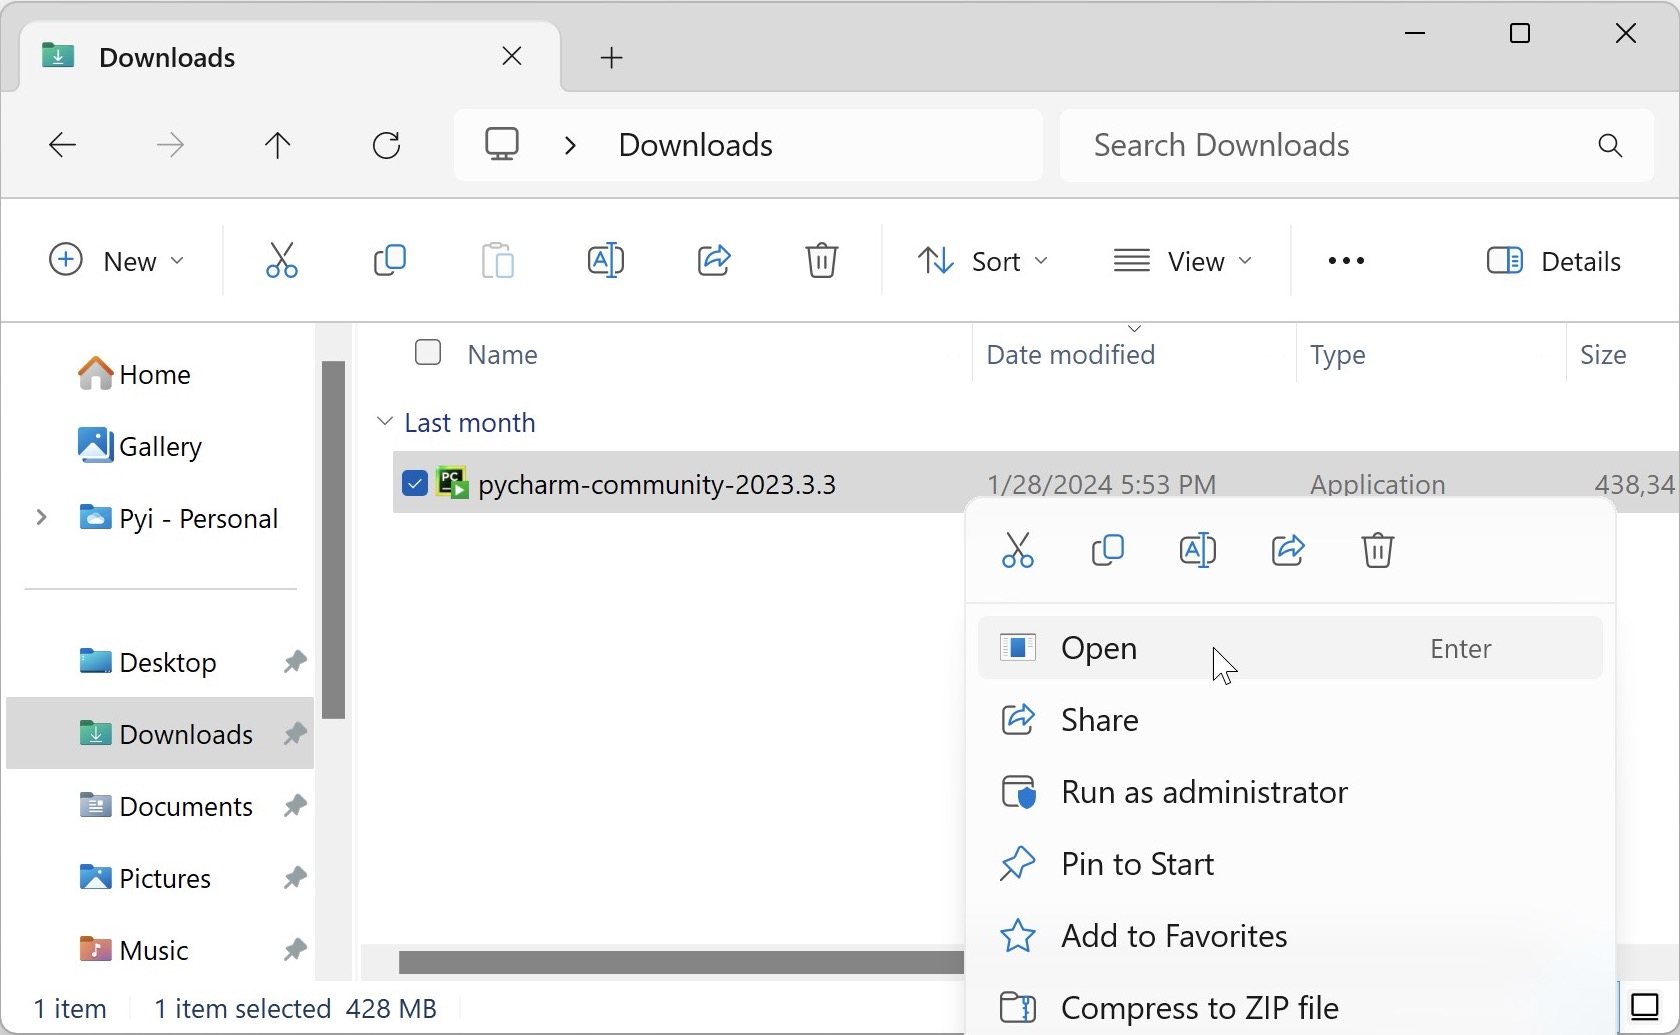
\includegraphics[width=.88\textwidth, trim={2.4mm 12cm 2mm 2mm},clip]{images/pycharm_install/2.jpg}};
    \drawshadow{image}
\end{tikzpicture}
\caption{} 
\label{fig:opnpychminstlr}
\end{figure}

\fEn{\mytcboxinl{PyCharm Community Edition}} ကို ဒေါင်းလုဒ်လုပ်ပါ။ (ဝဘ်စာမျက်နှာ အပေါ်ပိုင်းက ဝယ်သုံးရတဲ့ \fEn{\mytcboxinl{PyCharm Professional}} ကို ဒေါင်းလုဒ် မှားမလုပ်မိဖို့ သတိပြုပါ)။ အင်စတော်လာဖိုင်ကို ညာကလစ်နှိပ်ပြီး \fEnSnd{Open} လုပ်ပါ (ပုံ \fRefNo{\ref{fig:opnpychminstlr}} ကိုကြည့်ပါ)။ \fEnSnd{Yes/No} မေးတဲ့အခါ \fEnSnd{Yes} နှိပ်ပါ။ \mytcboxinl{\fEnSnd{Next >}} ကို နှိပ်၍ ရှေ့ကိုဆက်သွားပြီး နောက်ဆုံးမှာ \mytcboxinl{\fEnSnd{Install}} နှိပ်ပြီး ကွန်ဖန်းလုပ်ပါ။ အင်စတောလ်ပြီးသွားရင် \mytcboxinl{\fEnSnd{Finish}} နှိပ်ပါ။

ဝင်းဒိုး \fEnSnd{Taskbar Search} ကနေ \fEn{PyCharm} ကိုရှာပြီးဖွင့်ပါ (ပုံ \fRefNo{\ref{fig:schpychm}} ကို ကြည့်ပါ)။ သဘောတူကြောင်း ကွန်းဖန်းလုပ်ခိုင်းရင် ချက်ခ်ဘောက်စ် ချက်ခ်လုပ်ပြီး \mytcboxinl{\fEnSnd{Continue}} နှိပ်ပါ။  ဒေတာပို့ချင်လား ထပ်မေးပါလိမ့်မယ်။ \mytcboxinl{\fEnSnd{Don't Send}} နှိပ်ပါ။ \fEnSnd{Welcome} စခရင်ကိုပေါ်လာမယ်။ ပုံ (\fRefNo{\ref{fig:pychmwlcm}}) မှာ ကြည့်ပါ။




\todo{youtube facebook လင့်ထည့်ရန်}

\begin{mytcbox}
ဒီစာရေးနေချိန် လက်ရှိ \fEn{PyCharm} ဗားရှင်းက ၂၀၂၃ ပါ။ သိပ်မကြာခင် ၂၀၂၄ ထွက်ပါတော့မယ်။ အကယ်၍ လက်ရှိဗားရှင်းထက် နိမ့်တဲ့ဗားရှင်းတွေကို ဒေါင်းလုဒ် လုပ်ချင်ရင် အောက်ပါ လင့်ကို သွားပါ။ 
%
\begin{minted}[frame=lines, framerule=0pt]{text}
https://www.jetbrains.com/pycharm/download/other.html
\end{minted}
%
ဗားရှင်း ၂၀၂၄/၂၅ ထွက်ပြီးတဲ့ အချိန်မှာ ၂၀၂၃ ဗားရှင်းကို လိုချင်ရင် ဝဘ်စာမျက်နှာမှ ရှာပြီး ဒေါင်းလုဒ် လုပ်ပါ။ ၂၀၂၃ မှာလည်း ဗားရှင်းအခွဲတွေ ရှိပါသေးတယ်။ လက်ရှိအမြင့်ဆုံး ဗားရှင်းအခွဲ (ဥပမာ ၂၀၂၃.၃.၃) ကို သုံးလို့ရပါတယ်။ ၂၀၂၄/၂၅ သုံးမယ်ဆိုရင်လည်း ပြဿနာတော့ မရှိပါဘူး။ \fEn{Update} ဗားရှင်းဖြစ်တဲ့အတွက် ပုံတွေမှာ ပြထားတာနဲ့တော့ ကွာခြားချက်တချို့ ရှိကောင်းရှိနိုင်ပါတယ်။
\end{mytcbox}
%

\begin{figure}[tbh!]
\begin{tikzpicture}
    \node[anchor=south west,inner sep=0] (image) at (0,0)
        {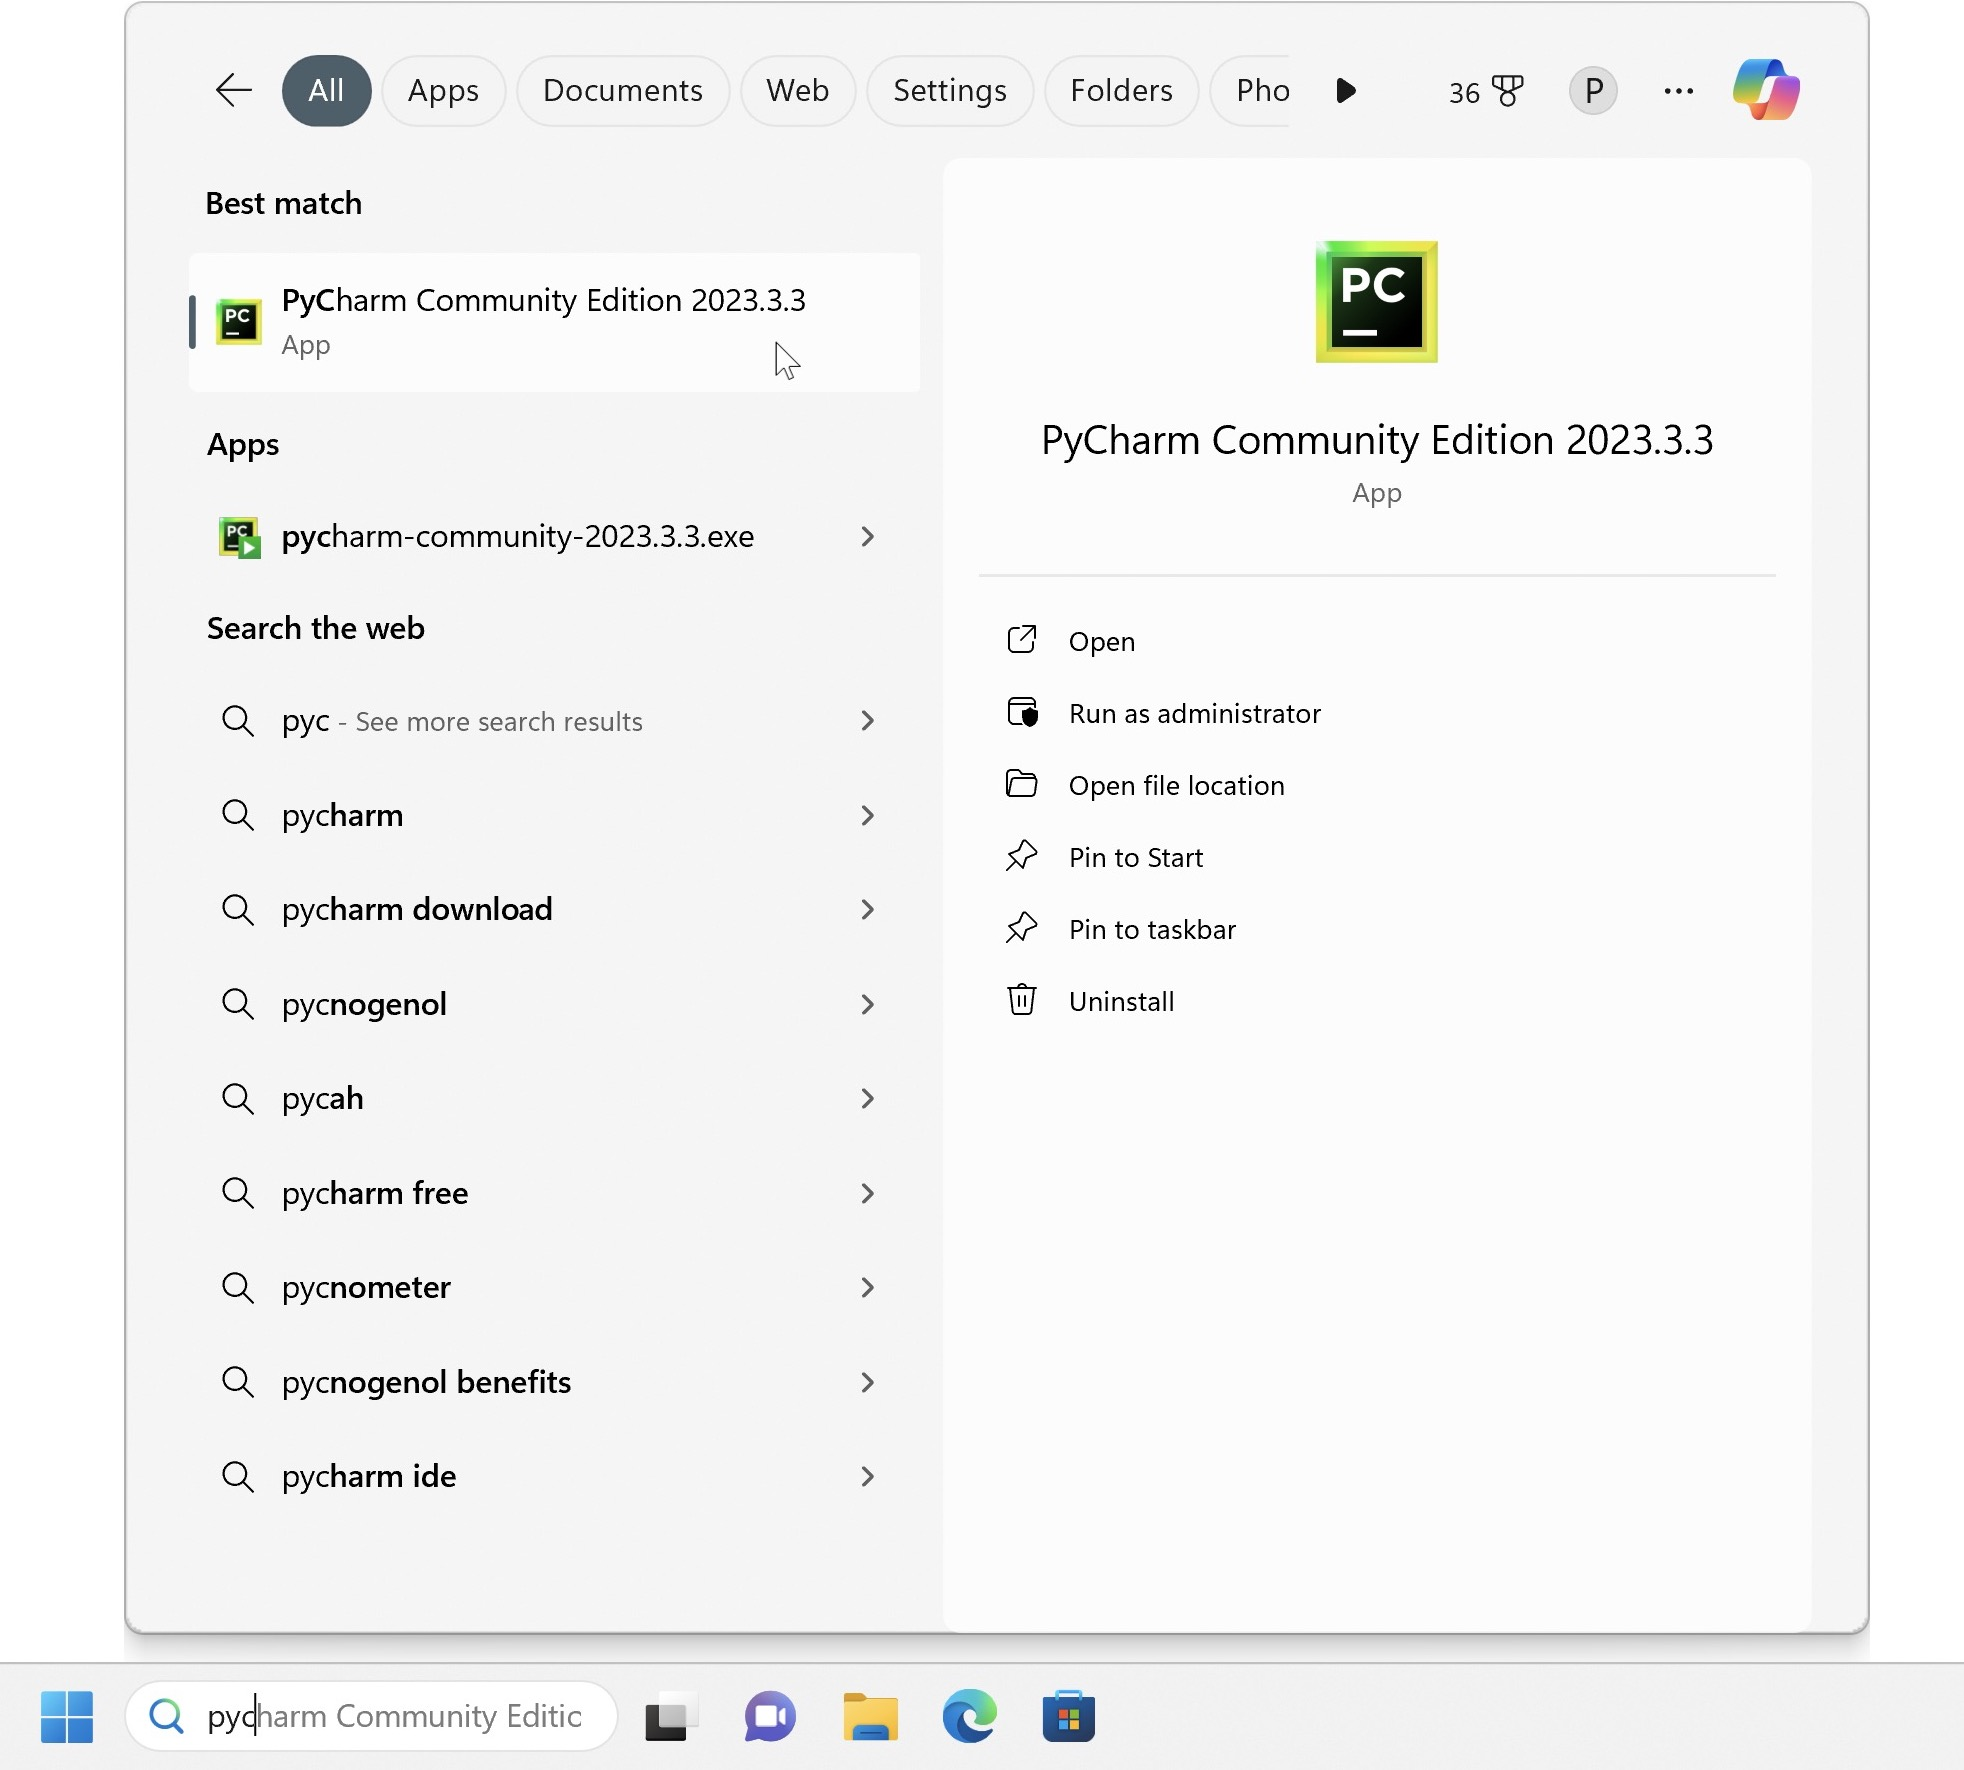
\includegraphics[width=.9\textwidth, trim={2.4mm 2mm 2mm 2mm},clip]{images/pycharm_install/3.jpg}};
    \drawshadow{image}
\end{tikzpicture}
\caption{} 
\label{fig:schpychm}
\end{figure}

\begin{figure}[H]
\begin{tikzpicture}
    \node[anchor=south west,inner sep=0] (image) at (0,0)
        {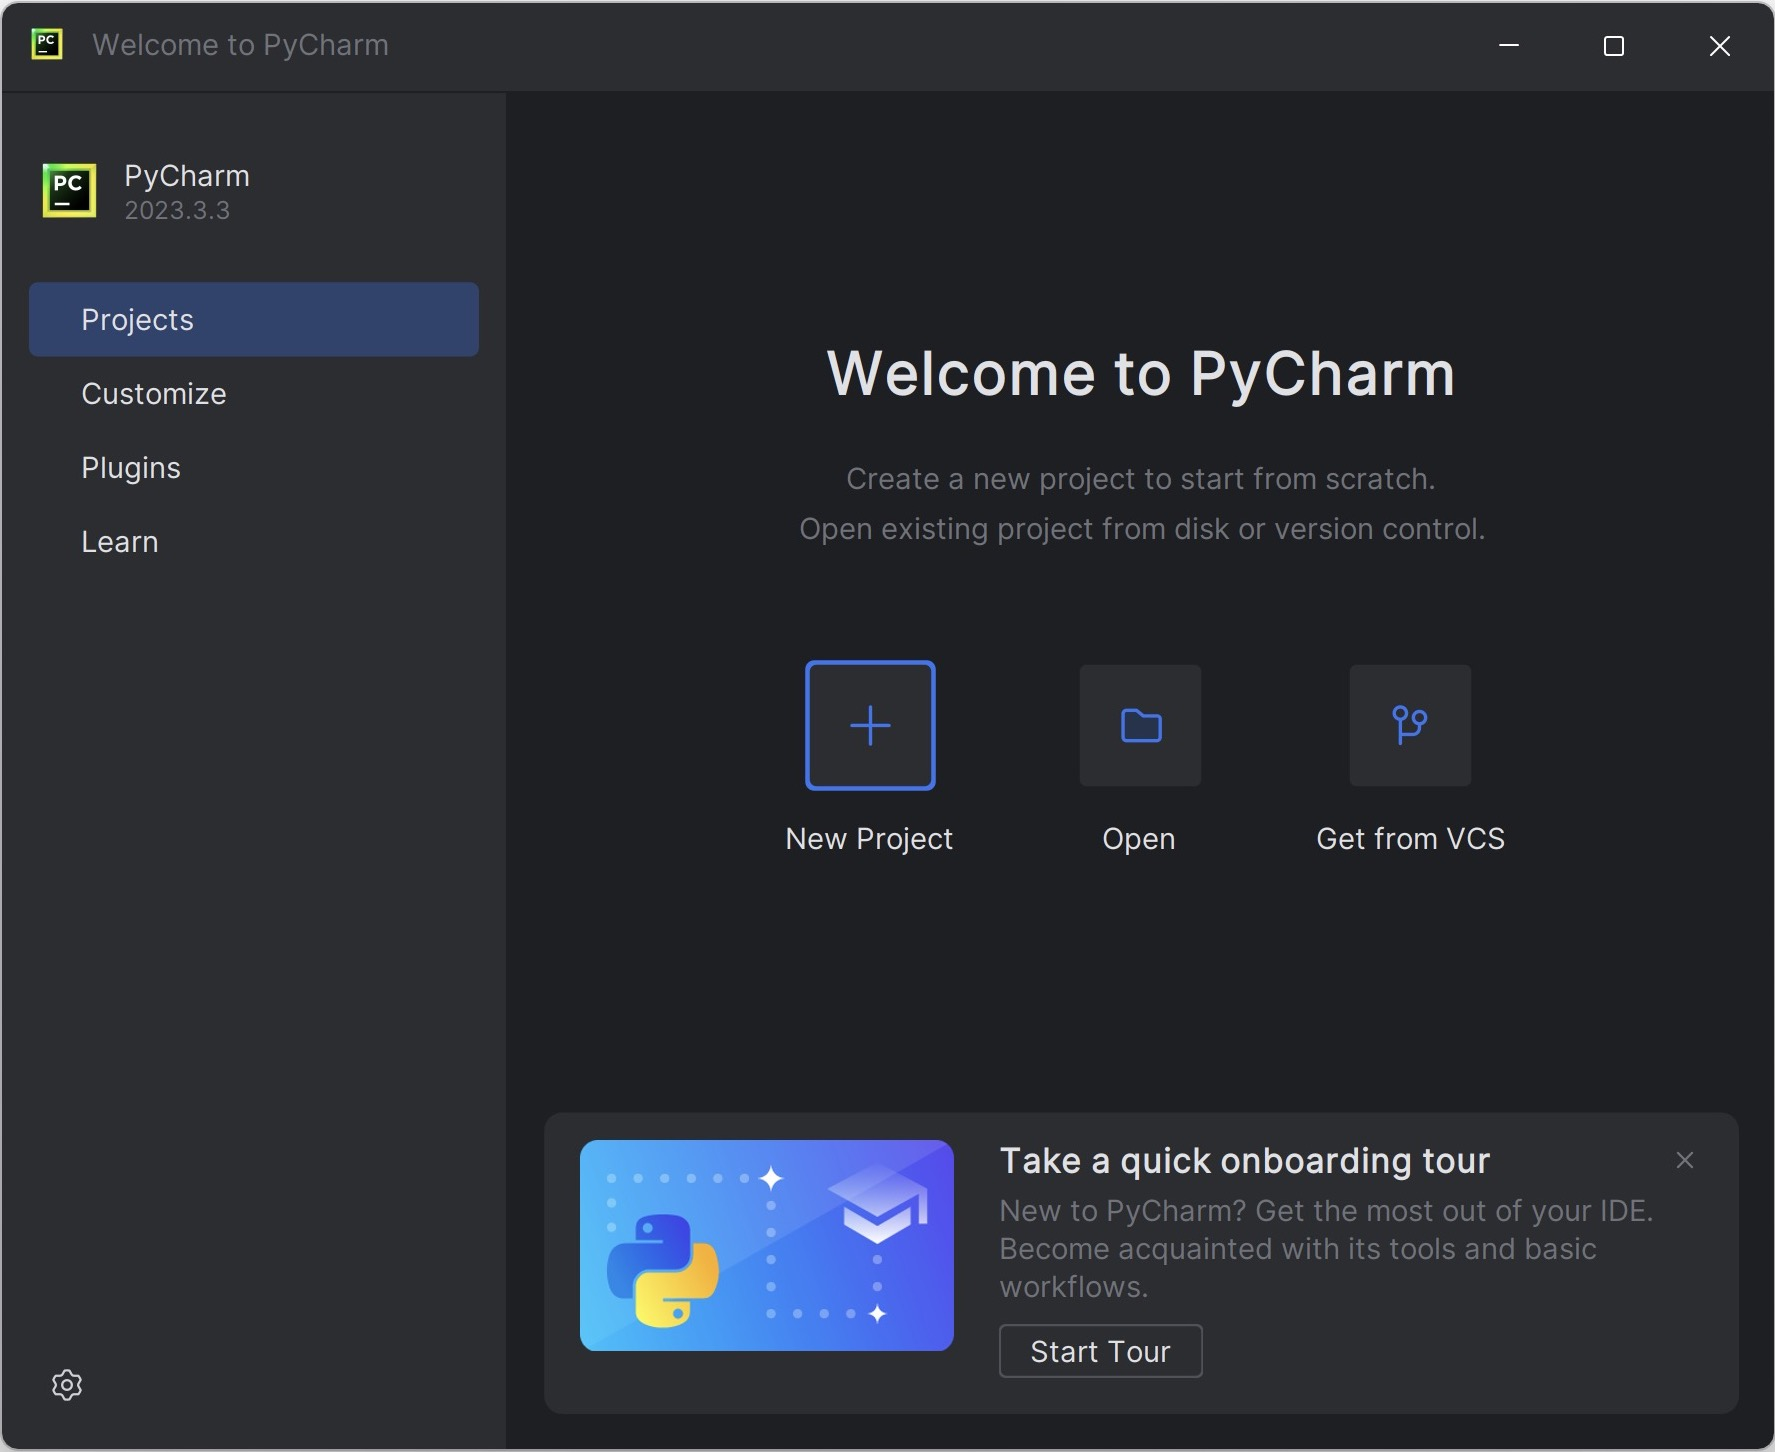
\includegraphics[width=.98\textwidth, trim={2.4mm 2mm 2mm 2mm},clip]{images/pycharm_install/4.jpg}};
    \drawshadow{image}
\end{tikzpicture}
\caption{} 
\label{fig:pychmwlcm}
\end{figure}

\subsection*{PyCharm IDE ဆိုတာဘာလဲ}
\fEn{PyCharm} ဟာ \fEn{Python} နဲ့ ဆော့ဖ်ဝဲ  ရေးဖို့အတွက် အထောက်အကူပြု \fEn{Integrated Development Environment(IDE)} ဆော့ဖ်ဝဲဖြစ်ပါတယ်။ စာစီစာရိုက်လုပ်တဲ့အခါ \fEn{Microsoft Word} ကို အသုံးပြုကြသလိုပဲ \fEn{Python} ကုဒ်ရေးဖို့ \fEn{PyCharm} ကိုသုံးတဲ့ သဘောပေါ့။ \fEn{PyCharm IDE} က \fEn{Python} ပရောဂျက်တွေ အတွက် အဓိကရည်ရွယ်တယ်။ အဆောက်အဦးတစ်ခု၊ တံတားတစ်ခု ဆောက်လုပ်တာကို ပရောဂျက်လို့ ပြောလေ့ရှိသလို ပရိုဂရမ်/ဆော့ဖ်ဝဲတစ်ခု တည်ဆောက်တာကိုလည်း ပရောဂျက်လို့ပဲ သုံးနှုန်းပါတယ်။ တစ်ဦးတစ်ယောက်တည်း ရေးတဲ့ ပရိုဂရမ်အသေးလေးတွေ အတွက် \fEn{PyCharm} ကို အသုံးပြုနိုင်သလို ပရိုဂရမ်မာတွေ အဖွဲ့လိုက်နဲ့ တည်ဆောက်ရတဲ့ ပရောဂျက်ကြီးတွေ အတွက်လည်း သုံးပါတယ်။ ဒီစာအုပ်မှာတော့ \fEn{PyCharm} ရဲ့ အဆင့်မြင့်ဖီချာတွေကို အသုံးပြုမှာ မဟုတ်ပါဘူး။ ပရိုဂရမ်းမင်း စလေ့လာသူတွေကို လွယ်ကူအဆင်ပြေစေတဲ့ အခြေခံ ဖီချာတွေလောက်ပဲ အသုံးပြုမှာပါ။ 

\clearpage

\subsection*{PyCharm ပရောဂျက်ဆောက်ခြင်း}
အင်စတောလ်လုပ်ပြီးရင် \fEn{PyCharm IDE} ကိုဖွင့်ပြီး \fEnSnd{Welcome} စခရင်မှ သိုမဟုတ် \fEnSnd{File} မီနူးမှ \fEnSnd{New Project} နှိပ်ပြီး ပရောဂျက် အသစ်ယူပါ (ပြီးခဲတဲ့ ပုံ \fRefNo{\ref{fig:pychmwlcm}} ကို ပြန်ကြည့်ပါ)။ နံမည်ကို \fEnSnd{MeetKarel} ပေးပါ။ ပုံ (\fRefNo{\ref{fig:new_proj}}) မှာ တွေ့ရတဲ့အတိုင်း \fEnSnd{\mytcboxinl{Pure Python}, \mytcboxinl{Proj venv}} နဲ့ \fEn{Python} ဗားရှင်း \fEnSnd{3.12.xx} ကို ရွေးပါ။ \fEnSnd{xx} က အခြားဂဏန်း ဖြစ်နေနိုင်တယ်။ အဓိက ဗားရှင်း \fEnSnd{3.12} သာ ဖြစ်ပါစေ။ \fEnSnd{Create} ခလုတ်နှိပ်ပါ။ ပရောဂျက်အတွက် \fEn{Python} ကို အင်စတောလ် လုပ်ပါလိမ့်မယ်။

မိမိလေ့လာနေတဲ့ အခန်းတစ်ခန်းချင်းစီအတွက် ပရောဂျက်တစ်ခု ဆောက်နိုင်ပါတယ်။ အခန်း (၂) အတွက် \fEnSnd{Chapter02} ၊ အခန်း (၃) အတွက် \fEnSnd{Chapter03} စသည်ဖြင့်။  သက်ဆိုင်ရာအခန်းအလိုက် ကုဒ်ဖိုင်တွေကို ပရောဂျက်တစ်ခုစီမှာ ထားတဲ့အတွက် ဖိုင်တွေများပြီး ရှုပ်ထွေဖောင်းပွနေတဲ့ ပြဿနာ မရှိတော့ဘူး။ ကုဒ်ဖိုင်တွေကို ပရောဂျက်တစ်ခုထဲမှာပဲ ဖိုဒါအလိုက်ခွဲထားလို့ရပေမဲ့ စလေ့လာသူအနေနဲ့ ပရောဂျက်တစ်ခုချင်း ခွဲထားတာလောက် မလွယ်ကူဘူး။

ပရောဂျက် အသစ်ယူတဲ့အခါ တည်နေရာ \mytcboxinl{\fEnSnd{Location:}} ကို သူ့နဂိုအတိုင်း ထားနိုင်သလို မိမိထားချင်တဲ့နေရာကို ညာဘက်စွန်း ဖိုဒါအိုင်ကွန်လေးနှိပ်ပြီး ပြောင်းလို့ရတယ်။

\begin{figure}[tb!]
\begin{tikzpicture}
    \node[anchor=south west,inner sep=0] (image) at (0,0)
        {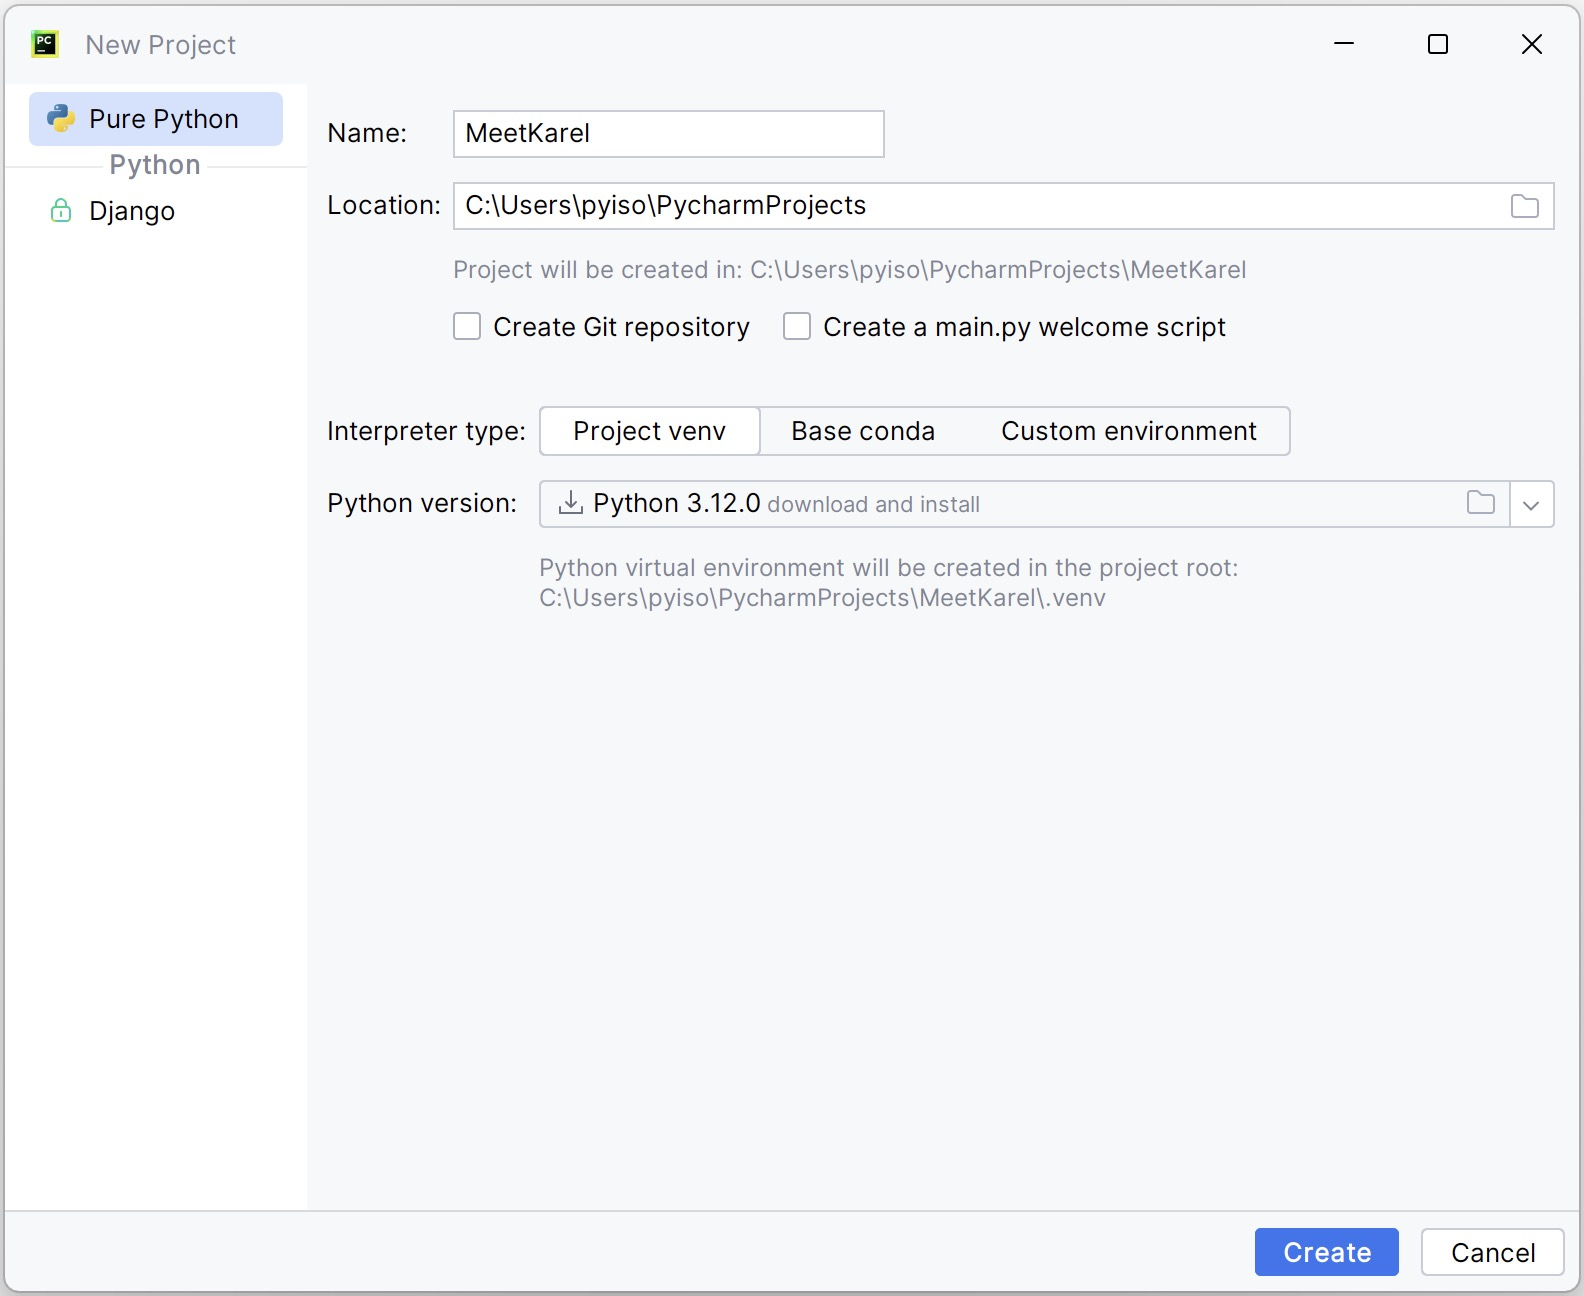
\includegraphics[width=.98\textwidth, trim={2.3mm 2mm 2mm 2.3mm},clip]{images/pycharm_install/new_proj.jpg}};
    \drawshadow{image}
    \draw [draw=red,very thick,rounded corners] (0.15,9.82) rectangle (2.3,9.31);
    \draw [draw=red,very thick,rounded corners] (4.3,7.27) rectangle (6.21,6.76);
    \draw [draw=red,very thick,rounded corners] (4.3,6.68) rectangle (8,6.17);

\end{tikzpicture}
\caption{ပရောဂျက် အသစ်ယူခြင်း} 
\label{fig:new_proj}
\end{figure}

\begin{figure}[tb!]
\begin{tikzpicture}
    \node[anchor=south west,inner sep=0] (image) at (0,0)
        {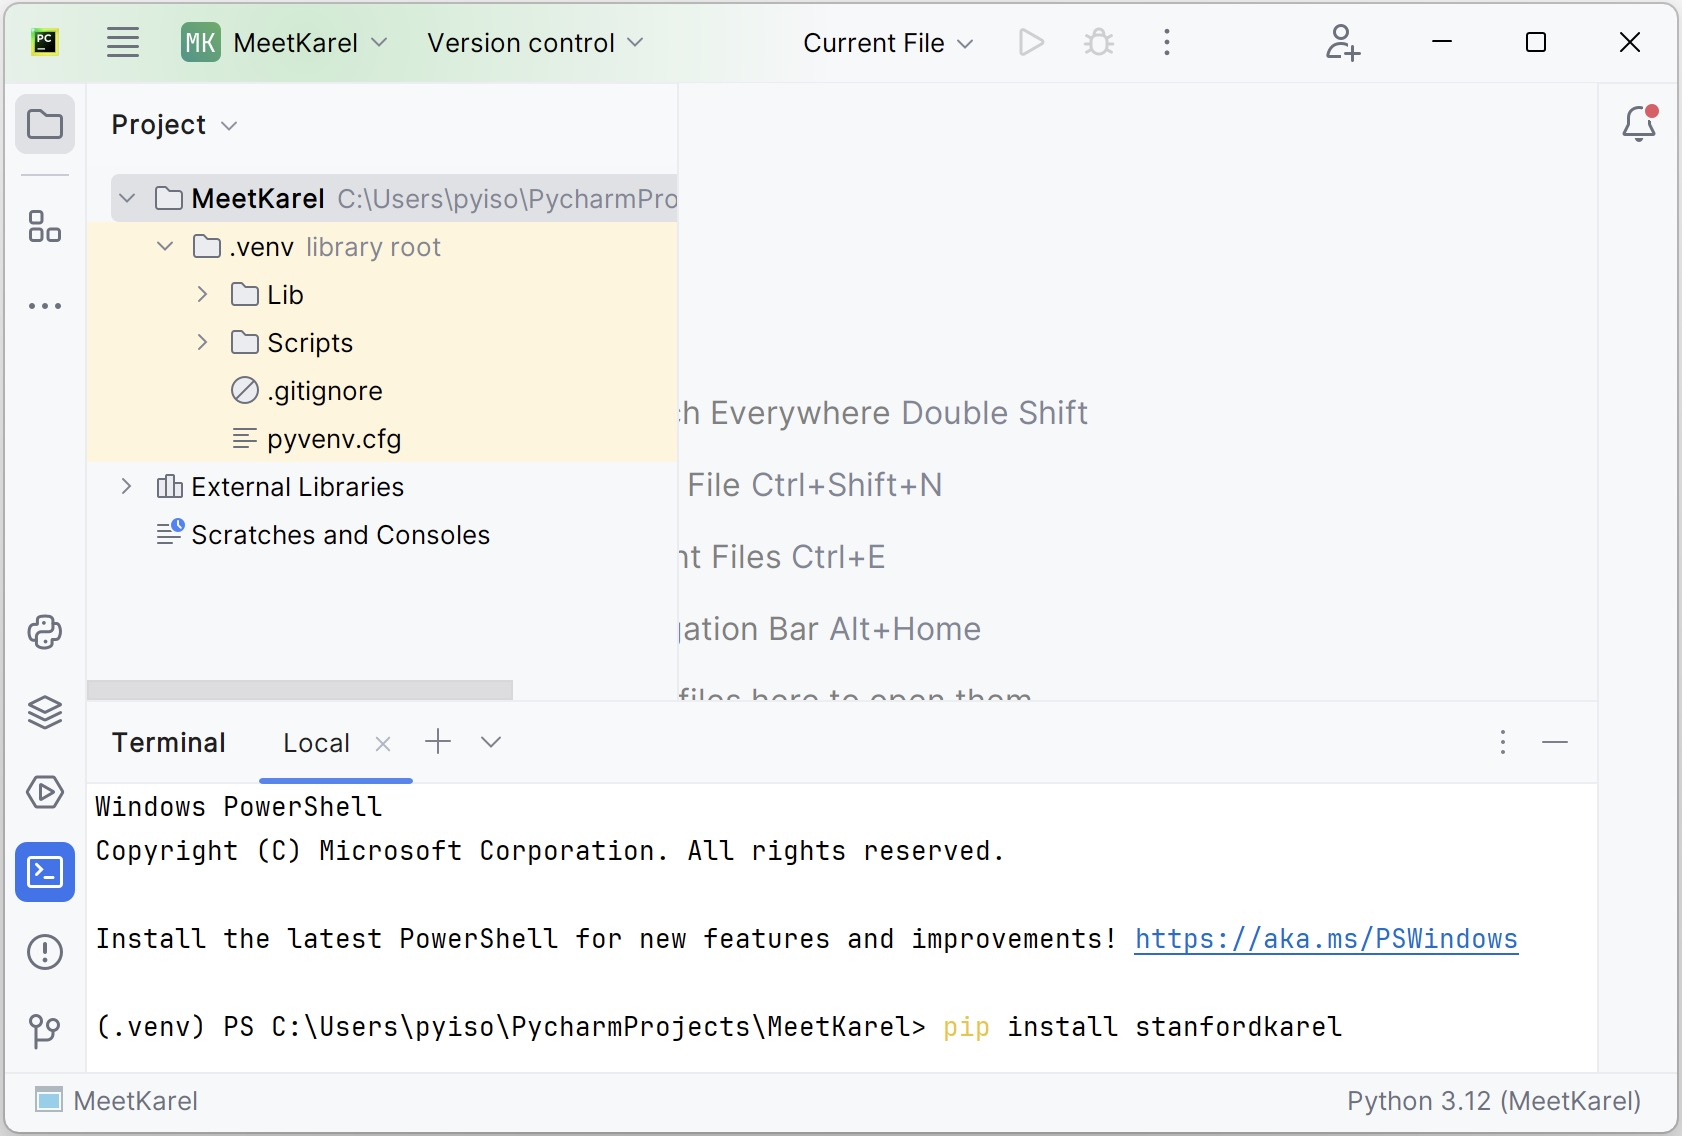
\includegraphics[width=.98\textwidth, trim={2.4mm 2mm 2mm 2.4mm},clip]{images/pycharm_install/install_karel.jpg}};
    \drawshadow{image}
    \draw [draw=red,very thick,rounded corners] (0.02,2.26) rectangle (0.57,1.71);
    \draw [draw=red,very thick,rounded corners] (7.13,1.1) rectangle (10.4,0.55);
\end{tikzpicture}
\caption{Karel လိုက်ဘရီ အင်စတောလ်လုပ်ခြင်း} 
\label{fig:install_karel}
\end{figure}

\subsection*{stanfordkarel လိုက်ဘရီ အင်စတောလ်လုပ်ခြင်း}
ပုံ (\fRefNo{\ref{fig:install_karel}}) မှာ အနီရောင် ဝိုင်းပြထားတဲ့ အိုင်ကွန်ကို နှိပ်ပြီး \fEnSnd{Terminal} ကိုဖွင့်ပါ။ \fEnSnd{Terminal} မှာ အောက်ပါ ကွန်မန်းဖြင့် 
%
\begin{minted}[frame=lines, framerule=0pt]{text}
pip install stanfordkarel
\end{minted}
%
ကားရဲလ်လိုက်ဘရီကို အင်စတောလ်လုပ်ပါ။ ပုံ (\fRefNo{\ref{fig:install_karel}}) မှာ  အနီရောင် ဝိုင်းပြထားပါတယ်။ ခဏကြာတဲ့အခါ အခုလို \fOpn{မက်ဆေ့ချ်}တွေ ကျလာပါလိမ့်မယ်။ 

%
\begin{minted}[frame=lines, framerule=0pt,escapeinside=ßß]{text}
Collecting stanfordkarel
  Downloading stanfordkarel-0.2.7-py3-none-any.whl (51 kB)
     ━━━━━━━━━━━━━━━━━━━━━━━━━━━━━━━━━━━━━━━━ 51.9/51.9 kB 443.1 kB/s 
    eta 0:00:00
Installing collected packages: stanfordkarel
ß\colorbox{yellow}{Successfully installed stanfordkarel-0.2.7}ß

[notice] A new release of pip is available: 23.2.1 -> 24.0
[notice] To update, run: python.exe -m pip install --upgrade pip
(.venv) PS C:\Users\pyiso\PycharmProjects\MeetKarel>
\end{minted}
%
ဟိုက်လိုက်ပြထားတဲ့ \fOpn{မက်ဆေ့ချ်} တွေ့ရရင် အင်စတောလ်လုပ်တာ အောင်မြင်လို့ပါ။

\begin{mytcbox}
မှတ်ချက်။\qquad ။ ပရောဂျက် အသစ်ဆောက်တိုင်း လိုအပ်တဲ့ လိုက်ဘရီကို တစ်ခါထပ်ပြီး အင်စတောလ် လုပ်ရပါမယ်။ ကားရဲလ်အခန်း ပရောဂျက်တစ်ခုစီအတွက် \fEnSnd{stanfordkarel} လိုက်ဘရီကို အထက်ဖော်ပြပါအတိုင်း အင်စတောလ် လုပ်ဖို့လိုတယ်။
\end{mytcbox}

\clearpage
\subsection*{နမူနာ ကားရဲလ် ကမ္ဘာနှင့် ပရိုဂရမ်ကုဒ် ဖိုင်များထည့်ခြင်း}
\fEnSnd{meet\_karel.zip} ဖိုင်ကို \todo{ဒေါင်းလုဒ်လင့်ထည့်ရန်} ဒီလင့် \fCode{http://tinyurl.com/3mmm9c7j} ကနေ ဒေါင်းလုဒ်လုပ်ပါ။ ၎င်း \fEnSnd{zip} ဖိုင်ကို \fEn{extract} လုပ်ပါ။ \fEnSnd{meet\_karel} နံမည်နဲ့ ဖိုဒါတစ်ခု ရလာပါမယ်။ ၎င်းဖိုဒါထဲမှ အောက်ပါ \fEnSnd{worlds} ဖိုဒါနှင့် \fEnSnd{.py} ဖိုင်အားလုံးကို ကော်ပီလုပ်ပါ။ 
%
\begin{itemize}
    \item \fEnSnd{worlds} 
    \begin{itemize}
        \item \fEnSnd{meet\_karel.w}
        \item \fEnSnd{move\_beeper\_to\_other\_side.w}
    \end{itemize}
    \item \fEnSnd{meet\_karel.py}
    \item \fEnSnd{move\_beeper\_to\_other\_side.py}
    \item \fEnSnd{world\_editor.py}
\end{itemize}
%

\fEnSnd{MeetKarel} ပရောဂျက်ထဲတွင် ကူးထည့်ပါ။ ပင်မ ပရောဂျက် \fEnSnd{MeetKarel} (ပုံ \fRefNo{\ref{fig:edit_meet_karel}} မှာ မြှားပြထား) ပေါ်မှာ ညာကလစ်နှိပ်ပြီး \fEnSnd{Paste} လုပ်ရမှာပါ။ ကော်ပီကူးထည့်လိုက်တဲ့ ဖိုင်တွေက ပုံမှာ တွေ့ရတဲ့အတိုင်း  \fEnSnd{MeetKarel} ဖိုဒါအောက်မှာ ရှိသင့်ပါတယ်။

\begin{mytcbox}
အခန်းအလိုက် နမူနာ ကုဒ်ဖိုင်တွေ ထည့်ပေးထားတဲ့ \fEnSnd{.zip} ဖိုင်တွေကိုလည်း အထက်ပါအတိုင်း အလားတူ လုပ်ရပါမယ်။ ပရောဂျက်အသစ်ဆောက်၊ \fEnSnd{.zip} ဖိုင်ကို ဖြည်၊ ရလာတဲ့ ဖိုဒါထဲက ဖိုင်တွေကို ပင်မ ပရောဂျက် ဖိုဒါထဲ ကော်ပီကူးထည့် ရုံပါပဲ။
\end{mytcbox}

\fEnSnd{meet\_karel.py} ဖိုင်ကို ကလစ်နှစ်ချက်နှိပ် ဖွင့်ပါ။ ပုံ (\fRefNo{\ref{fig:edit_meet_karel}}) မှာ အနီဝိုင်းထားတဲ့  ကုဒ်အယ်ဒီတာ \fEn{(code editor)} ပွင့်လာပါမယ်။ အဲဒီ မူရင်းဖိုင်မှာ အောက်ပါအတိုင်း ဆက်လက် ပြင်ဆင်ဖြည့်စွက်ပါ။
%
\setlength{\fboxsep}{0pt}
\label{lst:mtkrl}
\begin{minted}[frame=\mintframe, framerule=\mintrule,framesep= \mintsep, xleftmargin=\xlftmargin
                , bgcolor=mintbgcolor,rulecolor=mintrulecolor
                , python3=true]{python}
from stanfordkarel import *


def main():
    """Karel code goes here!"""
    move()
    move()
    move()
    pick_beeper()
    turn_left()
    move()
    move()

    turn_left()
    turn_left()
    turn_left()

    move()
    put_beeper()


if __name__ == "__main__":
    run_karel_program("meet_karel")
\end{minted}
%

%http://tinyurl.com/3mmm9c7j
%https://bit.ly/42MhViS

% google drive root folder
%http://tinyurl.com/mkamnasm
%https://bit.ly/3T3tgrA

\begin{mytcbox}
\fEn{run} ထားတဲ့ ပရိုဂရမ်တစ်ခုကို တစ်ခါထပ် \fEn{run} ရင် \mytcboxinl{\fEnSnd{Cancel}} (သို့) \mytcboxinl{\fEnSnd{Stop and Rerun}} လုပ်မှာလားမေးတယ်။ \mytcboxinl{\fEnSnd{Stop and Rerun}} လုပ်ရပါတယ်။
\end{mytcbox}

\fEnSnd{meet\_karel.py} ဖိုင်ကို ညာကလစ်နှိမ်ပြီး \fEnSnd{\mytcboxinl{Run 'meet\_karel'}} လုပ်ပါ (အယ်ဒီတာ ဧရိယာမှာ ညာကလစ်နှိမ်ပြီး \fEnSnd{\mytcboxinl{Run 'meet\_karel'}} လုပ်လို့လည်း ရပါတယ်) ။ ပုံ (\fRefNo{\ref{fig:mtkrlpgm}}) က ကားရဲလ် ပရိုဂရမ် တက်လာရင် \fEnSnd{\mytcboxinl{Run Program}} ခလုတ်ကိုနှိပ်ပါ။ ဘိပါကို ကားရဲလ်က ရွှေ့ပေးပါလိမ့်မယ်။

\begin{figure}[b!]
\begin{tikzpicture}
    \node[anchor=south west,inner sep=0] (image) at (0,0)
        {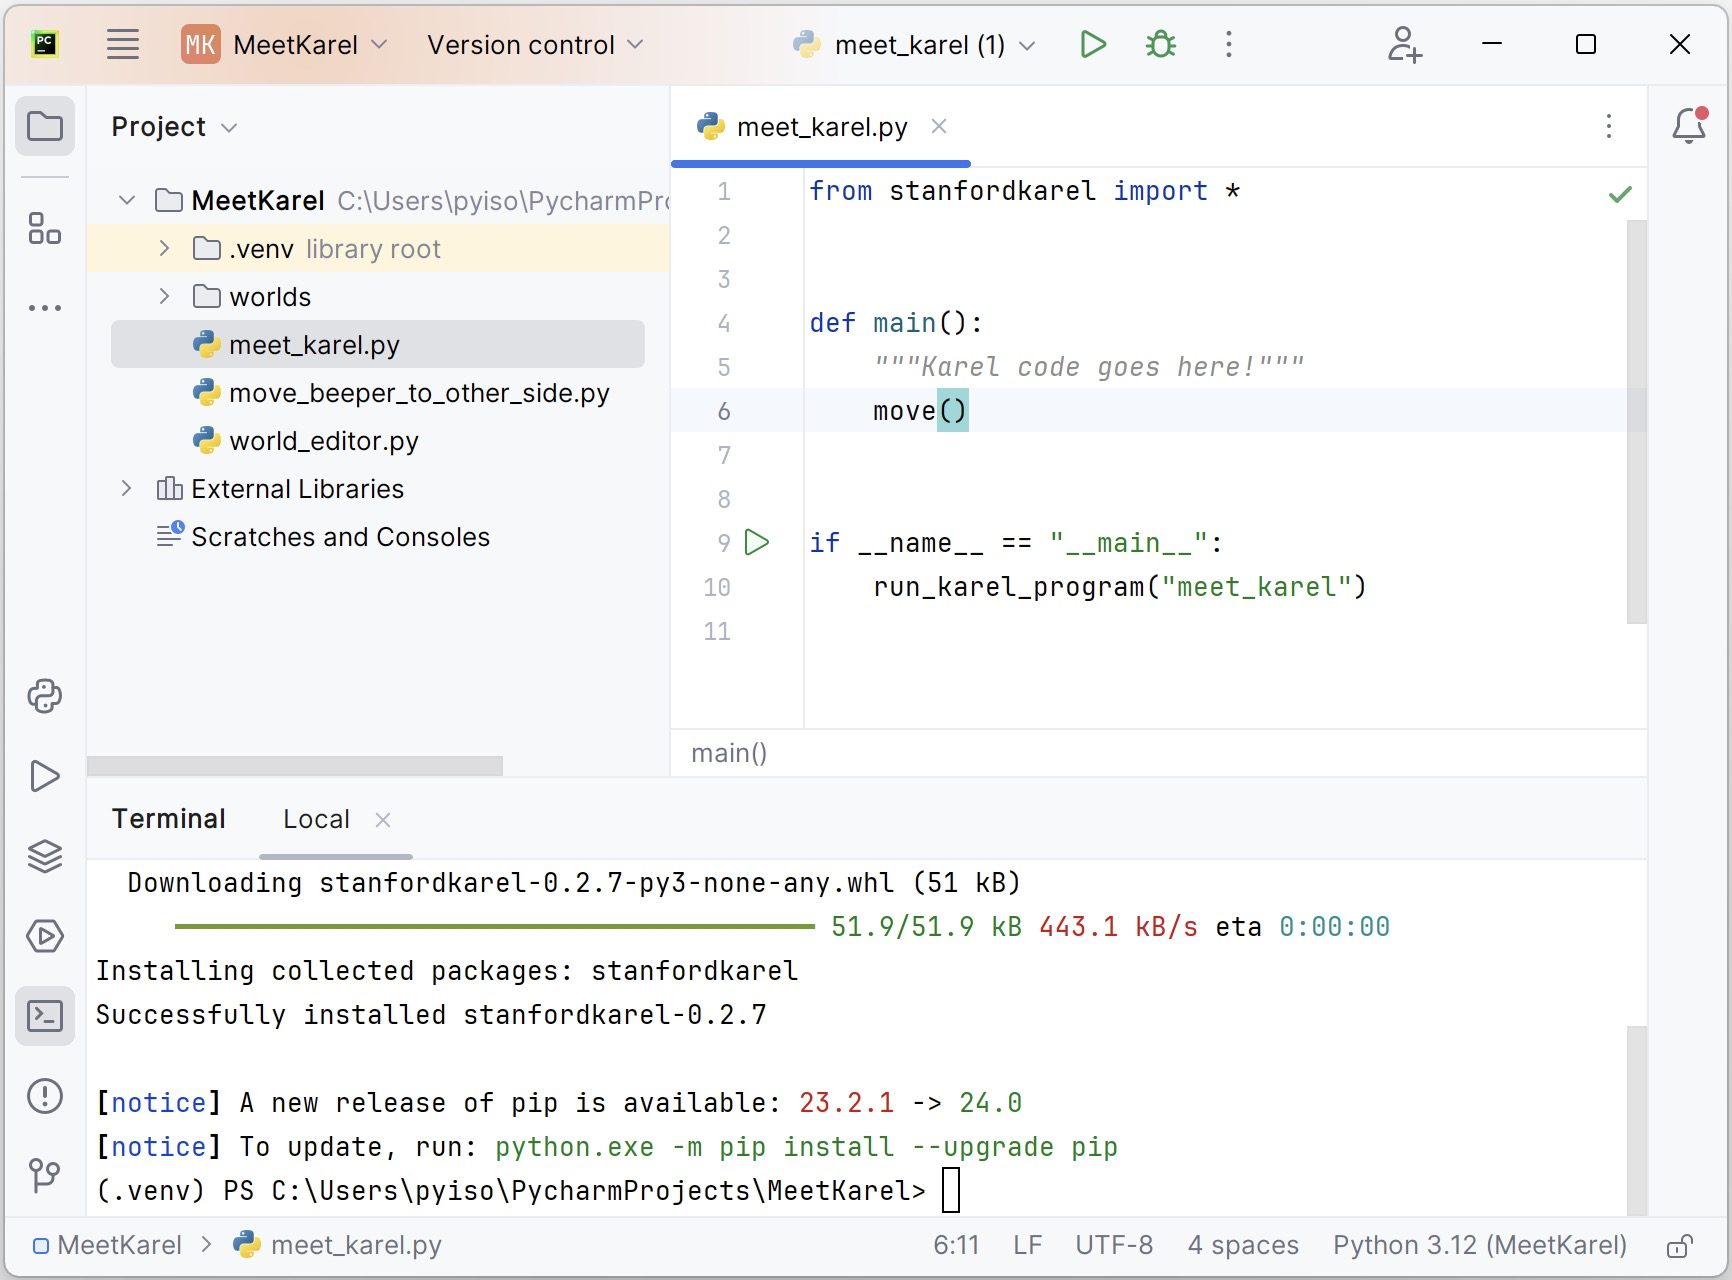
\includegraphics[width=.98\textwidth, trim={2.4mm 2mm 2mm 2.4mm},clip]{images/pycharm_install/edit_meet_karel.jpg}};
    \drawshadow{image}
    
    \draw[-{Latex[length=3mm]}, very thick, red](3, 9)-- (2 ,8.15);
    \draw [draw=red, thick,rounded corners] (5, 8.87) rectangle (12.25 ,3.75);
\end{tikzpicture}
\caption{} 
\label{fig:edit_meet_karel}
\end{figure}


\begin{figure}[b!]
\begin{tikzpicture}
    \node[anchor=south west,inner sep=0] (image) at (0,0)
        {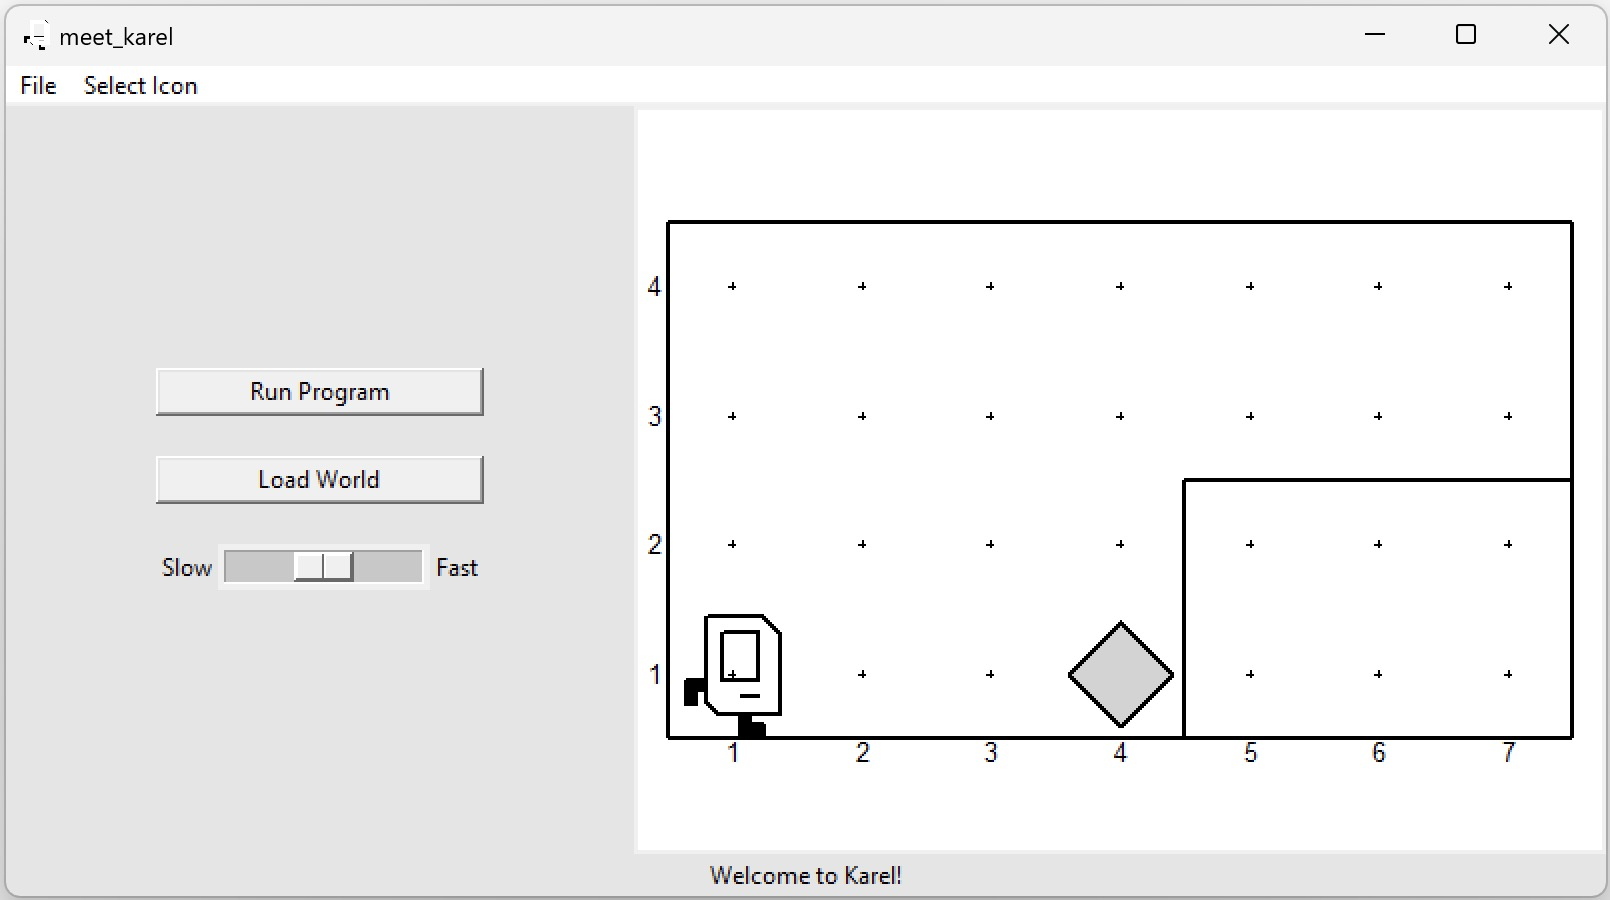
\includegraphics[width=.82\textwidth, trim={2.4mm 2cm 2mm 2mm},clip]{images/pycharm_install/meet_karel_program.jpg}};
    \drawshadow{image}
\end{tikzpicture}
\caption{} 
\label{fig:mtkrlpgm}
\end{figure}



\clearpage
\subsection*{ဆင်းတက်စ်အမှားများ}
\begin{figure}[b!]
\begin{tikzpicture}
    \node[anchor=south west,inner sep=0] (image) at (0,0)
        {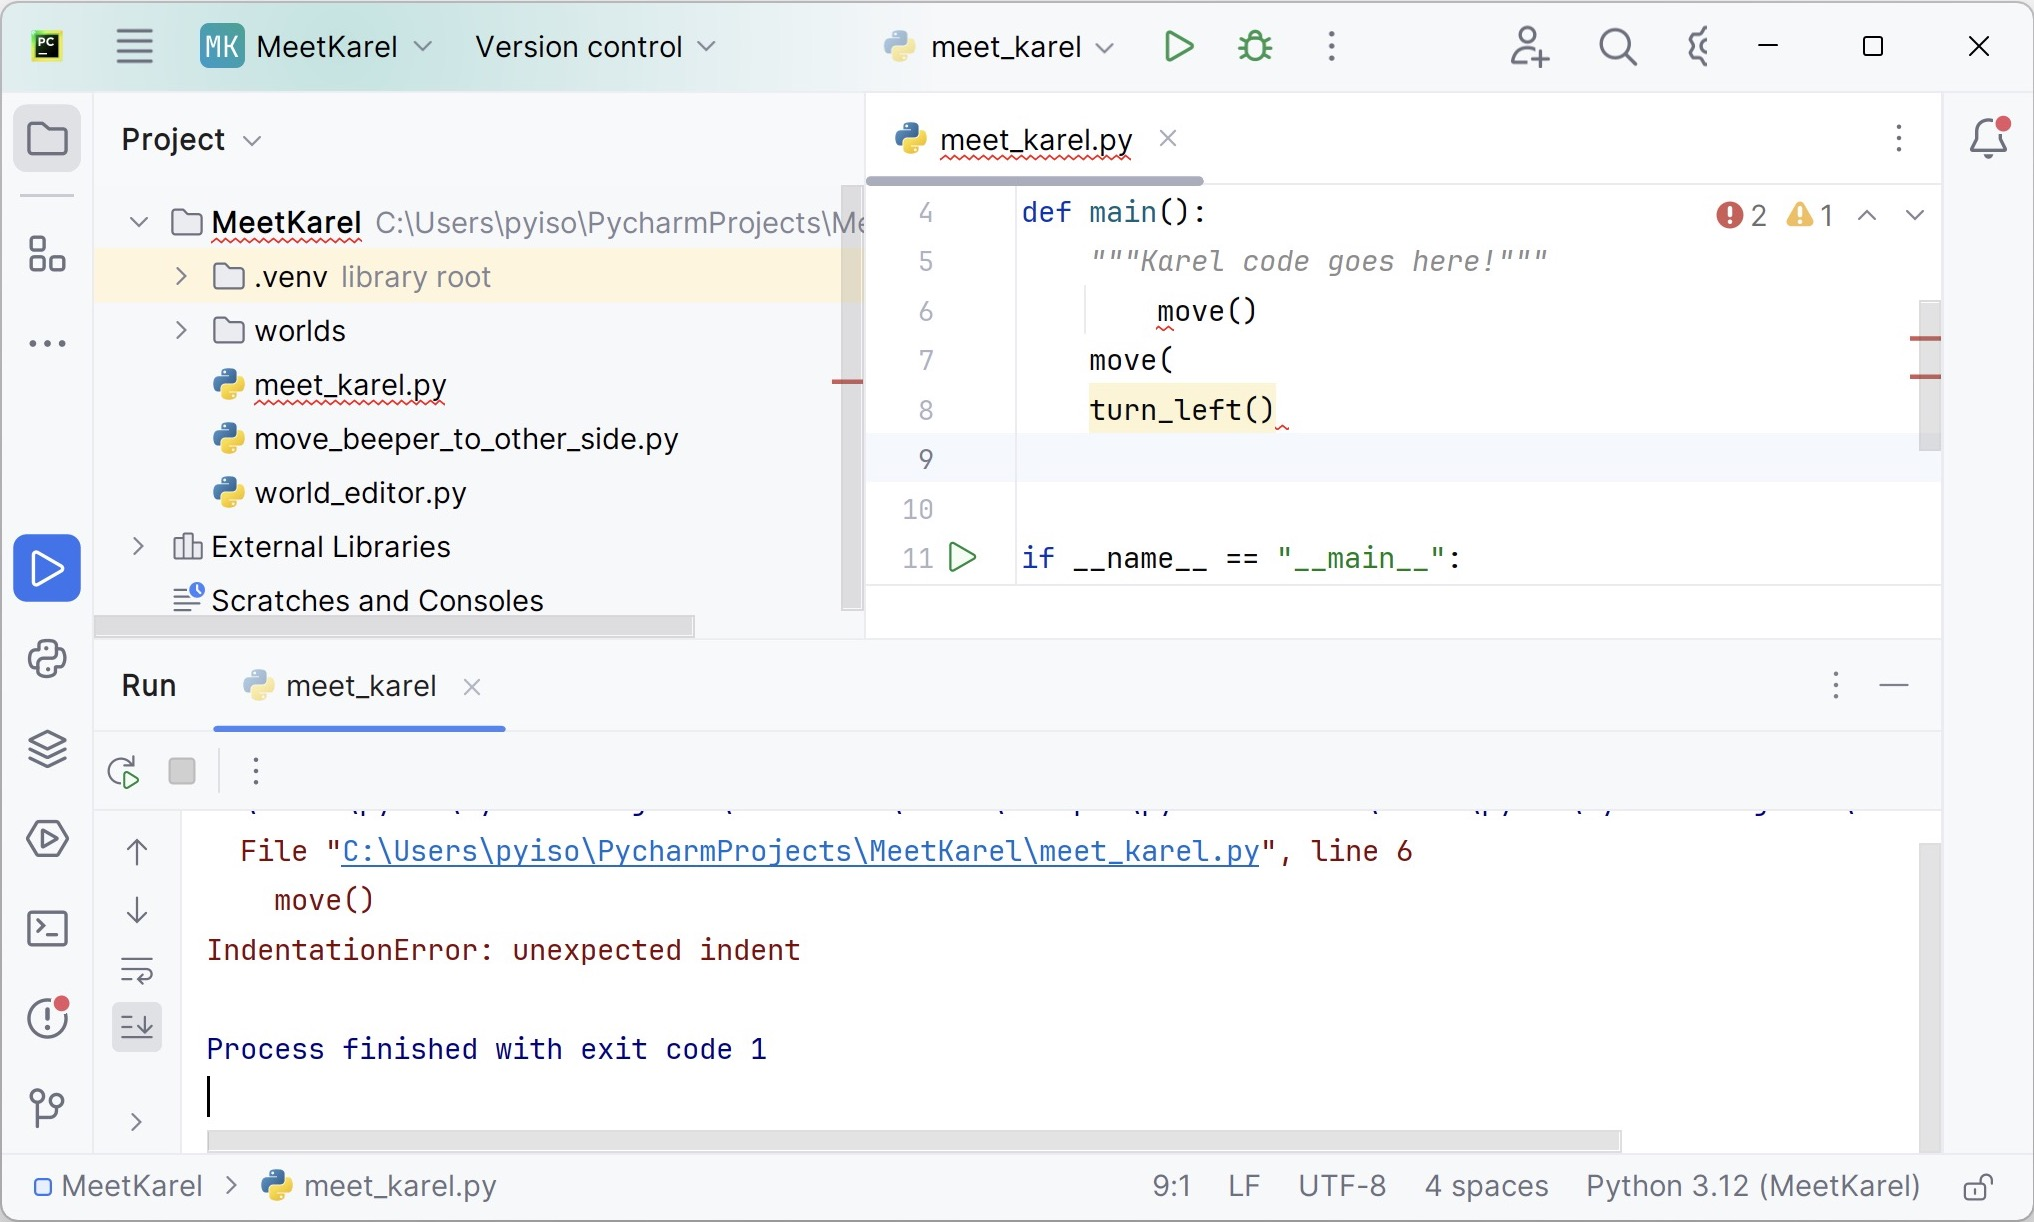
\includegraphics[width=.98\textwidth, trim={2.4mm 2mm 2mm 2mm},clip]{images/pycharm_install/sntxerr.jpg}};
    \drawshadow{image}
\end{tikzpicture}
\caption{} 
\label{fig:sntxerr}
\end{figure}
အကယ်၍ ပရိုဂရမ် \fEn{run} လို့မရရင် ကုဒ်ရေးတာမှားနေလို့ ဖြစ်နိုင်တယ်။ မိမိရေးထားတာကို စာမျက်နှာ (\fRefNo{\pageref{lst:mtkrl}}) က ပရိုဂရမ်ကုဒ်နဲ့  နှိုင်းယှဉ် စစ်ဆေးကြည့်ပါ။ \fEn{PyCharm} အယ်ဒီတာမှာ အနီလှိုင့်တွန့်လေးတွေ (ပုံ \fRefNo{\ref{fig:sntxerr}}) ပြတဲ့နေရင် အဲဒီနေရာတွေမှာ ဆင်းတက်စ်မှားနေလို့ (သို့) လိုက်ဘရီမထည့်ရသေးလို့ပဲ။

ဝိုက်ကွင်းကျန်နေတာက အဖြစ်များတဲ့ အမှားပါ။ ကျန်ခဲ့လို မရပါဘူး။ အင်ဒန့်တေးရှင်း \fEn{(indentation)} လုပ်ရမဲ့နေရာမှာ မလုပ်ထားရင်လည်း ပြဿနာဖြစ်တယ်။ \fCode{move}\fEn{,} \fCode{turn\_left} တွေကို ဘေးမျဉ်းညာဘက်ခွာပြီး အင်ဒန့်လုပ်ပေးရမယ်။ အဲဒါတွေ ဂရုမစိုက်မိရင် ဆင်းတက်စ်အမှားဖြစ်ပြီး ပရိုဂရမ် \fEn{run} လို့ မရနိုင်ဘူး။

\fEnSnd{Terminal} မှာ ထုတ်ပေးတဲ့ \fOpn{မက်ဆေ့ချ်}တွေကို ကြည့်ပြီးတော့လည်း ဘာပြဿနာဖြစ်နေလဲ မှန်းဆလို့ရနိုင်တယ်။ ဘာကြောင့်ဖြစ်နိုင်လဲ ဆက်စပ်စဉ်းစားလို့ ရတယ်။ ဥပမာ ဖြစ်တဲ့ပြဿနာအလိုက် အခုလိုတွေ့ရပါမယ်။ 
%
\begin{minted}[frame=lines, framerule=0pt,escapeinside=ßß]{text}
File "c:\Users\pyiso\VS Code\meet_karel\meet_karel.py", ß\mytcboxinl[yellow]{line 6}ß
    move(
          ^
    ß\mytcboxinl[yellow]{SyntaxError: '(' was never closed}ß
\end{minted}
%
%
\begin{minted}[frame=lines, framerule=0pt,escapeinside=ßß]{text}
File "c:\Users\pyiso\VS Code\meet_karel\meet_karel.py", ß\mytcboxinl[yellow]{line 7}ß
    move()
    ß\mytcboxinl[yellow]{IndentationError: unexpected indent}ß 
\end{minted}
%
%
\begin{minted}[frame=lines, framerule=0pt, escapeinside=ßß]{text}
Traceback (most recent call last):
  File "c:\Users\pyiso\VS Code\meet_karel\meet_karel.py", ß\mytcboxinl[yellow]{line 1}ß, 
        in <module>
    from stanfordkarel import *
    ß\mytcboxinl[yellow]{ModuleNotFoundError: No module named 'stanfordkarel'}ß
\end{minted}
%
\clearpage

\subsection*{Python ဖိုင် အသစ်ယူခြင်း}
\fEnSnd{MeetKarel} ပင်မ ပရောဂျက်ဖိုဒါပေါ်မှာ ညာကလစ်နှိပ်ပြီး \fEn{Python} ဖိုင် အသစ်ယူနိုင်ပါတယ်။ \fEn{Python} ဖိုင်တွေက \fEnSnd{.py} အိပ်စ်တန်းရှင်းနဲ့ပါ။ ကားရဲလ်ပရိုဂရမ်တစ်ခုကို \fEn{Python} ဖိုင်တစ်ခု ထားပါမယ်။ ပင်မ ပရောဂျက်ဖိုဒါ အောက်မှာပဲ တိုက်ရိုက်ရှိရပါမယ်။ 

နောက်ပိုင်း အဆင့်မြင့်လာရင် ပရိုဂရမ်တစ်ခုအတွက် ပရောဂျက်တစ်ခု ထားနိုင်တယ်။ ကုဒ်ဖိုင်တွေအပြင် ပရိုဂရမ်အတွက် လိုအပ်တဲ့ ရုပ်ပုံတွေ၊ အခြားဖိုင်တွေ (\fEn{config} ဖိုင်၊ \fEn{setting} ဖိုင် စသည်ဖြင့်) လည်း ပါနိုင်တယ်။ ပင်မပရောဂျက် အောက်မှာပဲ  ဖိုင်တွေက တိုက်ရိုက်ရှိဖို့လည်း မလိုတော့ဘူး။  ဆက်{\allowbreak}စပ်ရာ ဖိုင်တွေကို အမျိုးအစားအလိုက်၊  ဖန်ရှင်အလိုက် ဖိုဒါတွေခွဲပြီး  စနစ်ကျ စီစဉ်ဖွဲ့စည်း ထားရမှာပါ။ ပရောဂျက်တစ်ခုမှာ ဖိုင်တွေကို စနစ်တကျ စုဖွဲ့ထားဖို့ အရေးကြီးပါတယ်။

\begin{figure}[tbh!]
\begin{tikzpicture}
    \node[anchor=south west,inner sep=0] (image) at (0,0)
        {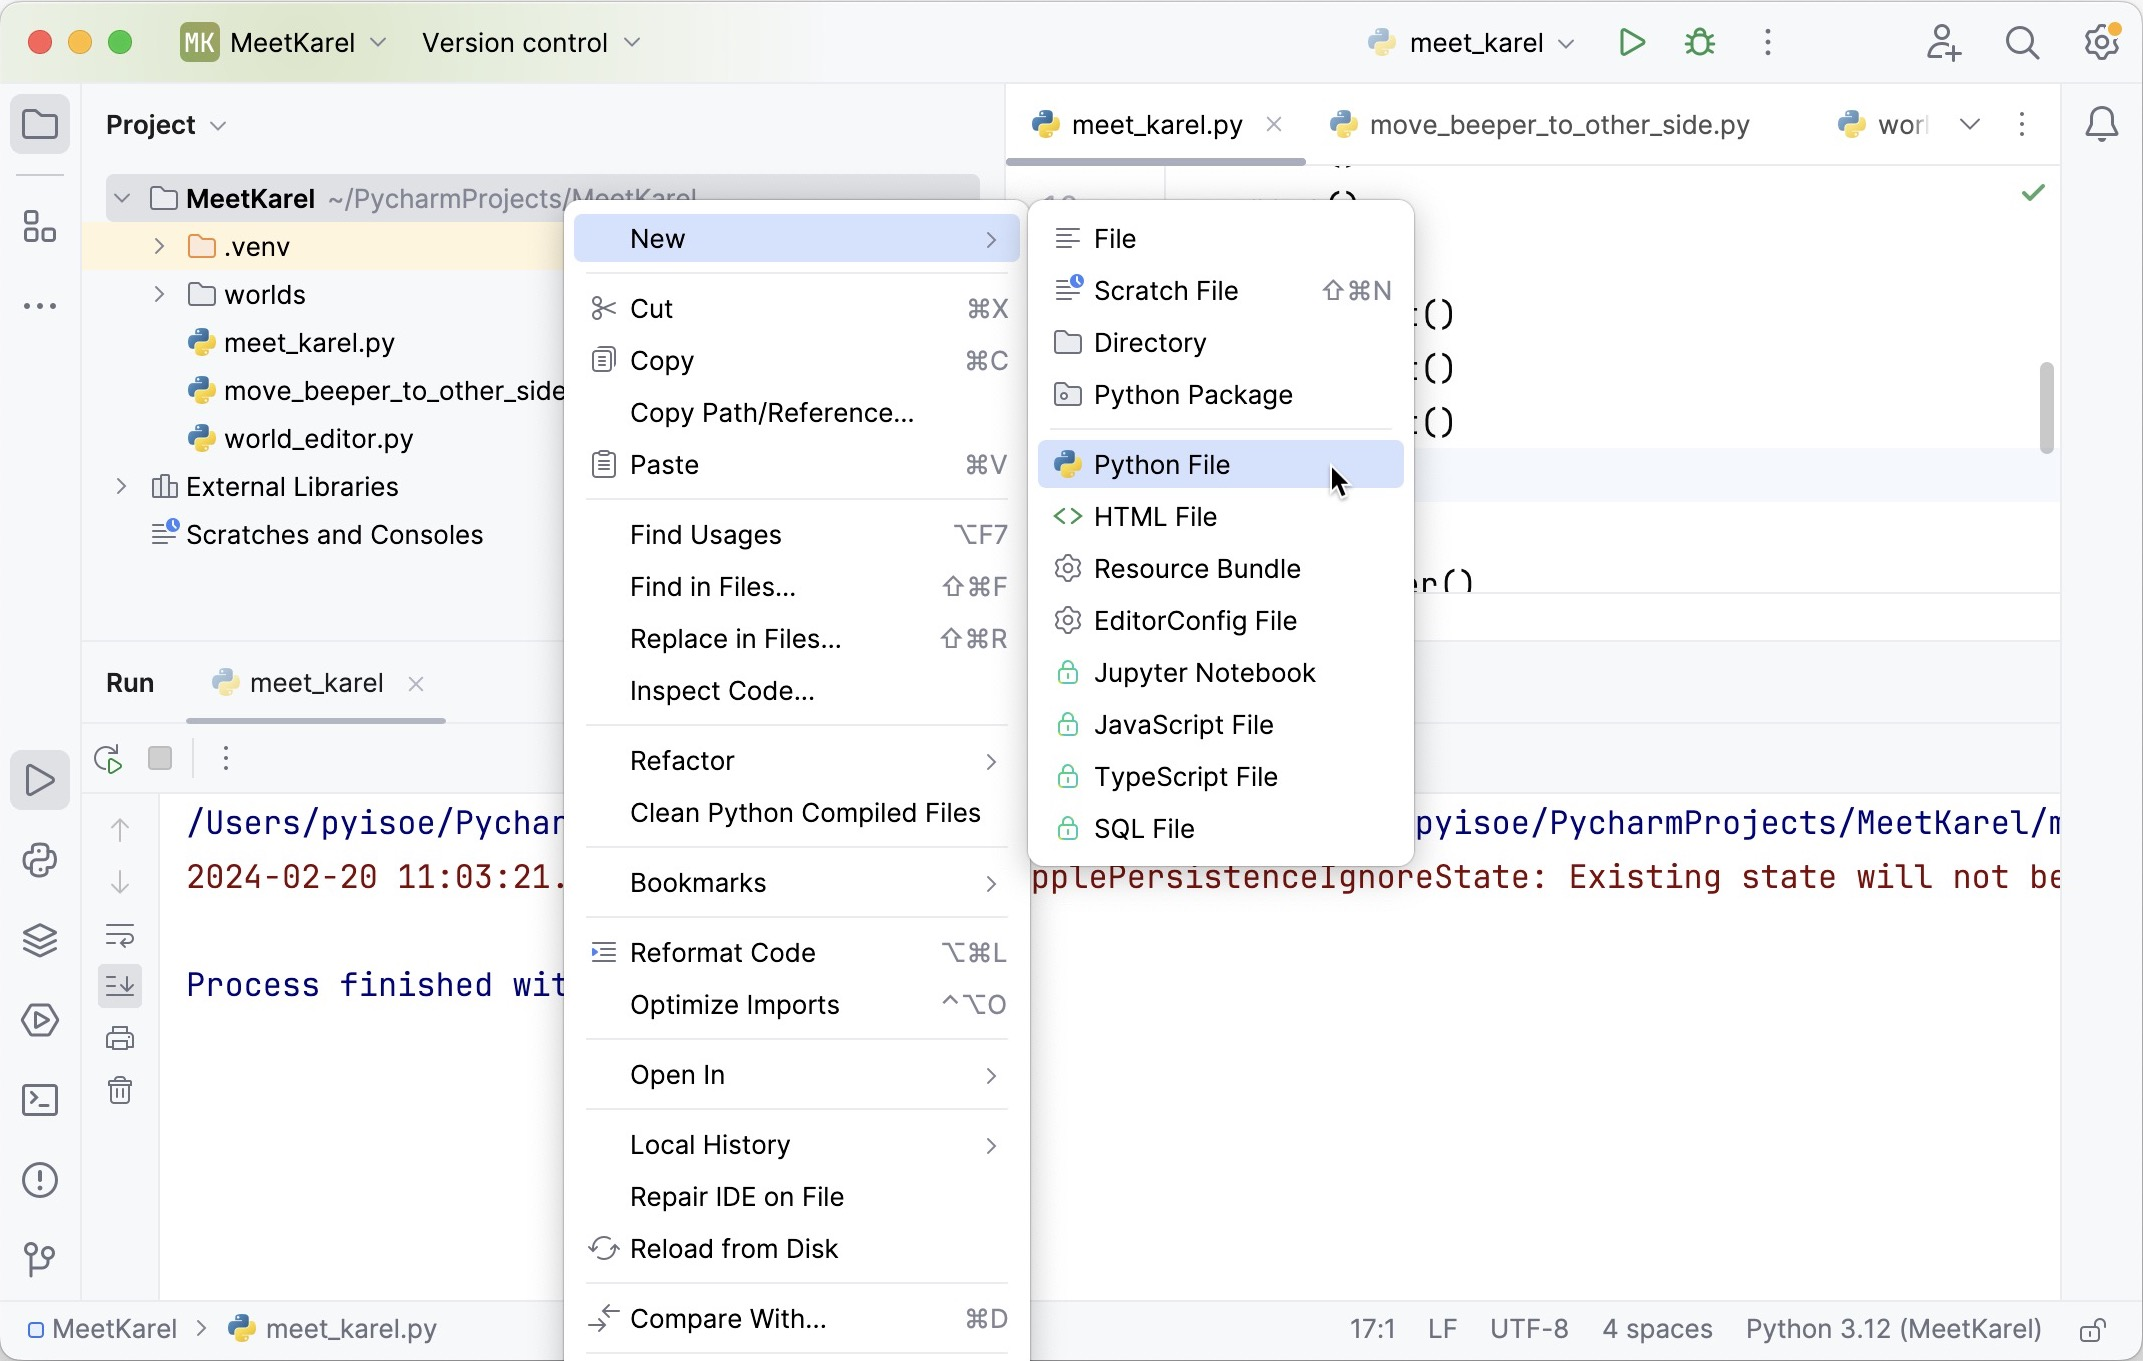
\includegraphics[width=.98\textwidth, trim={2.4mm 2mm 2mm 2mm},clip]{images/pycharm_install/newfile.jpg}};
    \drawshadow{image}
\end{tikzpicture}
\caption{} 
\label{fig:newfile}
\end{figure}

\clearpage



\section*{Visual Studio Code နှင့် Python အင်စတောလ်လုပ်ခြင်း}
\fEn{Visual Studio Code(VS Code)} ဟာ ပရိုဂရမ်မာအများစု ကြိုက်နှစ်သက်တဲ့ မော်ဒန် ကုဒ်အယ်ဒီတာ တစ်ခုပါ။ \fEn{Python, JavaScript, C++} စတဲ့ \fEn{programming language} အမျိုးမျိုးအတွက် အသုံးပြုနိုင်ပါတယ်။

\fEn{PyCharm} မှာတော့ ပရောဂျက်အသစ်ဆောက်ရင် \fEn{Python} ပါ တစ်ခါတည်း ဒေါင်းလုဒ်လုပ်ပြီး အင်စတောလ် လုပ်လို့ရတယ်။  \fEn{VS Code} နဲ့ \fEn{Python} ရေးမယ်ဆိုရင် \fEn{Python Programming Language} ကို သီးခြား ဒေါင်းလုဒ်လုပ်ပြီး အင်စတောလ် လုပ်ရပါမယ်။ 
\subsection*{Python အင်စတောလ်လုပ်ခြင်း}\label{subsec:pyinstl}
ဒီလင့် \fCode{https://www.python.org/} ကိုဖွင့်ပါ။ \fEnSnd{Download} မီနူးမှ \fEnSnd{Windows} နှိပ်ပါ (ပုံ \fRefNo{\ref{fig:pyhome}} ကိုကြည့်ပါ)။ \fEn{Apple} ကွန်ပျူတာအတွက် ဆိုရင် \fEnSnd{macOS} ရွေးရပါမယ်။ လူများစုသုံးတဲ့ မိုက်ခရိုဆော့ဖ် ဝင်းဒိုးအတွက် အင်စတောလ်လုပ်နည်းကို အဓိကပြပေးမှာပါ။ ပုံ \fRefNo{\ref{fig:pyvers}} မှာလို တွေ့ရပါလိမ့်မယ်။ အင်စတော်လာ ဗားရှင်း \fEn{3.12} ထဲက လက်ရှိအမြင့်ဆုံး ကိုရွေးပါ။ ဒီစာရေးချိန်မှာ \fEn{3.12.2} ဟာ အမြင့်ဆုံးဗားရှင်းပါ။ \mytcboxinl{\fEnSnd{Windows Installer (64-bit)}} ကိုနှိပ်ပြီး ဒေါင်းလုဒ်လုပ်ပါ။

\todo{linux အတွက် ဖော်ပြရန်}
\begin{figure}[tbh!]
\begin{tikzpicture}
    \node[anchor=south west,inner sep=0] (image) at (0,0)
        {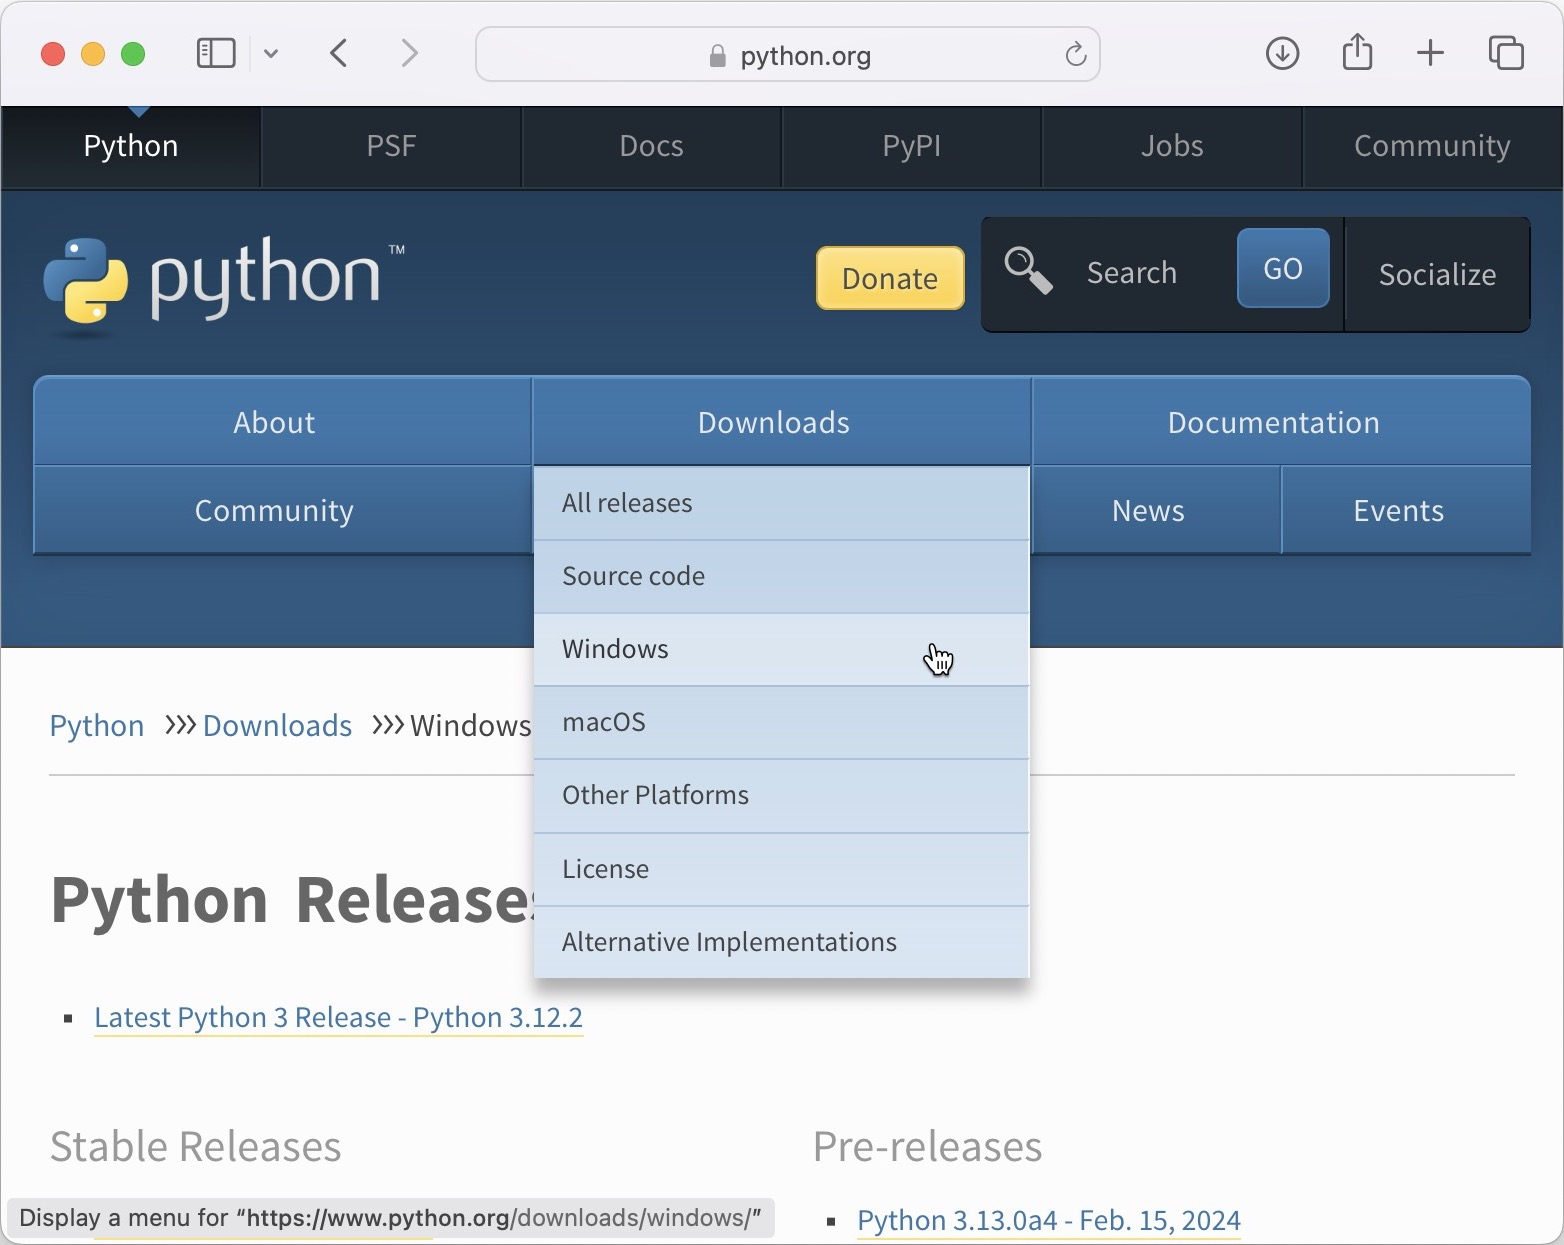
\includegraphics[width=.98\textwidth, trim={2.4mm 2mm 2mm 2mm},clip]{images/vscode_install/1.jpg}};
    \drawshadow{image}
\end{tikzpicture}
\caption{} 
\label{fig:pyhome}
\end{figure}

\begin{figure}[tbh!]
\begin{tikzpicture}
    \node[anchor=south west,inner sep=0] (image) at (0,0)
        {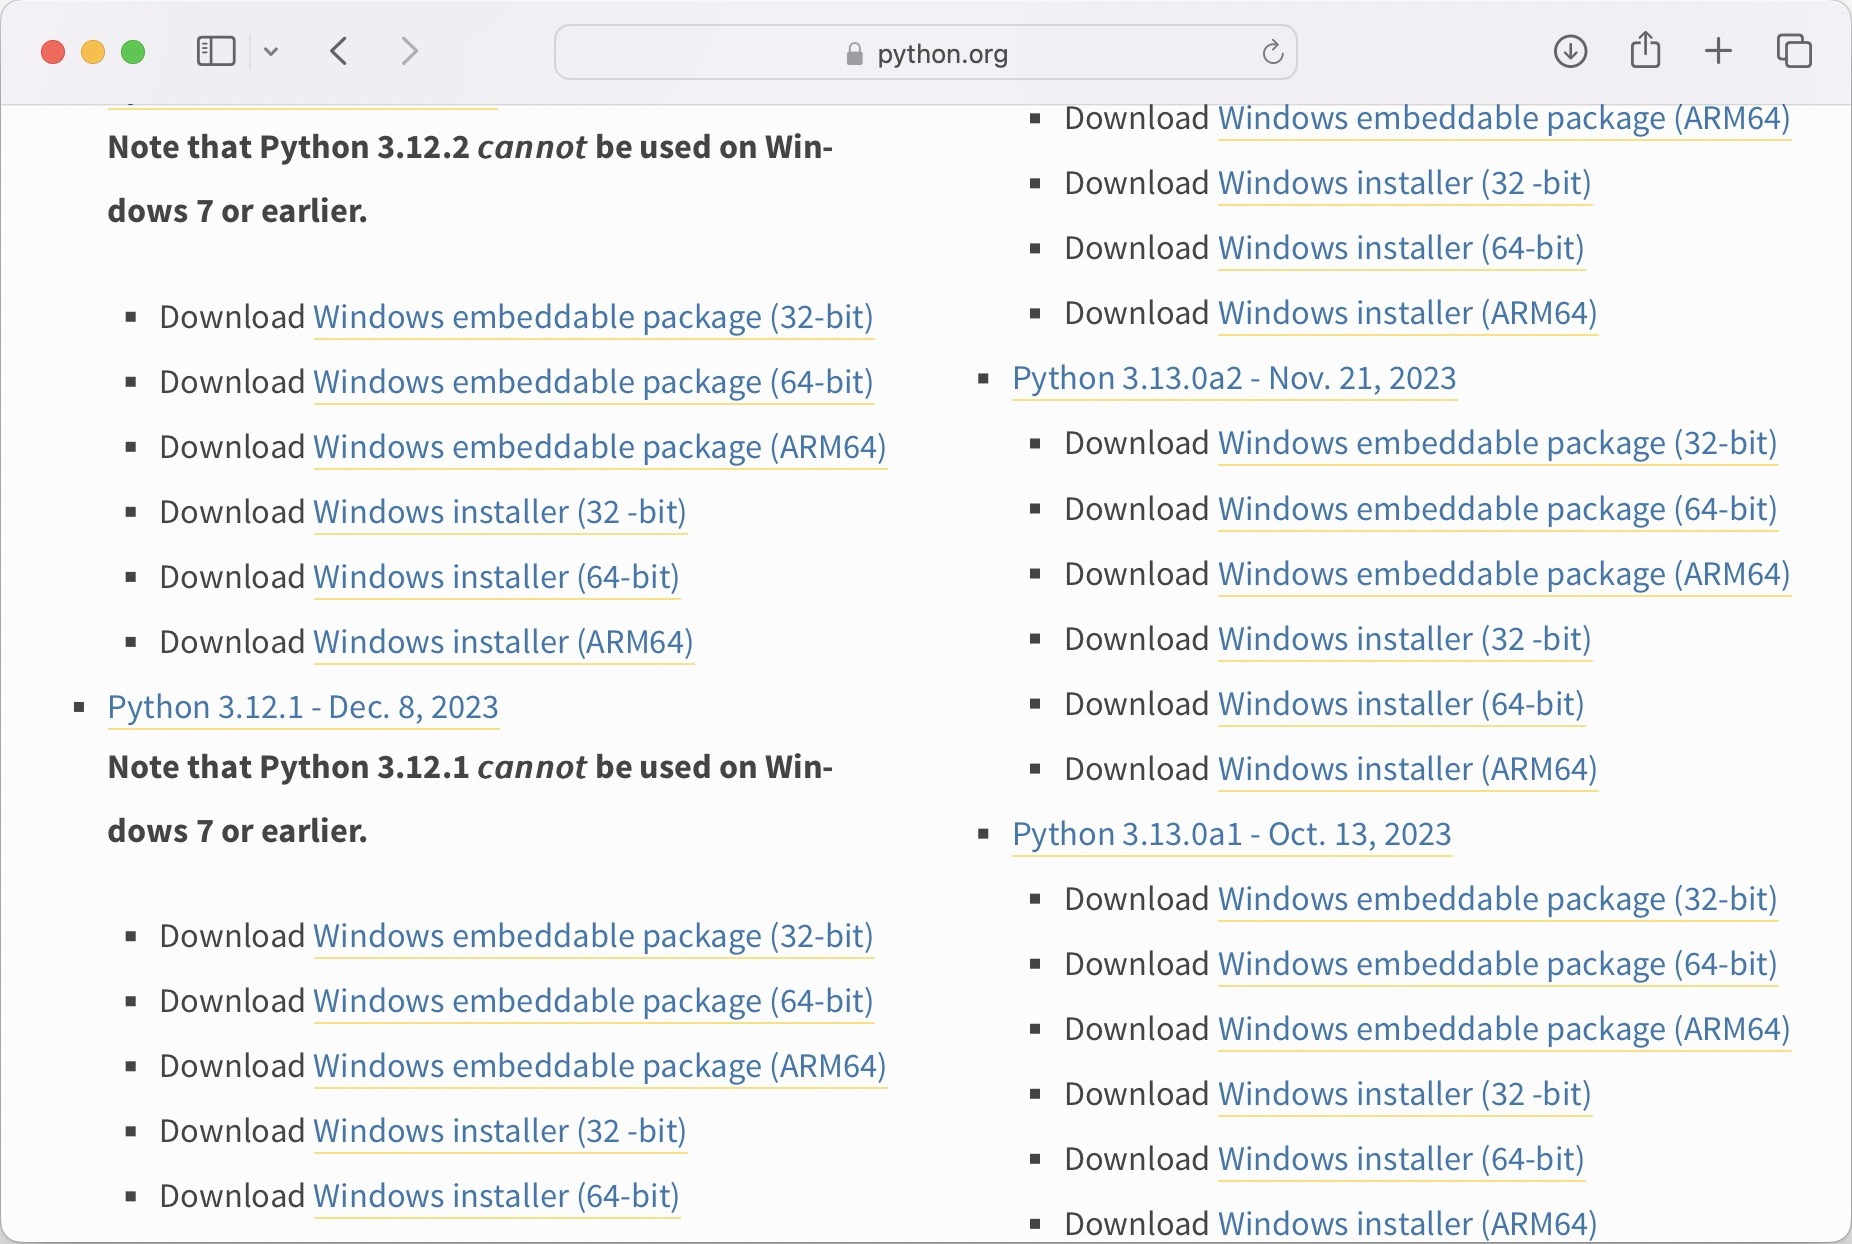
\includegraphics[width=.98\textwidth, trim={2.4mm 2mm 2mm 2mm},clip]{images/vscode_install/2.jpg}};
    \drawshadow{image}
    \draw [draw=red,very thick,rounded corners] (0.5,7) rectangle (6,7.78);
    \draw [draw=red,very thick,rounded corners] (0.75,4.38) rectangle (4.9,4.8);

\end{tikzpicture}
\caption{} 
\label{fig:pyvers}
\end{figure}

ဒေါင်းလုဒ်ပြီးရင် အင်စတော်လာဖိုင်ကို ညာကလစ်နှိပ်ပြီး \mytcboxinl{\fEnSnd{Run as administrator}} လုပ်ပါ။ ပုံ (\fRefNo{\ref{fig:pyinstlrun}}) ကိုကြည့်ပါ။ ပုံ (\fRefNo{\ref{fig:pyinstl1}}) မှာလို ဒိုင်ယာလော့ဂ် ဘောက်စ် ပွင့်လာပါမယ်။ အနီဝိုင်းထားတဲ့ ချက်ခ်ဘောက်စ်နှစ်ခုကို ချက်ခ်လုပ်ပြီး \mytcboxinl{\fEnSnd{Install Now}} နှိပ်ပါ။ အင်စတောလ် ပြီးလို့ \mytcboxinl{\fEnSnd{Setup was successful}} ပေါ်လာရင် \mytcboxinl{\fEnSnd{Close}} ခလုတ်နှိပ်ပြီး ပိတ်ပါ။

ဝင်းဒိုး \fEnSnd{command prompt (cmd)} မှာ \mytcboxinl{\fCode{python --version}} \fEn{run} ရင် ပုံ (\fRefNo{\ref{fig:pycmdchk}}) မှာလို အင်စတောလ်လုပ်ထားတဲ့ ဗားရှင်းကို ပြပေးသင့်ပါတယ်။
\begin{figure}[tbh!]
\begin{tikzpicture}
    \node[anchor=south west,inner sep=0] (image) at (0,0)
        {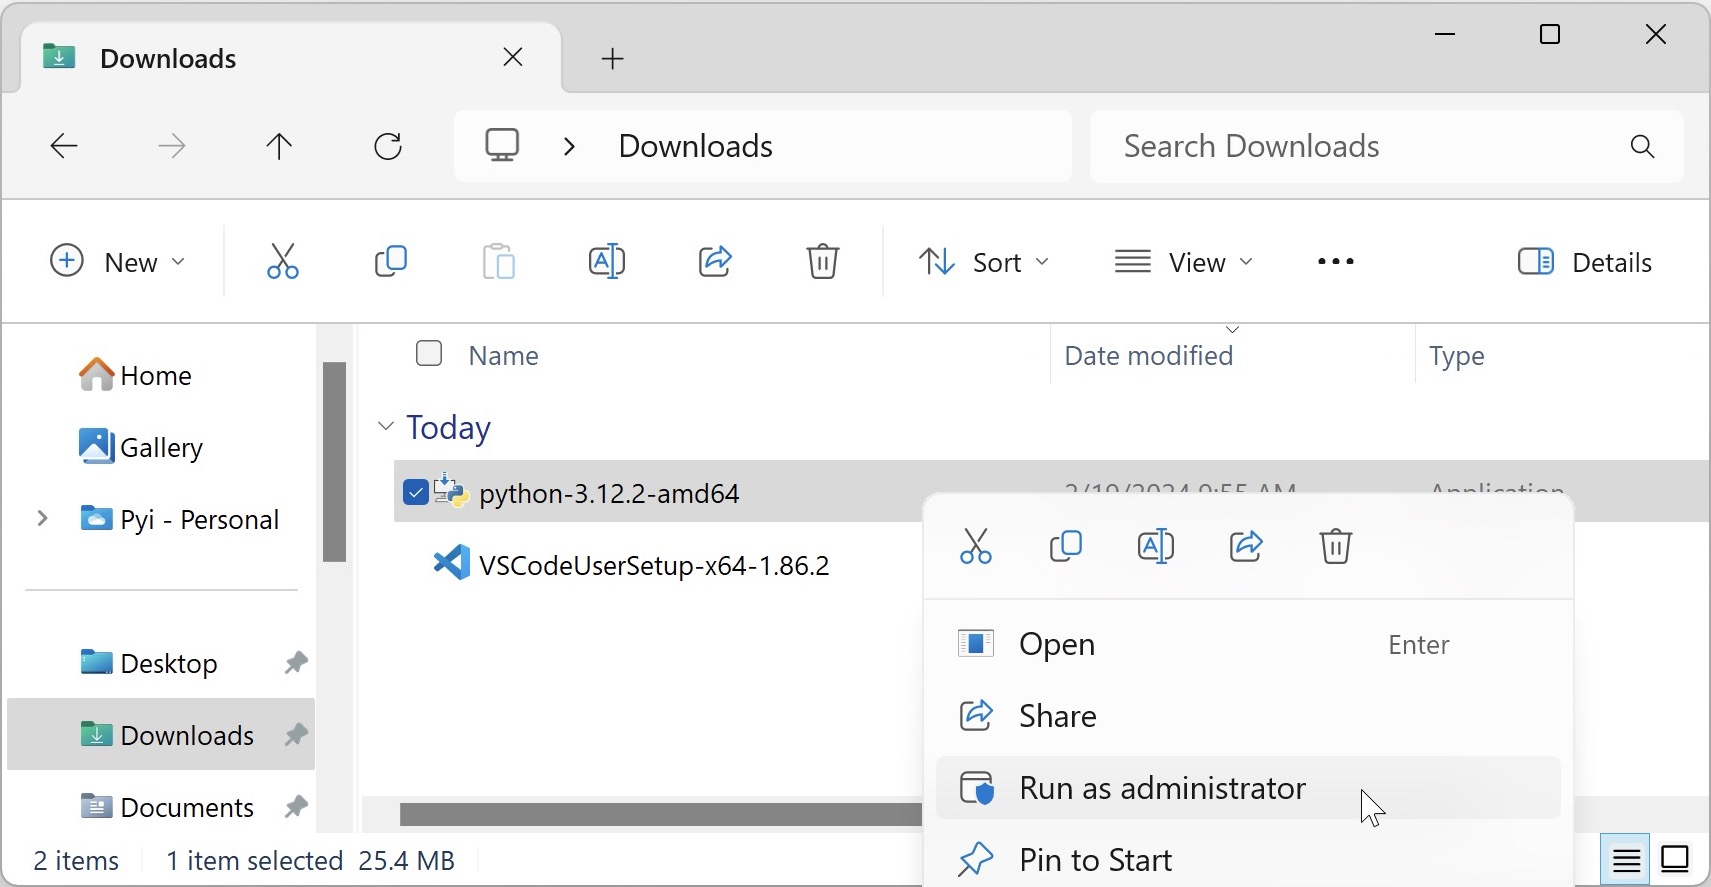
\includegraphics[width=.98\textwidth, trim={2.4mm 2mm 2mm 2mm},clip]{images/vscode_install/3.jpg}};
    \drawshadow{image}
\end{tikzpicture}
\caption{} 
\label{fig:pyinstlrun}
\end{figure}

\begin{figure}[tbh!]
\begin{tikzpicture}
    \node[anchor=south west,inner sep=0] (image) at (0,0)
        {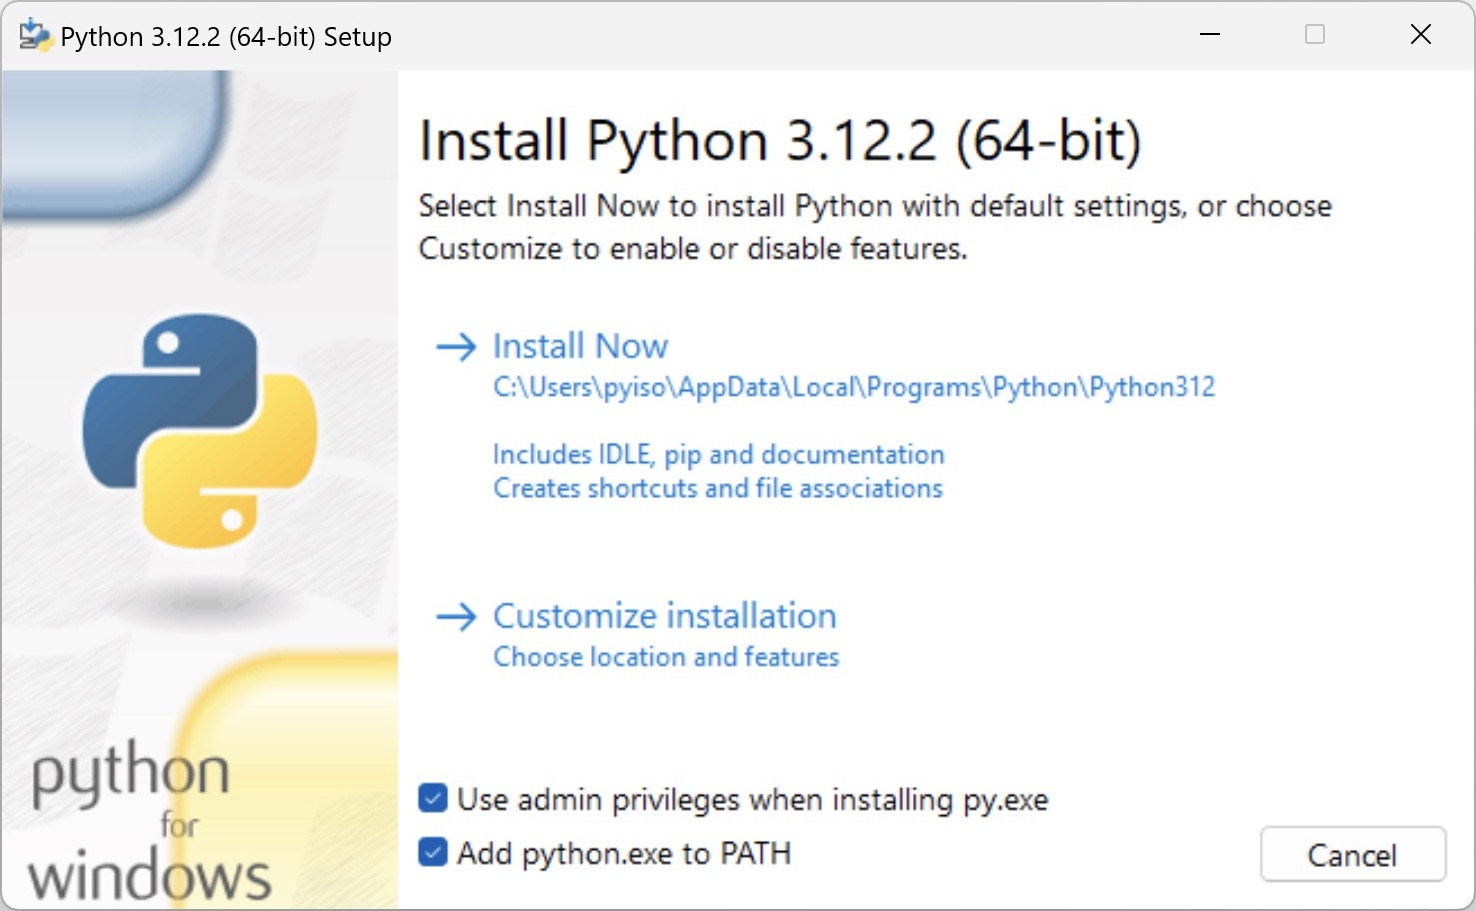
\includegraphics[width=.98\textwidth, trim={2.4mm 2mm 2mm 2mm},clip]{images/vscode_install/4.jpg}};
    \drawshadow{image}
    \draw [draw=red,very thick,rounded corners] (3.5,0.24) rectangle (9.25,1.15);
    \draw [draw=red, thick,rounded corners] (3.73,5.1) rectangle (10.75,4.35);
\end{tikzpicture}
\caption{} 
\label{fig:pyinstl1}
\end{figure}

\begin{figure}[tbh!]
\begin{tikzpicture}
    \node[anchor=south west,inner sep=0] (image) at (0,0)
        {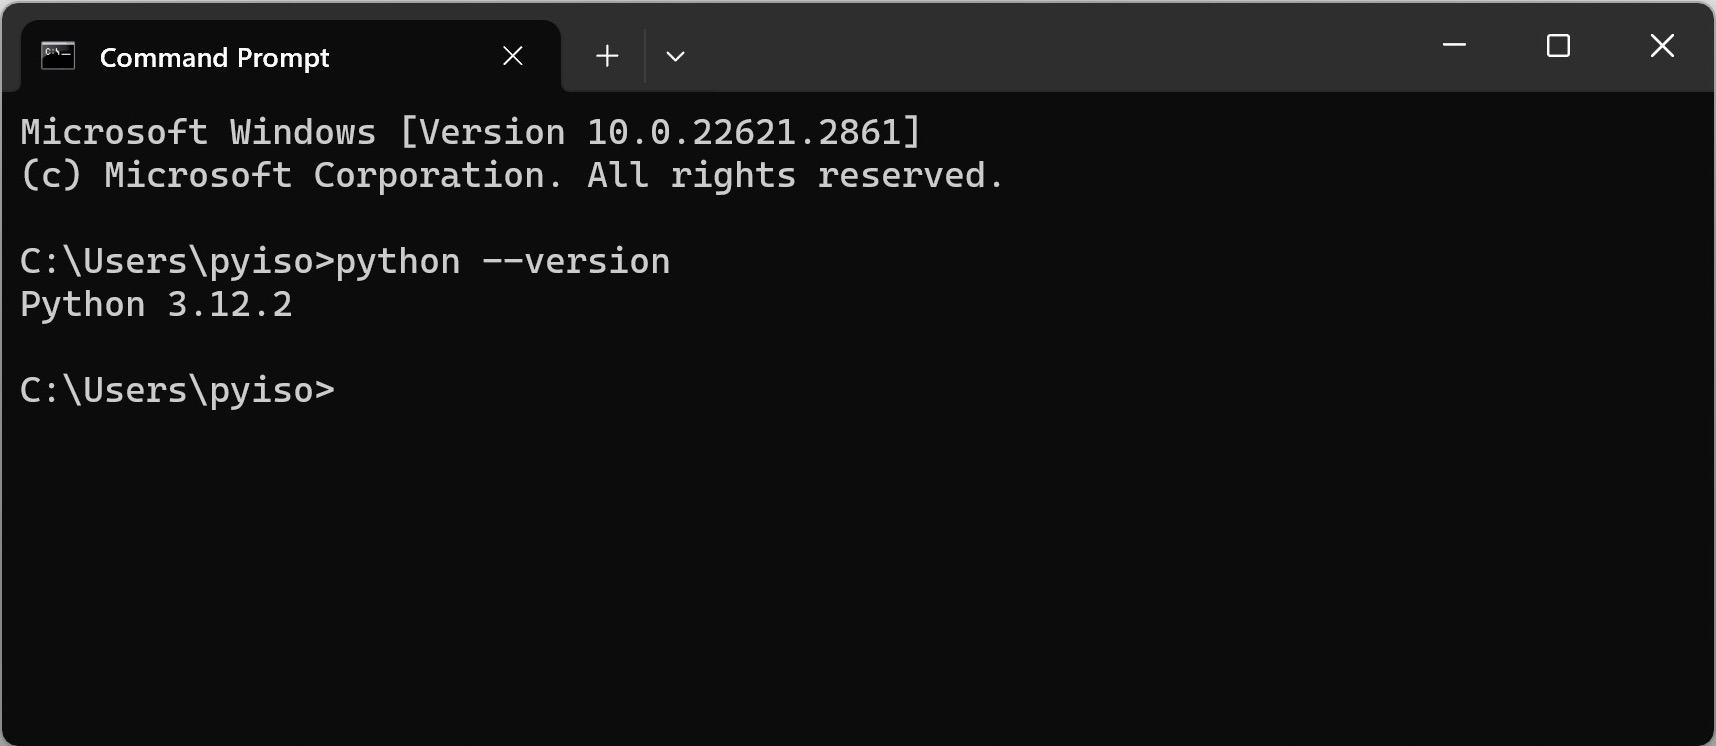
\includegraphics[width=.98\textwidth, trim={2.4mm 2mm 2mm 2mm},clip]{images/vscode_install/5.jpg}};
    \drawshadow{image}
\end{tikzpicture}
\caption{} 
\label{fig:pycmdchk}
\end{figure}

\clearpage
\subsection*{VS Code အင်စတောလ်လုပ်ခြင်း}\label{sec:vscode}
အခုဆိုရင် \fEn{Python programming language} အောင်မြင်စွာ ထည့်ပြီးသွားပါပြီ။ \fEn{VS Code} အင်စတောလ် ဆက်လုပ်ပါမယ်။ အင်စတာ်လာ ဒေါင်းလုဒ်လုပ်ရန် ဝဘ်စာမျက်နှာကို အောက်ပါလင့်
%
\begin{minted}[frame=lines, framerule=0pt]{text}
https://code.visualstudio.com 
\end{minted}
%
မှတစ်ဆင့် သွားပါ။ ပုံ (\fRefNo{\ref{fig:vsdwnpg}}) ဝဘ်စာမျက်နှာကို တွေ့ရပါမယ်။ \mytcboxinl{\fEnSnd{Download for Windows}} နှိပ်၍ ဒေါင်းလုဒ်လုပ်ပါ။

ပြီးတဲ့အခါ အင်စတော်လာဖိုင်ကို ညာကလစ်နှိပ်ပြီး ဖွင့်ပါ (ပုံ \fRefNo{\ref{fig:vsinstlropn}} မှာ ပြထားပါတယ်)။ အင်စတောလ် ဒိုင်ယာလော့ဂ်ဘောက်စ် ပွင့်လာရင် \mytcboxinl{\fEnSnd{I accept the agreement}} ကို ချက်ခ်လုပ်၍ \fEnSnd{Next>} တစ်ခုပြီးတစ်ခု ဆက်နှိပ်သွားပြီး နောက်ဆုံးမှာ  \fEnSnd{Install} နှိပ်ပါ။ အင်စတောလ်လုပ်နေတာကို ခဏစောင့်ပြီး၊ ပြီးသွားရင် \fEnSnd{Finish} နှိပ်ပါ။  

\fEn{Welcome} စခရင်ကို ပုံ (\fRefNo{\ref{fig:vswlcm}}) လို တွေ့ရပါမယ်။ \mytcboxinl{\fEnSnd{Dark Modern}} (သို့) \mytcboxinl{\fEnSnd{Light Modern}} နှစ်သက်ရာ သီးမ်စ် ရွေးပါ။ ဒါဆိုရင် \fEn{VS Code} လည်း အင်စတောလ် လုပ်ပြီးသွားပါပြီ။ ကားရဲလ်ပရိုဂရမ် ရေးဖို့ ဆက်လုပ်ရပါမယ်။

\begin{figure}[tbh!]
\begin{tikzpicture}
    \node[anchor=south west,inner sep=0] (image) at (0,0)
        {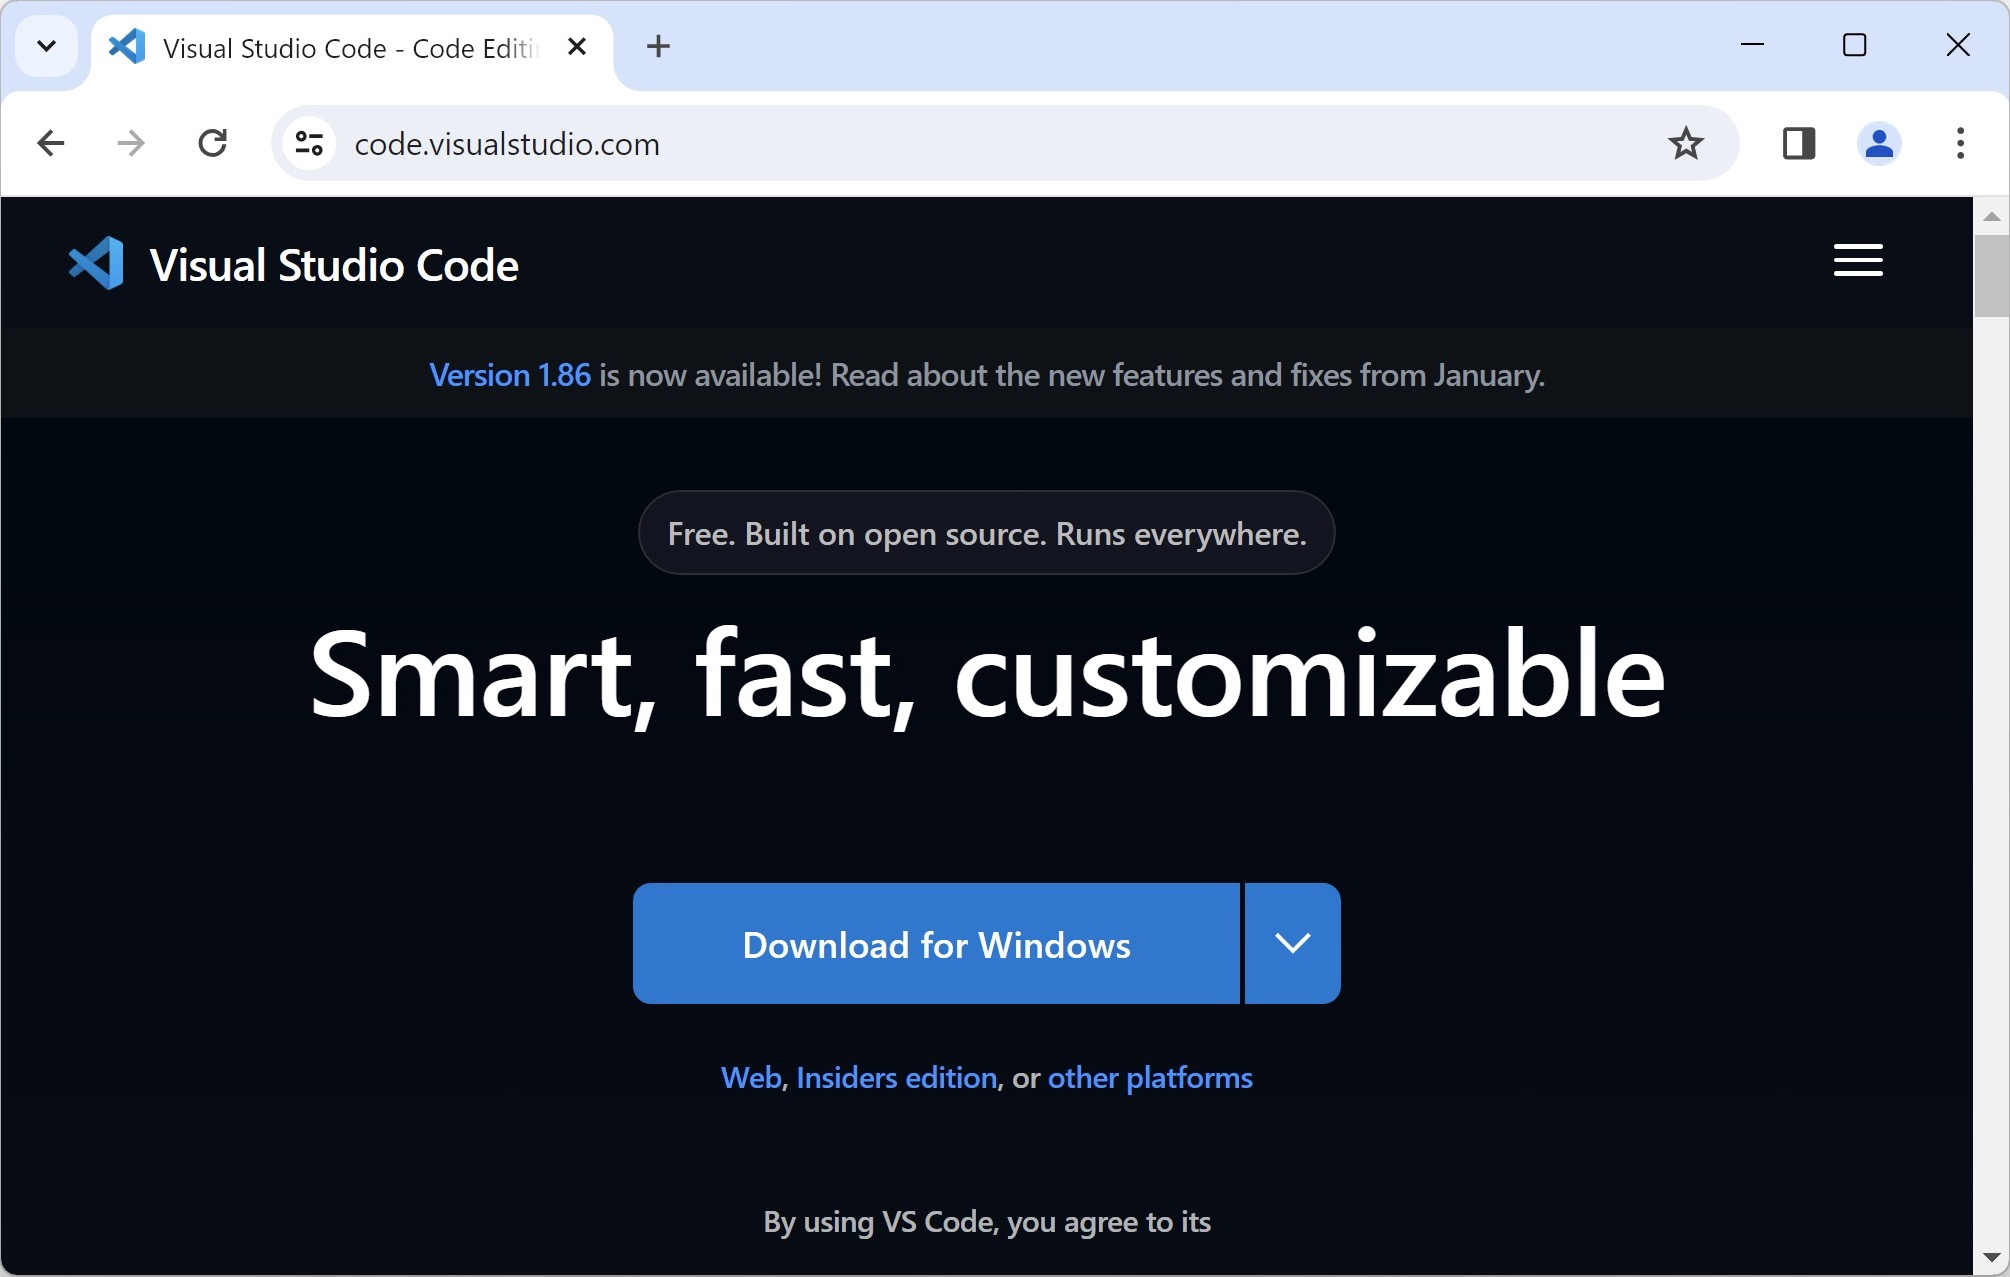
\includegraphics[width=.98\textwidth, trim={2.4mm 2cm 2mm 2mm},clip]{images/vscode_install/v0.jpg}};
    \drawshadow{image}
\end{tikzpicture}
\caption{} 
\label{fig:vsdwnpg}
\end{figure}

\begin{figure}[tbh!]
\begin{tikzpicture}
    \node[anchor=south west,inner sep=0] (image) at (0,0)
        {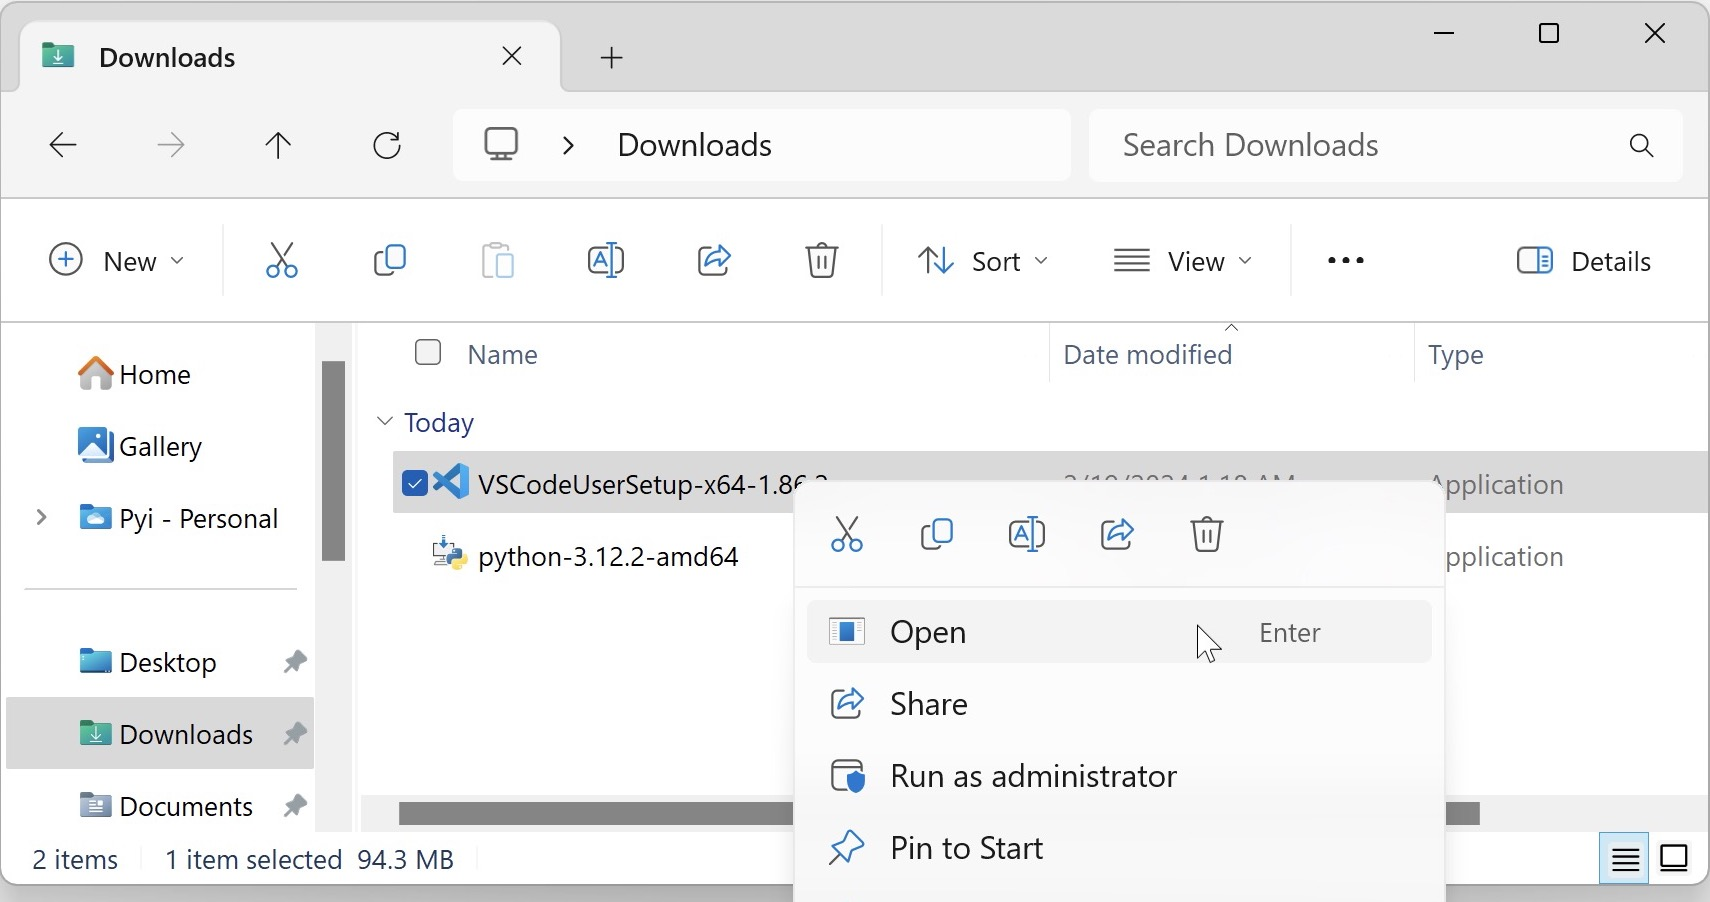
\includegraphics[width=.98\textwidth, trim={2.4mm 2mm 2mm 2mm},clip]{images/vscode_install/v1.jpg}};
    \drawshadow{image}
\end{tikzpicture}
\caption{} 
\label{fig:vsinstlropn}
\end{figure}

\begin{figure}[tbh!]
\begin{tikzpicture}
    \node[anchor=south west,inner sep=0] (image) at (0,0)
        {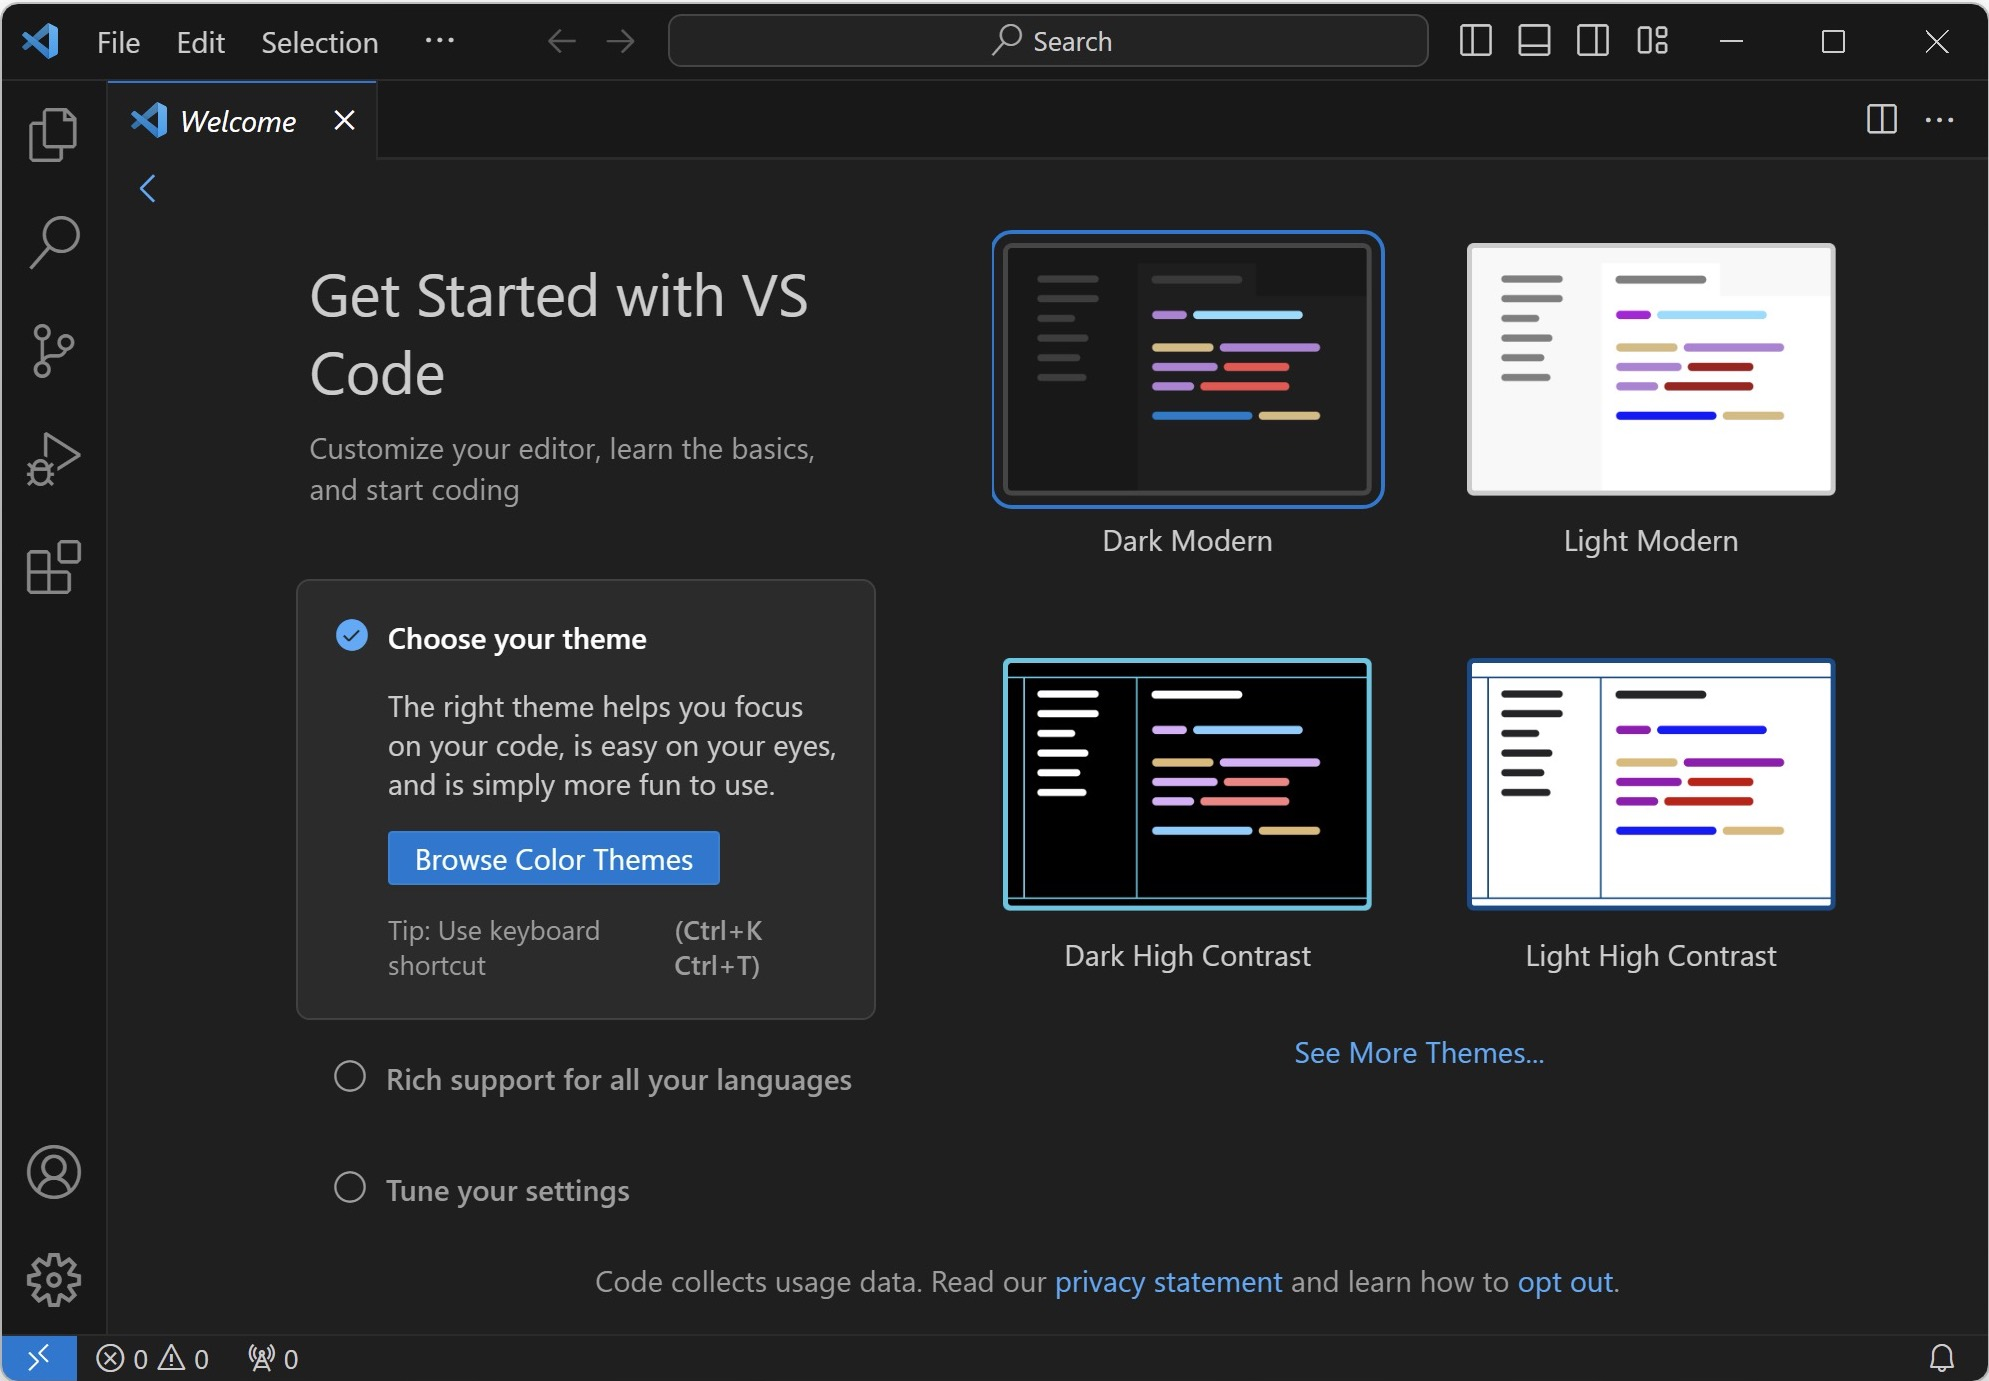
\includegraphics[width=.98\textwidth, trim={2.4mm 2mm 2mm 2mm},clip]{images/vscode_install/v1b.jpg}};
    \drawshadow{image}
    
    \draw [draw=red,very thick,rounded corners] (6.25,7.5) rectangle (9.08,5.25);
    \draw [draw=red,very thick,rounded corners] (9.35,7.5) rectangle (12.01,5.25);
    \draw [draw=red,very thick,rounded corners] (0.08,5.5) rectangle (0.6,5);
\end{tikzpicture}
\caption{} 
\label{fig:vswlcm}
\end{figure}

\clearpage

\subsection*{VS Code Python Extension ထည့်ခြင်း}
\fEn{Python} ပရိုဂရမ်ရေးဖို့အတွက် \fEn{VS Code} က ဒီအတိုင်းဆိုရင် သိပ်အဆင်မပြေသေးပါဘူး။ \fEn{Python} အတွက် \fEn{extension} အင်စတောလ် လုပ်ပေးရပါအုံးမယ်။ ပုံ (\fRefNo{\ref{fig:vswlcm}}) ဘယ်ဘက်ဘောင်နားမှာ အနီဝိုင်းထားတဲ့ အိုင်ကွန်လေးကို နှိပ်ပါ။ \fEn{Python} \fEnSnd{extension} ကိုရှာပါ။   ပုံ (\fRefNo{\ref{fig:vspyplugin1}}) မှာ ဘယ်လိုရှာရမလဲ ပြထားပါတယ်။ ပုံမှာတွေ့ရတဲ့ \fEn{Microsoft} က ထုတ်တဲ့ \fEnSnd{extension} ကို အင်စတောလ်လုပ်ပါ။ အောင်မြင်ရင် ပုံ (\fRefNo{\ref{fig:vspyplugin2}}) မှာလို ဖြစ်သွားပါမယ်။ \fEn{Python} နဲ့  \fEn{VS Code} ကိစ္စတော့ ပြီးသွားပြီ။ ကားရဲလ် \fEn{example} \fEn{run} ဖို့ ဆက်လုပ်ရမယ်။
\begin{figure}[tbh!]
\begin{tikzpicture}
    \node[anchor=south west,inner sep=0] (image) at (0,0)
        {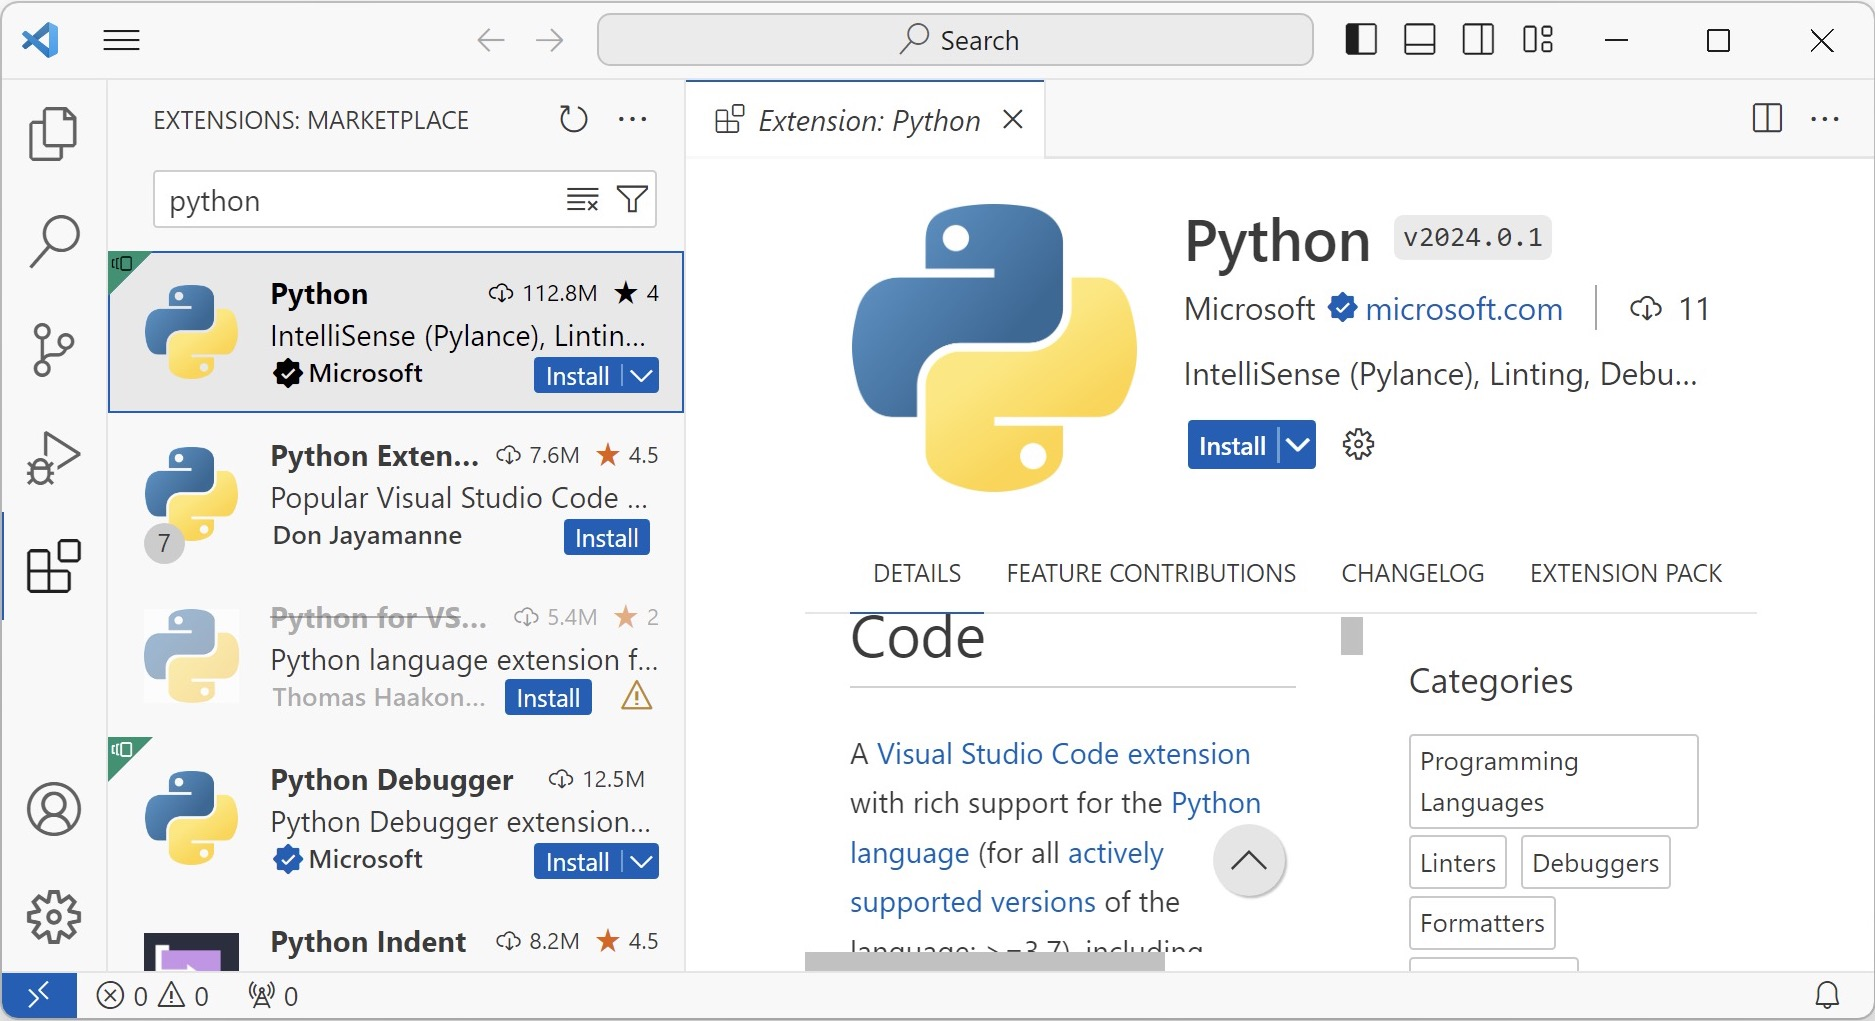
\includegraphics[width=.98\textwidth, trim={2.4mm 2mm 2mm 2mm},clip]{images/vscode_install/v2.jpg}};
    \drawshadow{image}
\end{tikzpicture}
\caption{} 
\label{fig:vspyplugin1}
\end{figure}

\begin{figure}[tbh!]
\begin{tikzpicture}
    \node[anchor=south west,inner sep=0] (image) at (0,0)
        {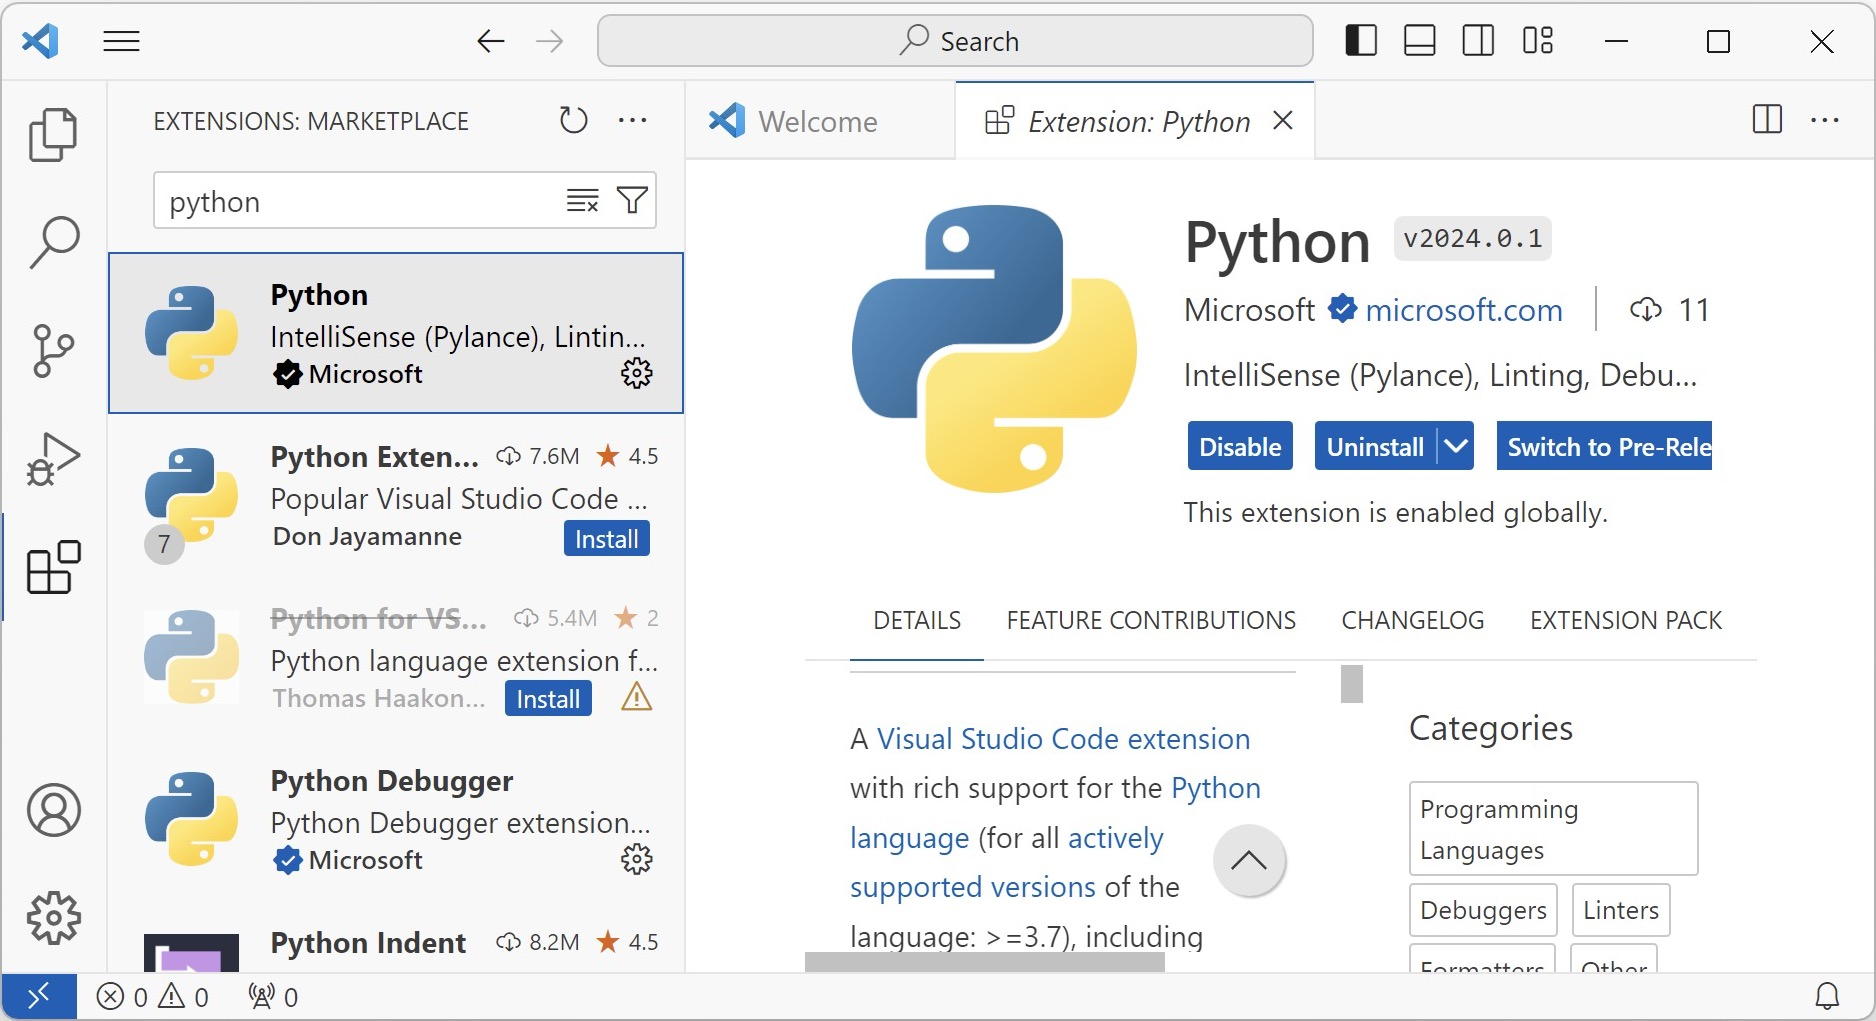
\includegraphics[width=.98\textwidth, trim={2.4mm 2mm 2mm 2mm},clip]{images/vscode_install/v3.jpg}};
    \drawshadow{image}
\end{tikzpicture}
\caption{} 
\label{fig:vspyplugin2}
\end{figure}

\clearpage

\subsection*{နမူနာ ကားရဲလ် ကမ္ဘာနှင့် ပရိုဂရမ်ကုဒ် ဖိုင်များထည့်ခြင်း}
\fEnSnd{meet\_karel.zip} ဖိုင်ကို \todo{ဒေါင်းလုဒ်လင့်ထည့်ရန်} ဒီလင့် \fCode{http://tinyurl.com/3mmm9c7j} ကနေ ဒေါင်းလုဒ်လုပ်ပါ။ ၎င်း \fEnSnd{zip} ဖိုင်ကို \fEn{extract} လုပ်ပါ။ \fEnSnd{meet\_karel} နံမည်နဲ့ ဖိုဒါတစ်ခု ရလာပါမယ်။ ဖိုဒါထဲ ဝင်ကြည့်ရင် အောက်ပါအတိုင်း ရှိသင့်ပါတယ်။ 
%
\begin{itemize}
    \item \fEnSnd{worlds} 
    \begin{itemize}
        \item \fEnSnd{meet\_karel.w}
        \item \fEnSnd{move\_beeper\_to\_other\_side.w}
    \end{itemize}
    \item \fEnSnd{meet\_karel.py}
    \item \fEnSnd{move\_beeper\_to\_other\_side.py}
    \item \fEnSnd{world\_editor.py}
\end{itemize}
%

\begin{figure}[tbh!]
\begin{tikzpicture}
    \node[anchor=south west,inner sep=0] (image) at (0,0)
        {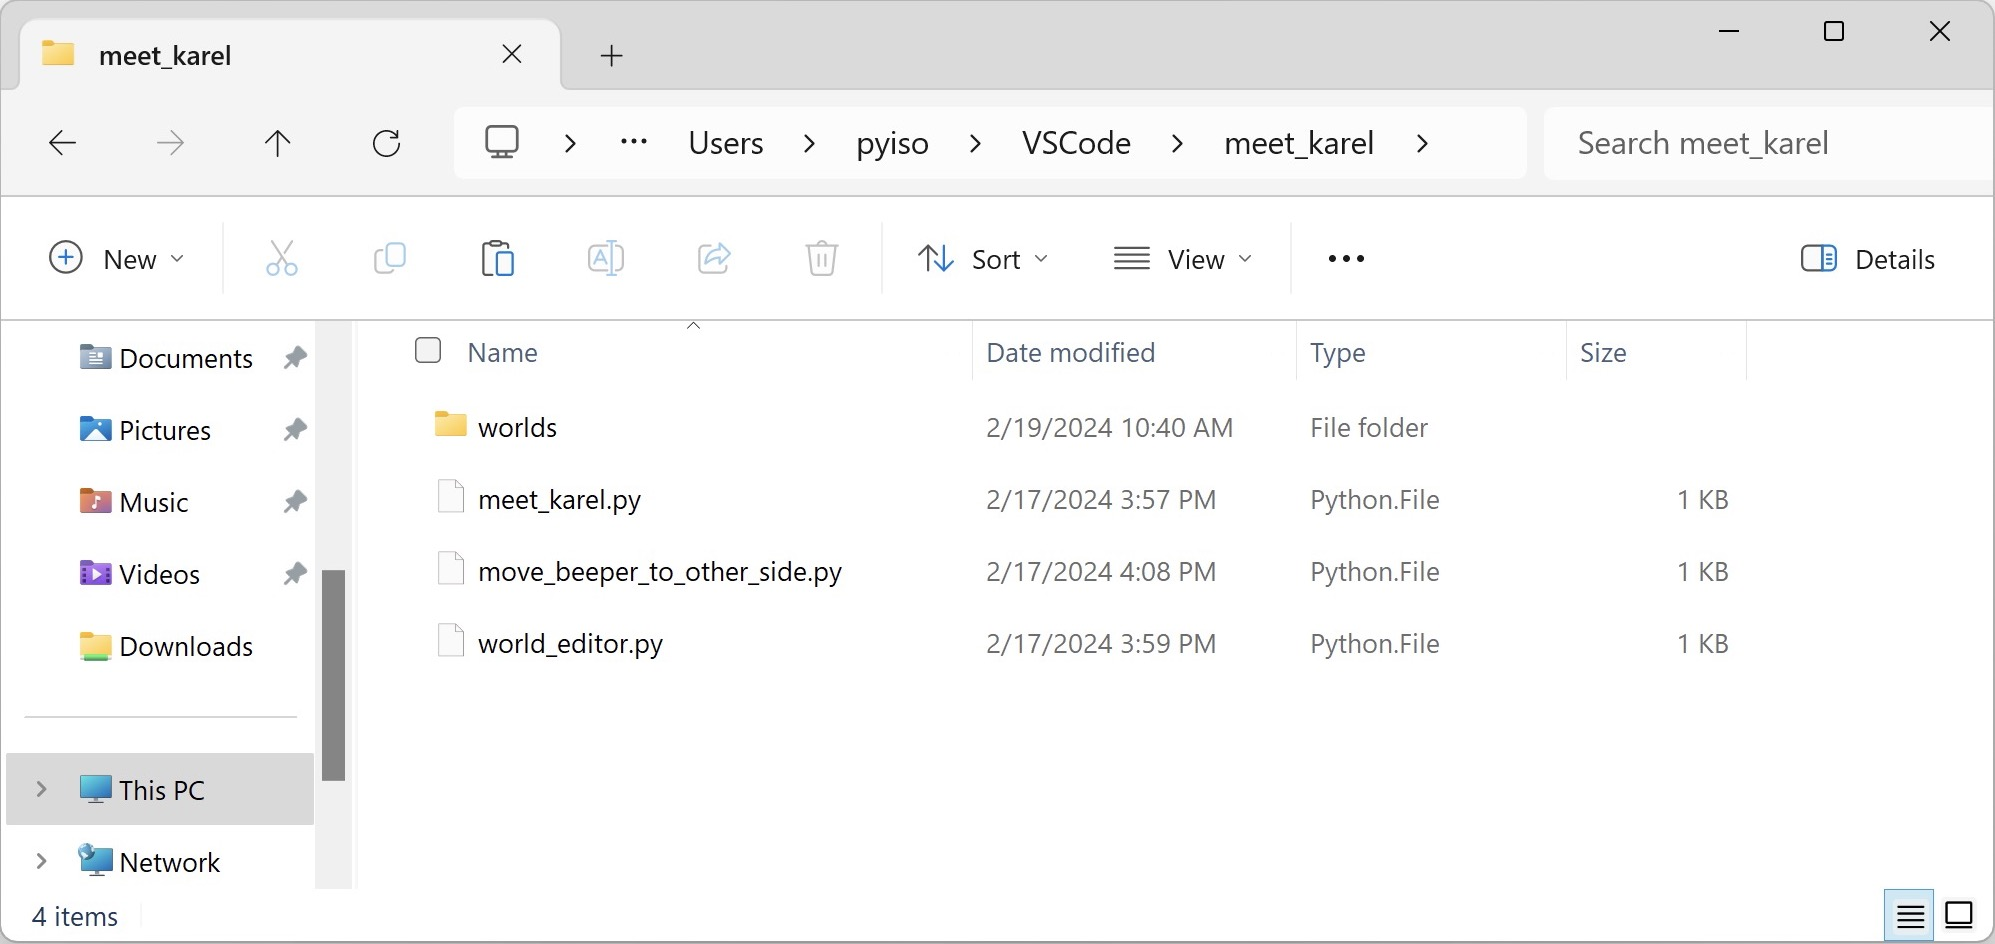
\includegraphics[width=.98\textwidth, trim={2.4mm 2mm 2mm 2mm},clip]{images/vscode_install/v4.jpg}};
    \drawshadow{image}
\end{tikzpicture}
\caption{} 
\label{fig:mtkrl1}
\end{figure}

\begin{figure}[tbh!]
\begin{tikzpicture}
    \node[anchor=south west,inner sep=0] (image) at (0,0)
        {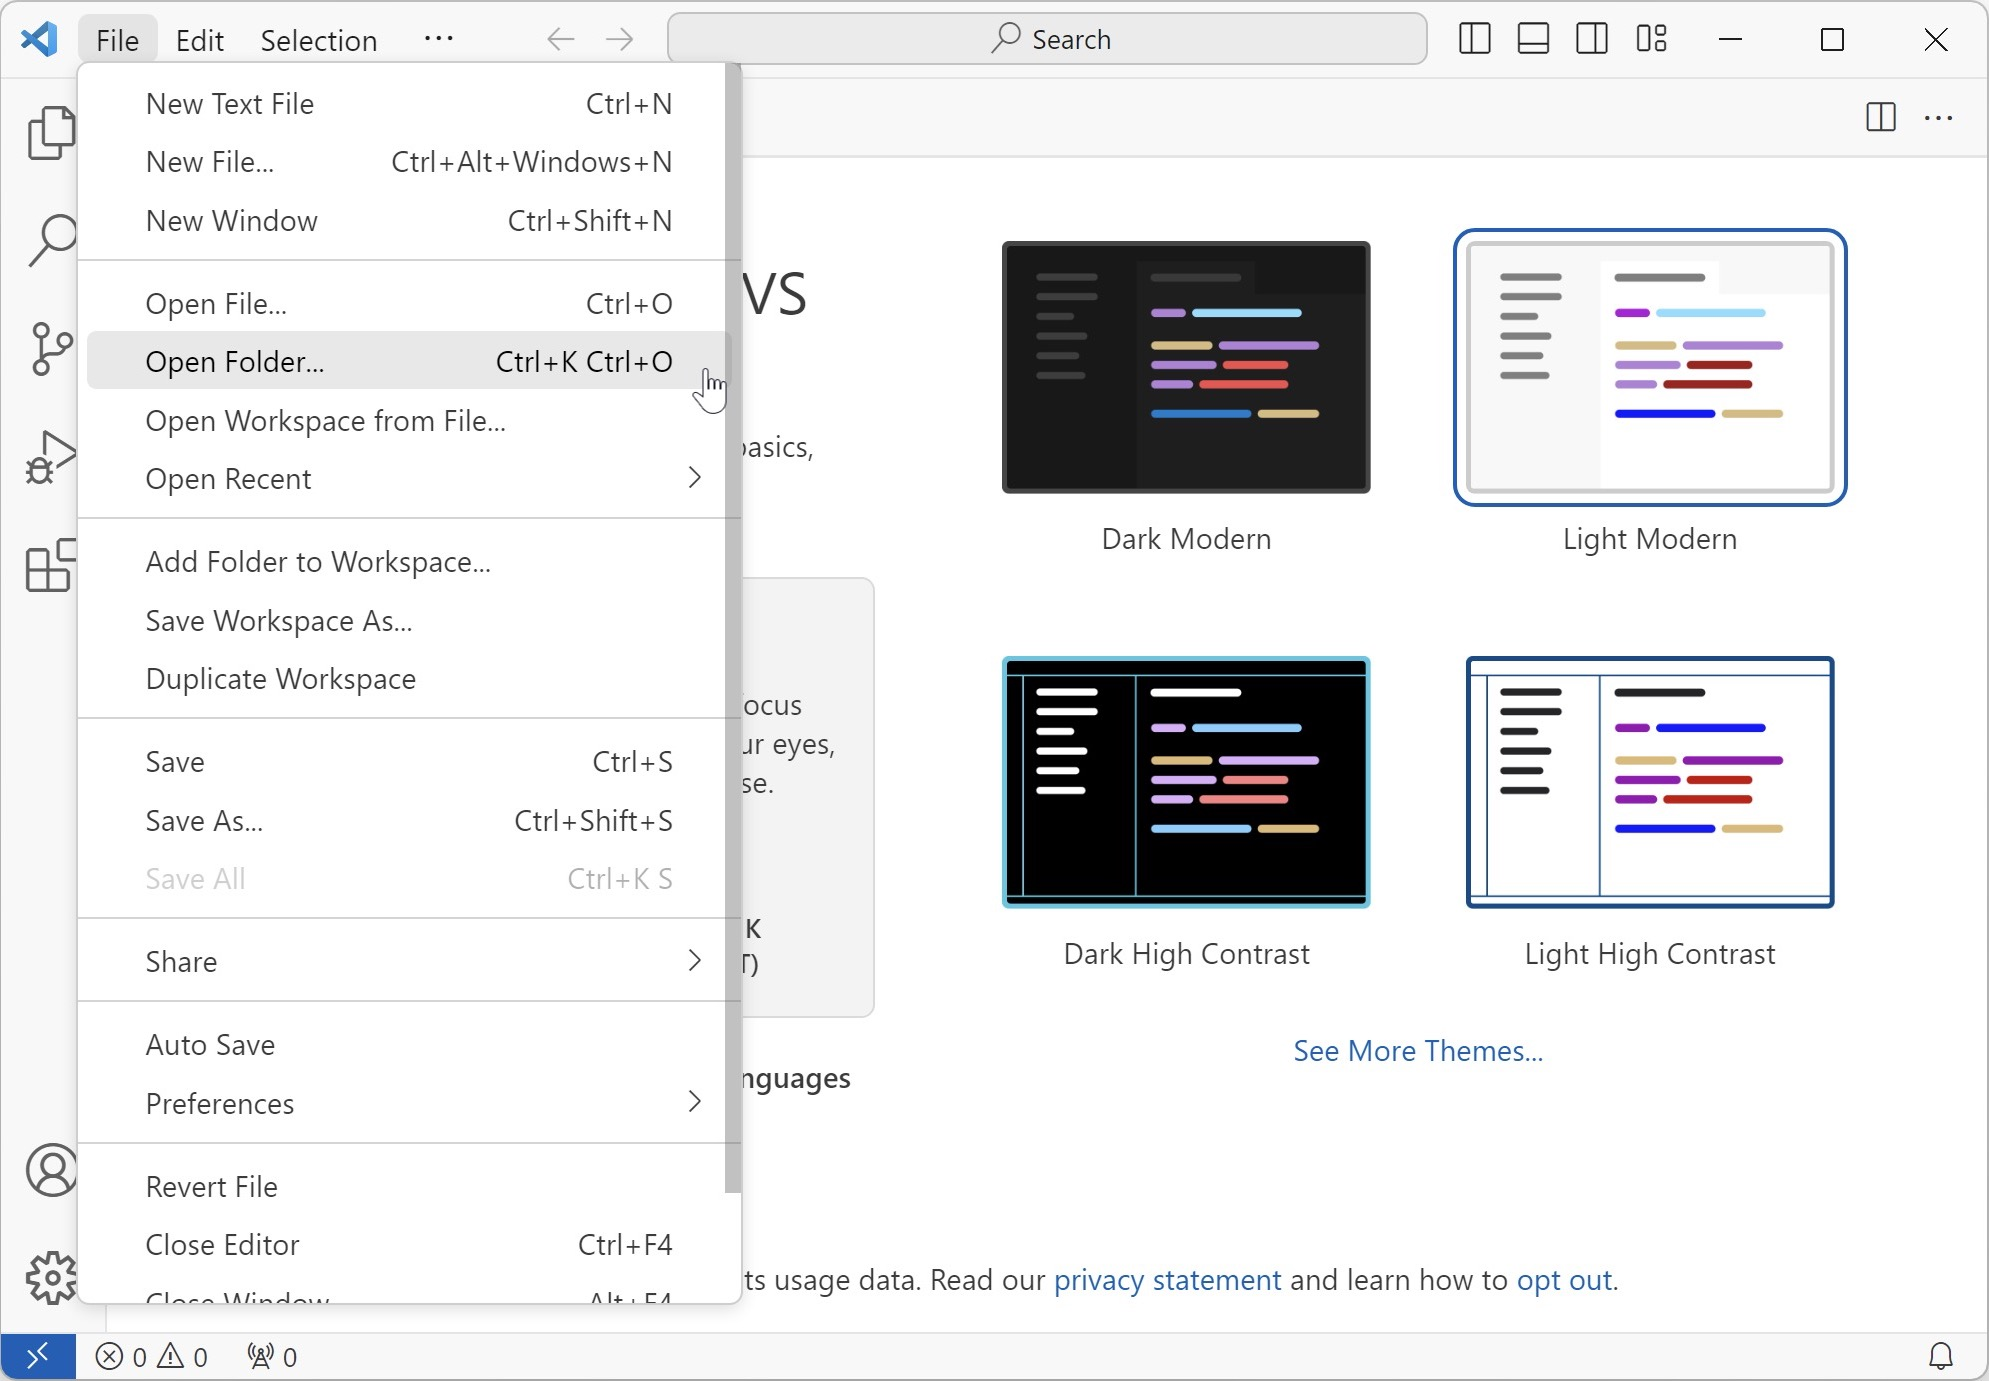
\includegraphics[width=.98\textwidth, trim={2.4mm 2mm 2mm 2mm},clip]{images/vscode_install/v5b.jpg}};
    \drawshadow{image}
\end{tikzpicture}
\caption{} 
\label{fig:opnmtkrl}
\end{figure}

\begin{figure}[tbh!]
\begin{tikzpicture}
    \node[anchor=south west,inner sep=0] (image) at (0,0)
        {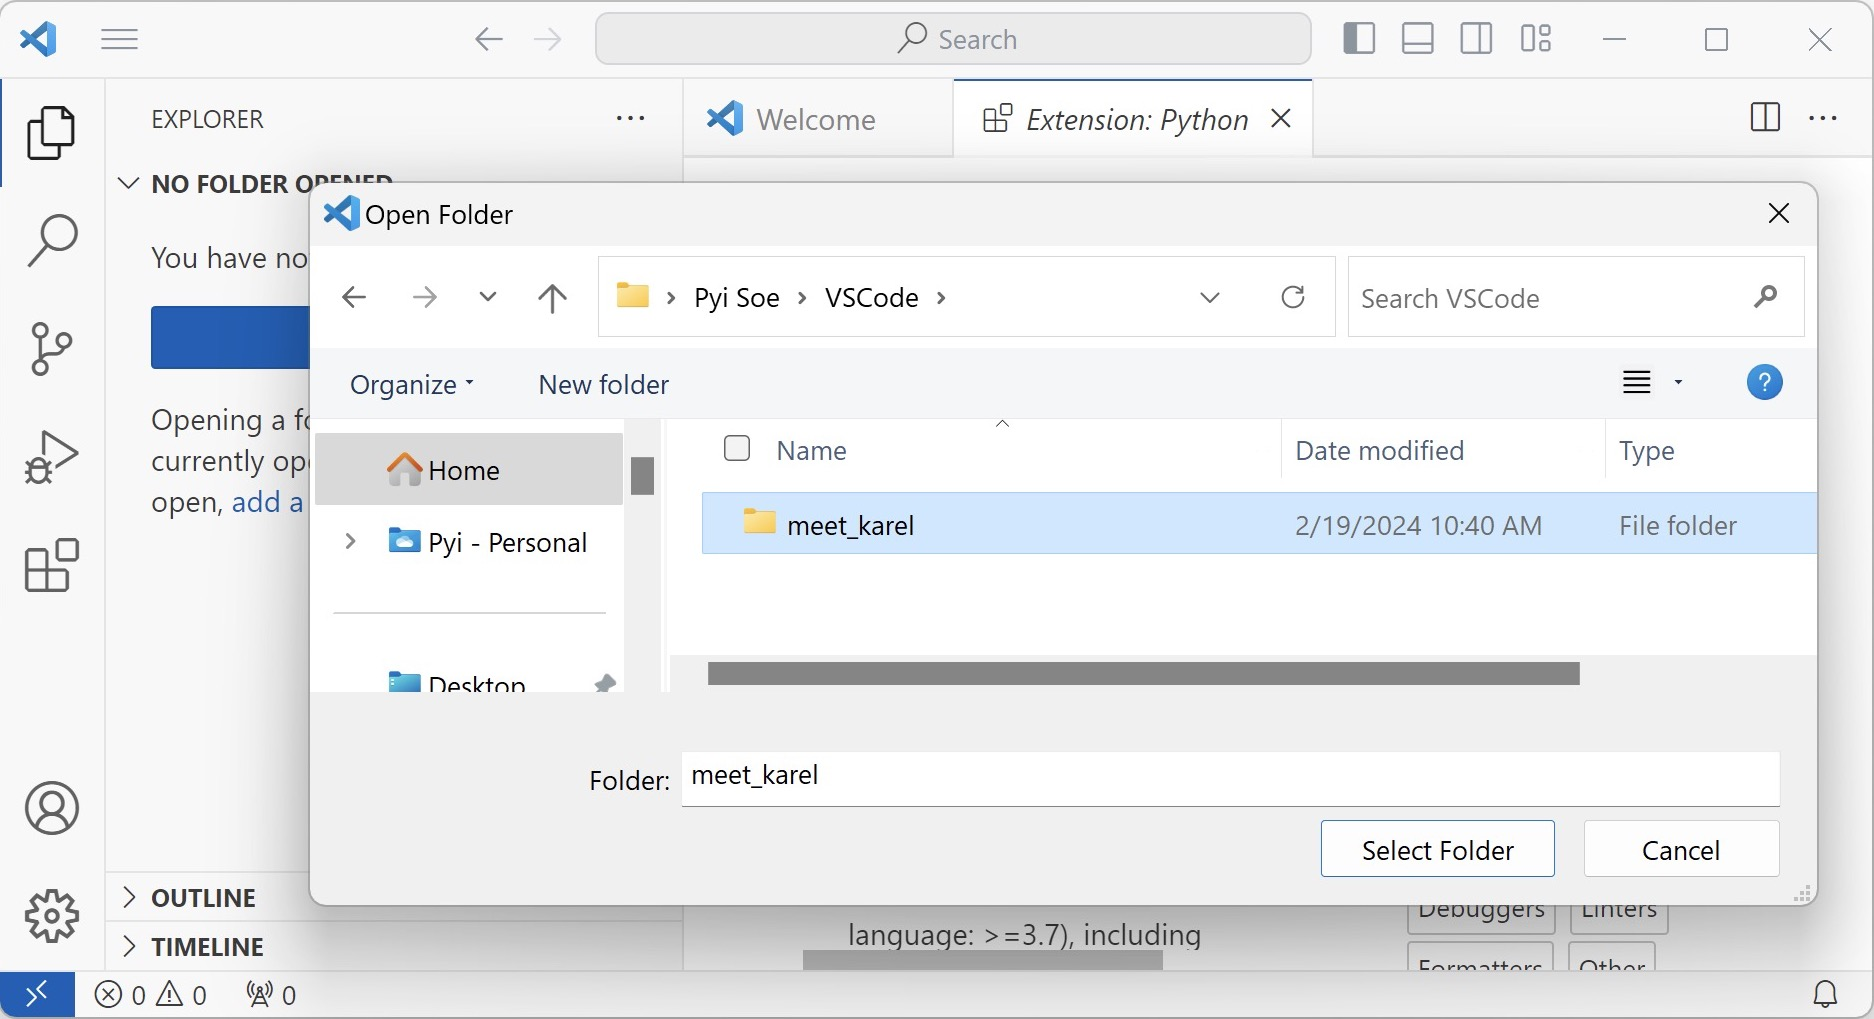
\includegraphics[width=.98\textwidth, trim={2.4mm 2mm 2mm 2mm},clip]{images/vscode_install/v6.jpg}};
    \drawshadow{image}
\end{tikzpicture}
\caption{} 
\label{fig:mtkrl3}
\end{figure}

\fEn{VS Code} အတွက် ဖိုဒါတစ်ခုကို မိမိအတွက် အဆင်ပြေမဲ့နေရာမှာ သီးသန့်တည်ဆောက် ထားသင့်တယ်။ ဥပမာ 
%
\begin{minted}[frame=lines, framerule=0pt,escapeinside=ßß]{text}
ß\fEnSnd{C:{\textbackslash}Users{\textbackslash}\textit{yourname}{\textbackslash}VS Code}ß
\end{minted}
%
\begin{mytcbox}
မိမိ လက်ရှိ \fEn{Home} ဖိုဒါကို  \mytcboxinl{\fEnSnd{C:}} \fEn{drive} ရဲ့ \mytcboxinl{\fEnSnd{Users}}  ဖိုဒါထဲမှာ တွေ့နိုင်ပါတယ်။ \mytcboxinl{\fEnSnd{Win + R}} ရှော့ကတ်နှိပ်ပြီး \mintinline{text}|%userprofile%| ရိုက်ထည့်၊ \fEnSnd{Ok} လုပ်ပြီး \fEn{Home} ဖိုဒါကို သွားနိုင်ပါတယ်။ အကယ်၍ မသွားတတ်ရင်လည်း ပြဿနာမရှိပါဘူး။ ကိုယ့်အတွက် လွယ်ကူမဲ့ \fEnSnd{Desktop, Downloads, Documents} တစ်ခုခုထဲမှာ \fEn{VS Code} အတွက် ဖိုဒါတစ်ခု ထားလည်းရတယ်။
\end{mytcbox}

\mytcboxinl{\fEnSnd{meet\_karel}} ဖိုဒါ (\fEnSnd{.zip} ဖိုင်မဟုတ်ပါ) ကို အထက်ပါအတိုင်း အသစ် ဆောက်ထားတဲ့ \fEn{VS Code} သီးသန့်ဖိုဒါထဲကို ကော်ပီကူးထည့်ပါ။ ၎င်း \mytcboxinl{\fEnSnd{meet\_karel}} ဖိုဒါကို \fEn{VS Code} \mytcboxinl{\fEnSnd{File}} မီနူးမှ \mytcboxinl{\fEnSnd{Open Folder}} နှိပ်၍ ဖွင့်ပါ။ ပုံ (\fRefNo{\ref{fig:opnmtkrl}}) တွင်ကြည့်ပါ။

အခန်းအလိုက် နမူနာ ကုဒ်ဖိုင်တွေ ထည့်ပေးထားတဲ့ \fEnSnd{.zip} ဖိုင်တွေကိုလည်း အထက်ပါအတိုင်း လုပ်ရပါမယ်။ \fEnSnd{.zip} ဖိုင်ကို ဖြည်၊ ရလာတဲ့ ဖိုဒါကို သီးသန့်ဖိုဒါတစ်ခုထဲကို ကော်ပီကူးထည့်၊ \fEn{VS Code} နဲ့ အဲ့ဒီဖိုဒါကို ဖွင့်ရုံပါပဲ။



\clearpage
\subsection*{stanfordkarel လိုက်ဘရီ အင်စတောလ်လုပ်ခြင်း}
\mytcboxinl{\fEnSnd{meet\_karel.py}} ဖိုင်ကို ကလစ်နှစ်ချက်နှိပ် ဖွင့်ပါ။ ကုဒ်အယ်ဒီတာ ပွင့်လာမယ် (ပုံ \fRefNo{\ref{fig:edtmtkrl}})။ အဲဒီ ကုဒ်အယ်ဒီတာပေါ် (သို့) \mytcboxinl{\fEnSnd{meet\_karel.py}} ဖိုင်ကို ညာကလစ်နှိပ်ပြီး \mytcboxinl{\fEnSnd{Run Python File in Terminal}} လုပ်ပါ (ပုံ \fRefNo{\ref{fig:runmtkrl2}})။ \fEnSnd{Terminal} ပွင့်လာပြီး အယ်ရာ\fOpn{မက်ဆေ့ချ်}တွေ ပြလိမ့်မယ်။ ပုံ (\fRefNo{\ref{fig:mtkrlfstrun}}) မှာကြည့်ပါ။ ကားရဲလ်ပရိုဂရမ်အတွက် လိုအပ်တဲ့ \fEnSnd{stanfordkarel} လိုက်ဘရီ အင်စတောလ် မလုပ်ရသေးပါဘူး။ ဒါကြောင့် အယ်ရာဖြစ်နေတာ။

\begin{figure}[tbh!]
\begin{tikzpicture}
    \node[anchor=south west,inner sep=0] (image) at (0,0)
        {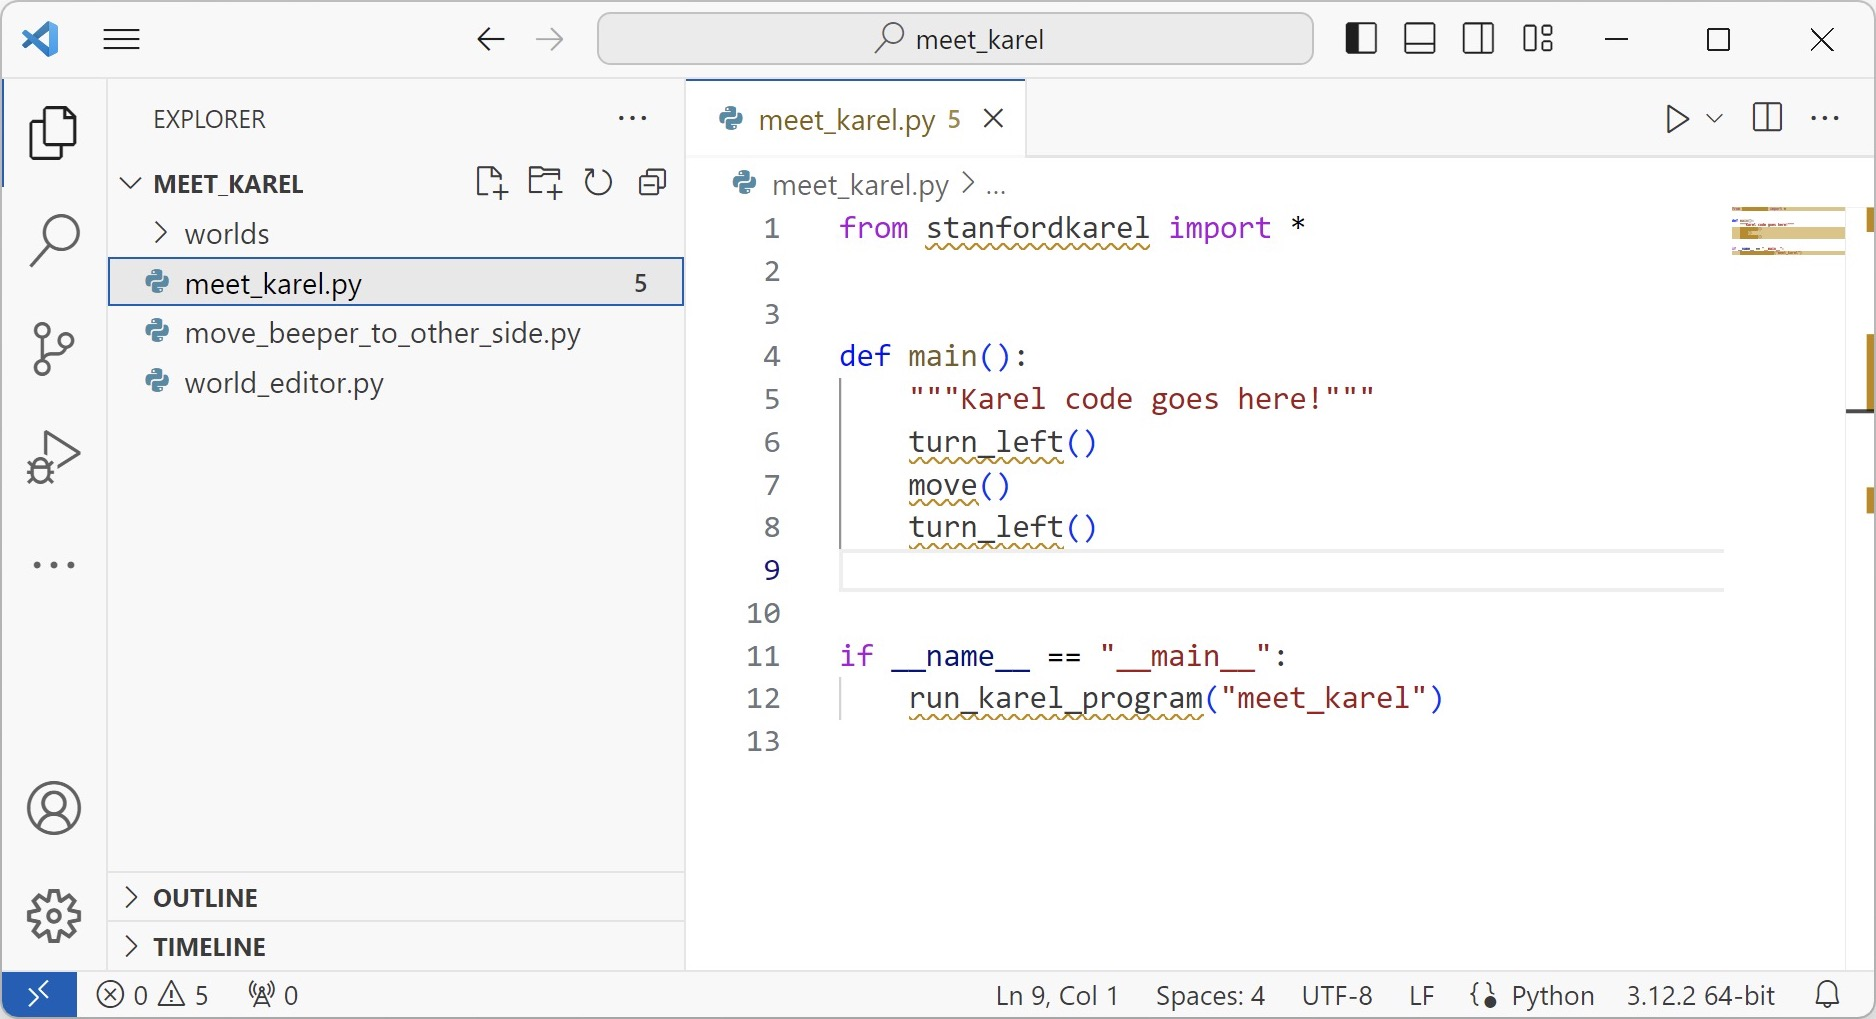
\includegraphics[width=.98\textwidth, trim={2.4mm 2mm 2mm 2mm},clip]{images/vscode_install/v7.jpg}};
    \drawshadow{image}
\end{tikzpicture}
\caption{} 
\label{fig:edtmtkrl}
\end{figure}

\begin{figure}[tbh!]
\begin{tikzpicture}
    \node[anchor=south west,inner sep=0] (image) at (0,0)
        {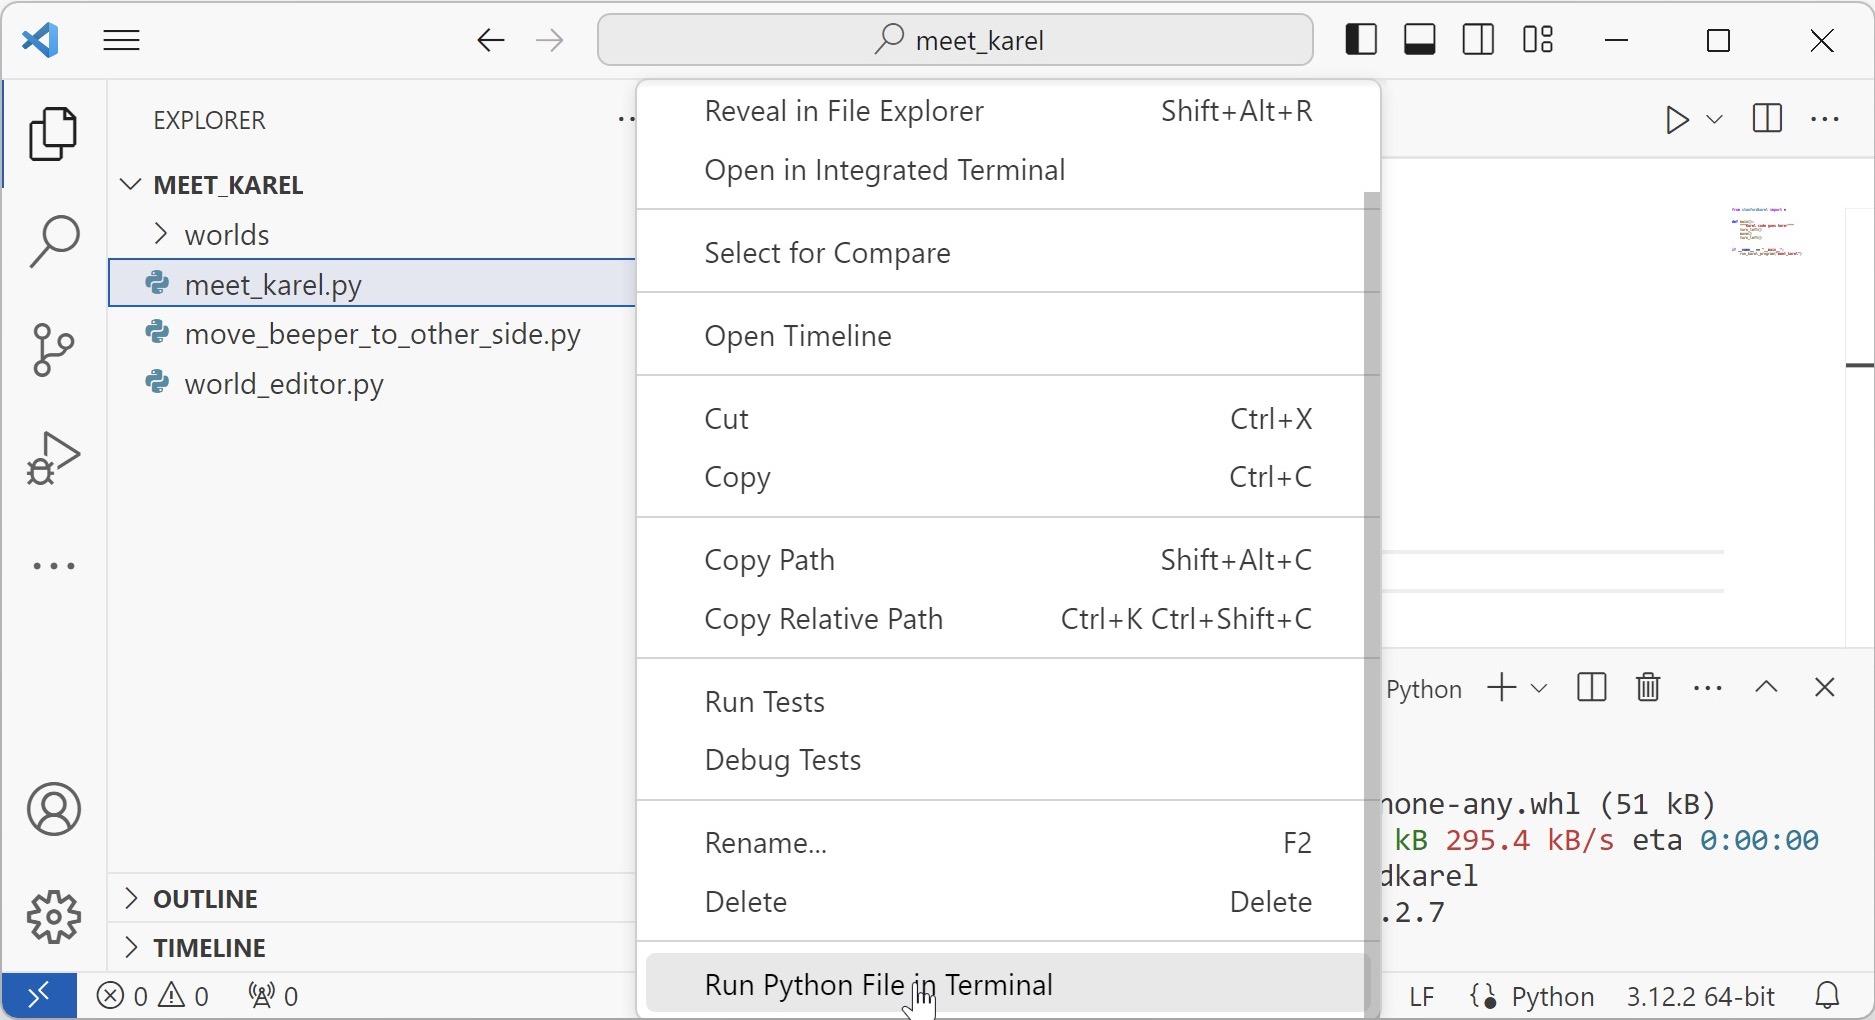
\includegraphics[width=.98\textwidth, trim={2.4mm 2mm 2mm 2mm},clip]{images/vscode_install/v9.jpg}};
    \drawshadow{image}
\end{tikzpicture}
\caption{} 
\label{fig:runmtkrl2}
\end{figure}

\begin{figure}[tbh!]
\begin{tikzpicture}
    \node[anchor=south west,inner sep=0] (image) at (0,0)
        {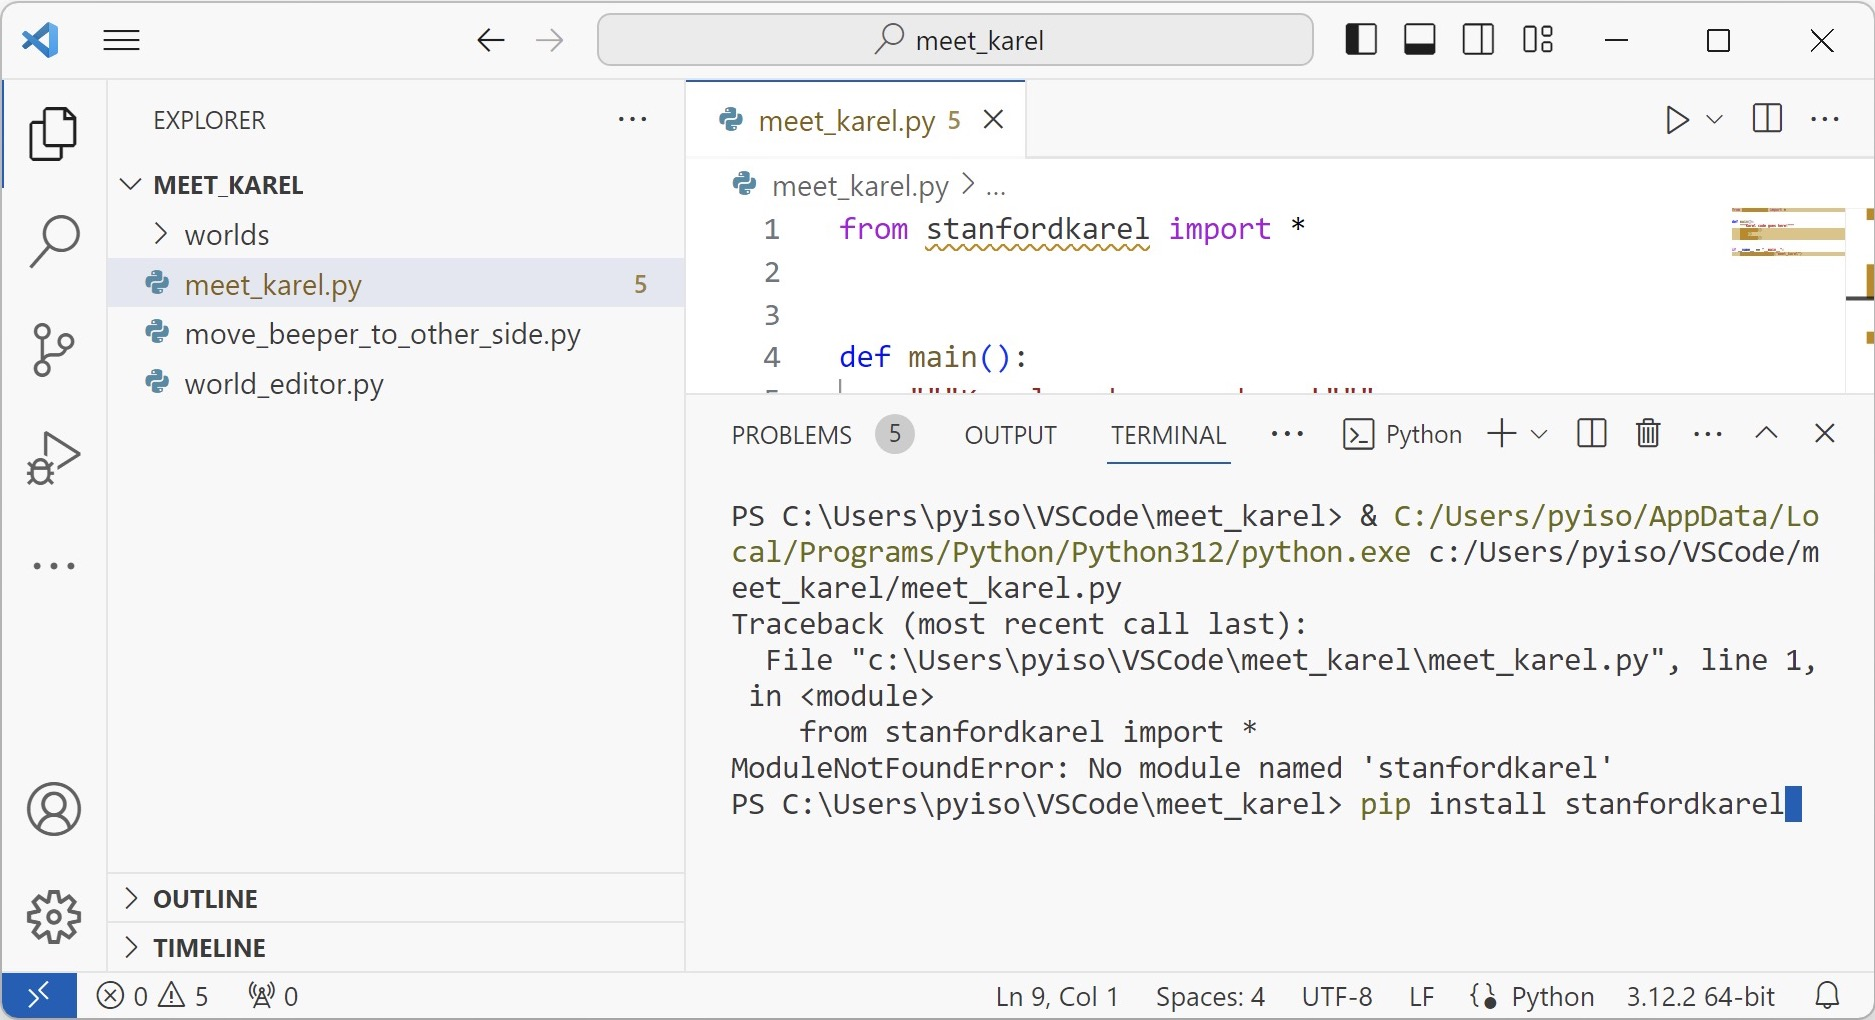
\includegraphics[width=.98\textwidth, trim={2.4mm 2mm 2mm 2mm},clip]{images/vscode_install/v8.jpg}};
    \drawshadow{image}
\end{tikzpicture}
\caption{} 
\label{fig:mtkrlfstrun}
\end{figure}
ခုနကပွင့်လာတဲ့ \fEnSnd{Terminal} မှာပဲ အောက်ပါကွန်မန်းကို \fEn{run} ပြီး \fEnSnd{stanfordkarel} လိုက်ဘရီကို အင်စတောလ်လုပ်ပါ။ 
%
\begin{minted}[frame=lines, framerule=0pt]{text}
pip install stanfordkarel
\end{minted}
%
ပုံ (\fRefNo{\ref{fig:mtkrlfstrun}}) မှာ အနီဝိုင်းထားတာကို ကြည့်ပါ။ အဲဒီအတိုင်းရိုက်ထည့်ပြီး \fEnSnd{Enter} ကီးနှိပ်ပါ။ ခဏကြာတဲ့အခါ အခုလို \fOpn{မက်ဆေ့ချ်}တွေ ကျလာပါလိမ့်မယ်။ 

%
\begin{minted}[frame=lines, framerule=0pt,escapeinside=ßß]{text}
ModuleNotFoundError: No module named 'stanfordkarel'
PS C:\Users\pyiso\VSCode\meet_karel> pip install stanfordkarel
Collecting stanfordkarel
  Downloading stanfordkarel-0.2.7-py3-none-any.whl (51 kB)
     ━━━━━━━━━━━━━━━━━━━━━━━ 51.9/51.9 kB 295.4 kB/s eta 0:00:00
Installing collected packages: stanfordkarel
ß\mytcboxinl[yellow]{Successfully installed stanfordkarel-0.2.7}ß
PS C:\Users\pyiso\VSCode\meet_karel> 
\end{minted}
%
ဟိုက်လိုက်ပြထားတဲ့ \fOpn{မက်ဆေ့ချ်} တွေ့ရရင် အင်စတောလ် အောင်မြင်လို့ပါ။ ပုံ (\fRefNo{\ref{fig:edtmtkrl}}) အယ်ဒီတာမှာလို သတိပေး လှိုင်းတွန့်မျဉ်းတွေ မရှိသင့်တော့ဘူး။ \fEnSnd{stanfordkarel} လိုက်ဘရီ အင်စတောလ် လုပ်ပြီးပြီမိုလို့ သတိပေးတာတွေ ပျောက်သွားသင့်တယ်။


\mytcboxinl{\fEnSnd{meet\_karel.py}} ဖိုင်ကို ညာကလစ်နှိပ်ပြီး \mytcboxinl{\fEnSnd{Run Python File in Terminal}} ပြန်လုပ်ကြည့်ပါ။ ပုံ (\fRefNo{\ref{fig:mtkrlprgm}}) မှာပြထားတဲ့ ကားရဲလ်ပရိုဂရမ် ပွင့်လာသင့်ပါတယ်။ \mytcboxinl{\fEnSnd{Run Program}} နှိပ်ကြည့်ပါ။ စက်ရုပ်လေး ကားရဲလ် နေရာရွေ့သွားတာ တွေ့ရမယ်။ \mytcboxinl{\fEnSnd{meet\_karel.py}} ကို အောက်ပါအတိုင်း ဖြည့်စွက်ရေးပါ။
\begin{figure}[tbh!]
\begin{tikzpicture}
    \node[anchor=south west,inner sep=0] (image) at (0,0)
        {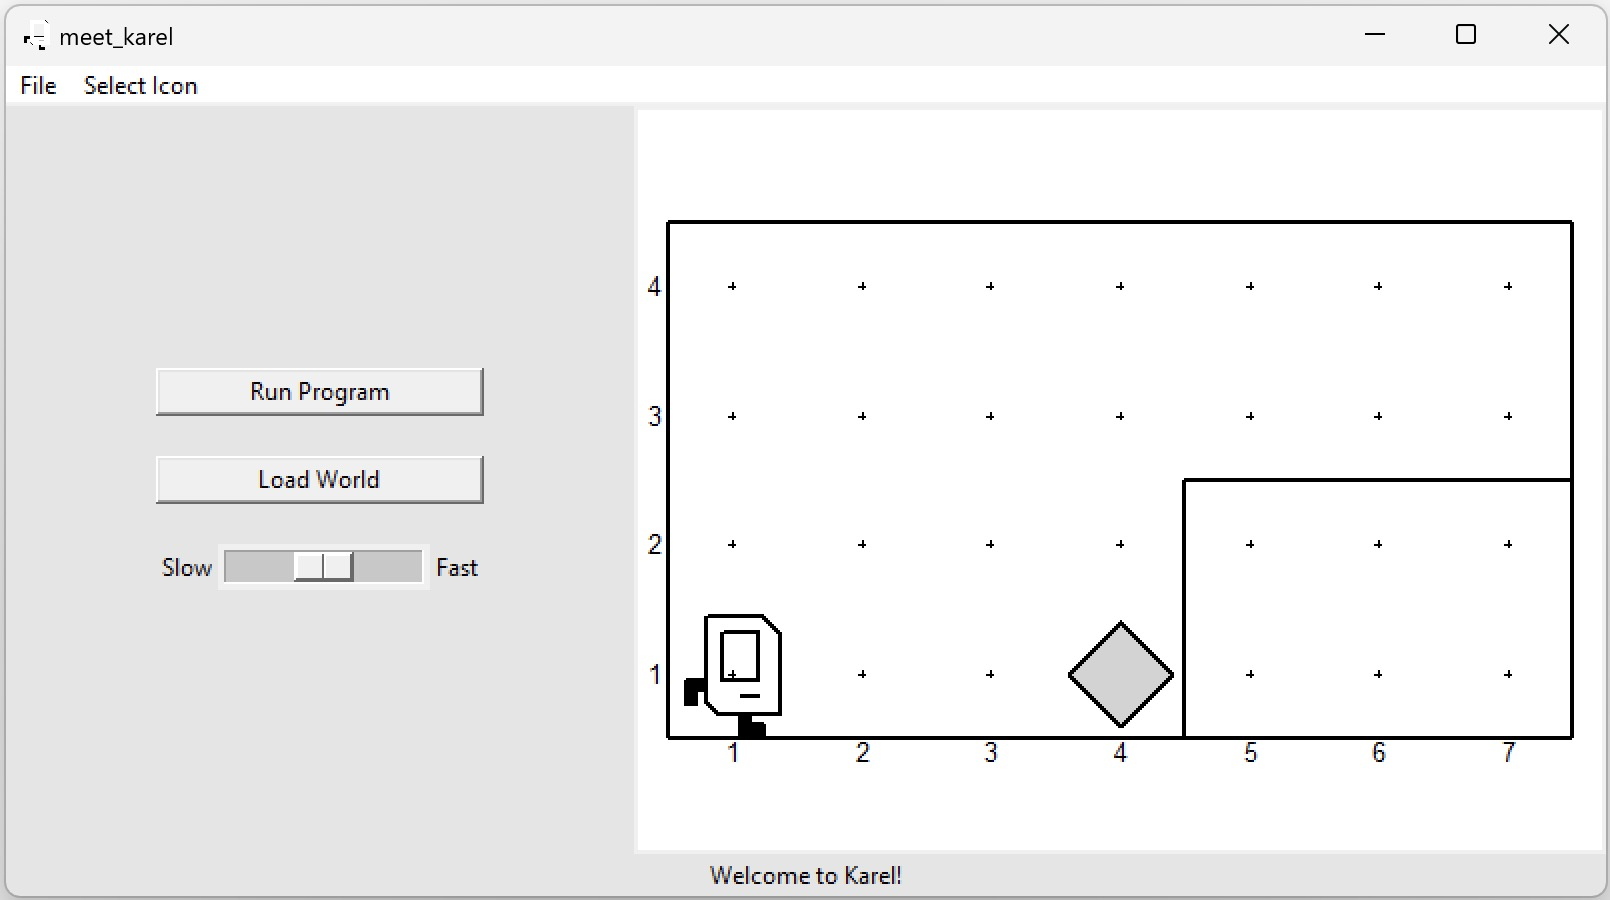
\includegraphics[width=.98\textwidth, trim={2.4mm 2mm 2mm 2mm},clip]{images/vscode_install/mtkrlprgm.jpg}};
    \drawshadow{image}
\end{tikzpicture}
\caption{} 
\label{fig:mtkrlprgm}
\end{figure}


%
\setlength{\fboxsep}{0pt}
\begin{minted}[frame=\mintframe, framerule=\mintrule,framesep= \mintsep, xleftmargin=\xlftmargin
                , bgcolor=mintbgcolor,rulecolor=mintrulecolor
                , python3=true]{python}
from stanfordkarel import *


def main():
    """Karel code goes here!"""
    move()
    move()
    move()
    pick_beeper()
    turn_left()
    move()
    move()

    turn_left()
    turn_left()
    turn_left()

    move()
    put_beeper()


if __name__ == "__main__":
    run_karel_program("meet_karel")
\end{minted}
%

\mytcboxinl{\fEnSnd{meet\_karel.py}} ဖိုင်ကို ညာကလစ်နှိပ်ပြီး \mytcboxinl{\fEnSnd{Run Python File in Terminal}} ပြန်လုပ်ကြည့်ပါ။ ကားရဲလ်ပရိုဂရမ် ပွင့်လာရင် \mytcboxinl{\fEnSnd{Run Program}} နှိပ်ကြည့်ပါ။ ဘိပါလေးကို နေရာရွှေ့ပေးပါလိမ့်မယ်။ အကယ်၍ ကားရဲလ်ပရိုဂရမ် မတက်လာရင် ကုဒ်ရေးတာမှားနေလို့ ဖြစ်နိုင်တယ်။ အပေါ်ကုဒ်နဲ့ နှိုင်းယှဉ်ပြီး ကြည့်ပါ။ \fEn{VS Code} အယ်ဒီတာမှာ အနီလှိုင့်တွန့်လေးတွေ ပြတဲ့နေရင် အဲဒီနေရာတွေမှာ ဆင်းတက်စ်မှားနေတာ ဖြစ်နိုင်တယ်။
%
\begin{mytcbox}
\fEn{VS Code} အယ်ဒီတာမှာ ပရိုဂရမ်ကုဒ်ပြင်ပြီး ပြန် \fEn{run} တဲ့အခါ ပထမ \fEn{run} ထားတဲ့ ပရိုဂရမ်ကို အရင်ပိတ်ဖို့လိုပါတယ်။ ဆိုလိုတာက \fEnSnd{meet\_karel.py} ကို \fEn{run} ထားတယ်ဆိုပါစို့။ ပုံ (\fRefNo{\ref{fig:mtkrlprgm}}) က ဝင်းဒိုးပွင့်လာမယ်။ \fEnSnd{meet\_karel.py} ကုဒ်ကို ပြင်ပြီး ပြန် \fEn{run} ချင်ရင် အဲဒီ ဝင်းဒိုးကို အရင်ပိတ်ရမယ်။ မဟုတ်ရင် ပြင်ထားတဲ့ ပရိုဂရမ်က ချက်ချင်း ပွင့်မလာဘူး။ ပထမ ဟာကို ပိတ်တော့မှပဲ နောက် \fEn{run} တဲ့ဟာ ပွင့်လာမှာ။ 
\end{mytcbox}
%
ဝိုက်ကွင်းကျန်နေတာက အဖြစ်များတဲ့ အမှားပါ။ ကျန်ခဲ့လို မရပါဘူး။ အင်ဒန့်တေးရှင်း \fEn{(indentation)} လုပ်ရမဲ့နေရာမှာ မလုပ်ထားရင်လည်း ပြဿနာဖြစ်တယ်။ \fCode{move}\fEn{,} \fCode{turn\_left} တွေကို ဘေးမျဉ်းညာဘက်ခွာပြီး အင်ဒန့်လုပ်ပေးရမယ်။ အဲဒါတွေ ဂရုမစိုက်မိရင် ဆင်းတက်စ်အမှားဖြစ်ပြီး ပရိုဂရမ် \fEn{run} လို့ မရနိုင်ဘူး။

\fEnSnd{Terminal} မှာ ထုတ်ပေးတဲ့ \fOpn{မက်ဆေ့ချ်}တွေကို ကြည့်ပြီးတော့လည်း ဘာပြဿနာဖြစ်နေလဲ မှန်းဆလို့ရနိုင်တယ်။ ဘာကြောင့်ဖြစ်နိုင်လဲ ဆက်စပ်စဉ်းစားလို့ ရတယ်။ ဥပမာ ဖြစ်တဲ့ပြဿနာအလိုက် အခုလိုတွေ့ရပါမယ်။ 
%
\begin{minted}[frame=lines, framerule=0pt,escapeinside=ßß]{text}
File "c:\Users\pyiso\VS Code\meet_karel\meet_karel.py", ß\mytcboxinl[yellow]{line 6}ß
    move(
          ^
    ß\mytcboxinl[yellow]{SyntaxError: '(' was never closed}ß
\end{minted}
%
%
\begin{minted}[frame=lines, framerule=0pt,escapeinside=ßß]{text}
File "c:\Users\pyiso\VS Code\meet_karel\meet_karel.py", ß\mytcboxinl[yellow]{line 7}ß
    move()
    ß\mytcboxinl[yellow]{IndentationError: unexpected indent}ß 
\end{minted}
%
%
\begin{minted}[frame=lines, framerule=0pt, escapeinside=ßß]{text}
Traceback (most recent call last):
  File "c:\Users\pyiso\VS Code\meet_karel\meet_karel.py", ß\mytcboxinl[yellow]{line 1}ß, 
        in <module>
    from stanfordkarel import *
    ß\mytcboxinl[yellow]{ModuleNotFoundError: No module named 'stanfordkarel'}ß
\end{minted}
%



\clearpage


\subsection*{VS Code တွင် Python ဖိုင် အသစ်ယူခြင်း}
\fEnSnd{MEET\_KAREL} ပင်မ ပရောဂျက်ဖိုဒါပေါ်မှာ ကလစ်နှိပ်ပါ။ ပုံမှာ ပြထားတဲ့ \mytcboxinl{\fEnSnd{New File}} အိုင်ကွန်ကိုနှိပ်ပါ။ ဖိုင်နံမည်ဖြည့်တဲ့ ဘောက်စ်လေး ပေါ်လာမယ်။ \fEn{Python} ဖိုင်တွေက \fEnSnd{.py} အိပ်စ်တန်းရှင်းနဲ့ ဖြစ်ရပါမယ်။ ဒါကြောင့် နံမည် ဖြည့်တဲ့အခါ \fEnSnd{.py} နဲ့ အဆုံးသတ်ပေးရပါမယ် (ဥပမာ \fEnSnd{hello.py})။ ကားရဲလ်ပရိုဂရမ်တစ်ခုကို \fEn{Python} ဖိုင်တစ်ခု ထားပါမယ်။ ပင်မ ပရောဂျက်ဖိုဒါ အောက်မှာပဲ တိုက်ရိုက်ရှိရပါမယ်။ 

နောက်ပိုင်း အဆင့်မြင့်လာရင် ပရိုဂရမ်တစ်ခုအတွက် ပရောဂျက်တစ်ခု ထားနိုင်တယ်။ ကုဒ်ဖိုင်တွေအပြင် ပရိုဂရမ်အတွက် လိုအပ်တဲ့ ရုပ်ပုံတွေ၊ အခြားဖိုင်တွေ (\fEn{config} ဖိုင်၊ \fEn{setting} ဖိုင် စသည်ဖြင့်) လည်း ပါနိုင်တယ်။ ပင်မပရောဂျက် အောက်မှာပဲ  ဖိုင်တွေက တိုက်ရိုက်ရှိဖို့လည်း မလိုတော့ဘူး။  ဆက်{\allowbreak}စပ်ရာ ဖိုင်တွေကို အမျိုးအစားအလိုက်၊  ဖန်ရှင်အလိုက် ဖိုဒါတွေခွဲပြီး  စနစ်ကျ စီစဉ်ဖွဲ့စည်း ထားရမှာပါ။ ပရောဂျက်တစ်ခုမှာ ဖိုင်တွေကို စနစ်တကျ စုဖွဲ့ထားဖို့ အရေးကြီးပါတယ်။

\begin{figure}[tbh!]
\begin{tikzpicture}
    \node[anchor=south west,inner sep=0] (image) at (0,0)
        {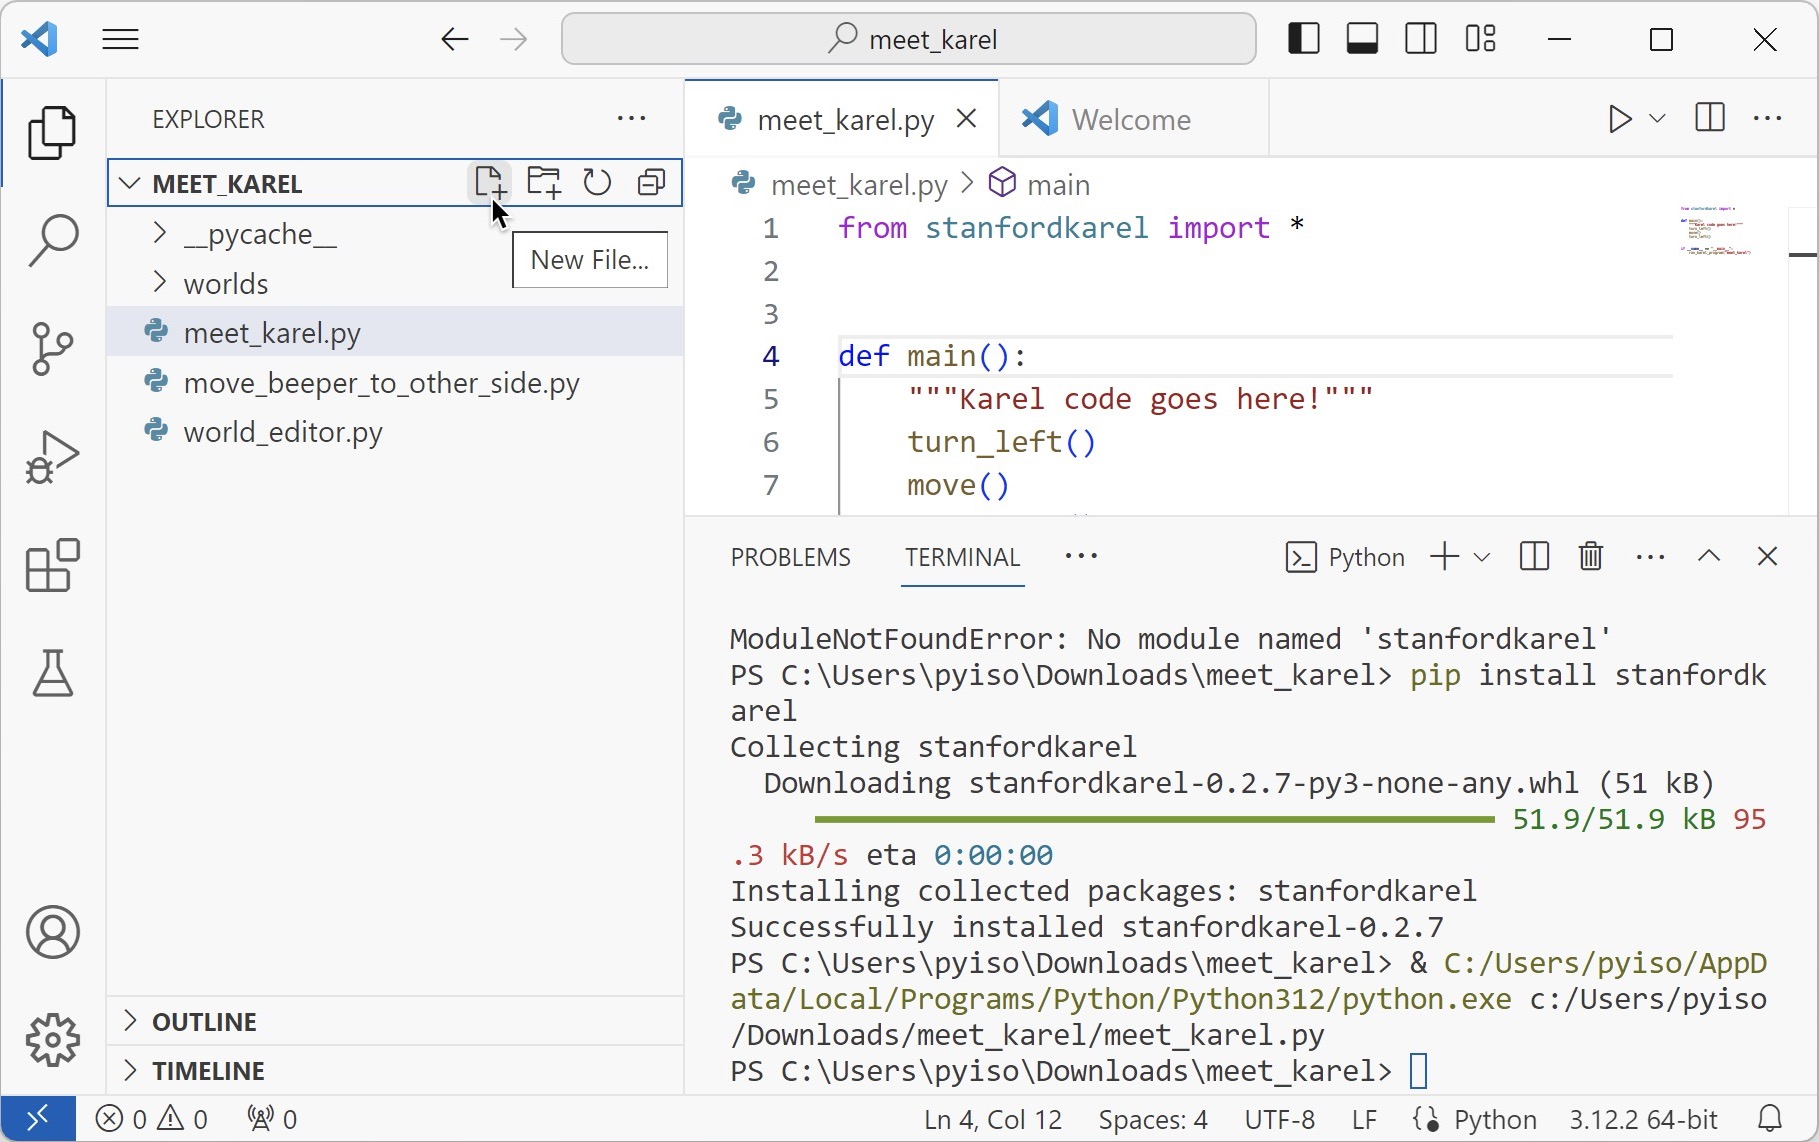
\includegraphics[width=.98\textwidth, trim={2.4mm 2mm 2mm 2mm},clip]{images/vscode_install/newfile.jpg}};
    \drawshadow{image}
\end{tikzpicture}
\caption{} 
\label{fig:vsnewfile}
\end{figure}

\clearpage








\afterpage{\blankpage}
